\documentclass[12pt,a4paper,twoside,ngerman,parskip=half*,bibtotoc]{scrbook}

\clubpenalty=10000
\widowpenalty=10000
\displaywidowpenalty=10000

\usepackage[ngerman]{babel}
\usepackage[T1]{fontenc}
\usepackage[utf8]{inputenc}

\usepackage{amsmath,amssymb,amsthm,mathtools,graphicx}

\usepackage{tikz}
\usetikzlibrary{arrows, automata, calc, matrix, positioning}

\usepackage{cite, xcolor}
\definecolor{lgray}{gray}{0.7}
\definecolor{commentShadeColor}{rgb}{1.0,.9,.6}
\definecolor{commentTextColor}{rgb}{.2,.2,.2}
\definecolor{CommentFrameColor}{rgb}{.3,.3,.3}%

\usepackage{paralist}

\usepackage{lmodern}

\usepackage{ifthen}

\addtokomafont{sectioning}{\rmfamily\boldmath}

\newtheoremstyle{mythmstyle}% name of the style to be used
  {5pt}% measure of space to leave above the theorem. E.g.: 3pt
  {4pt}% measure of space to leave below the theorem. E.g.: 3pt
  {\itshape}% name of font to use in the body of the theorem
  {}% measure of space to indent
  {\bfseries}% name of head font
  {.}% punctuation between head and body
  {0.5em}% space after theorem head; " " = normal interword space
{\textbf{\thmname{#1}\thmnumber{ #2}\thmnote{ (\textit{#3})}}}% Manually specify head
\theoremstyle{mythmstyle}
\newtheorem{Def}{Definition}[chapter]
\newtheorem{Satz}[Def]{Satz}
\newtheorem{Bsp}[Def]{Beispiel}
\newtheorem{Lem}[Def]{Lemma}
\newtheorem{Kor}[Def]{Korollar}
\newtheorem{Prop}[Def]{Proposition}
\newtheorem{Bem}[Def]{Bemerkung}

\newcommand{\oBdA}{oBdA}
\newcommand{\OBdA}{OBdA}
\newcommand{\EIO}{EIO}
\newcommand{\MIA}{MIA}
\newcommand{\MEIO}{\mbox{MEIO}}

\newcommand{\may}[1][\empty]{%
  \ifthenelse{\equal{#1}{\empty}}{\ensuremath{\dashrightarrow}}
  {\ensuremath{\overset{#1}{\dashrightarrow}}
  }}

\newcommand{\must}[1][\empty]{%
  \ifthenelse{\equal{#1}{\empty}}{\ensuremath{\longrightarrow}}
  {\ensuremath{\overset{#1}{\longrightarrow}}
  }}

\newcommand{\nmay}[1][\empty]{%
  \hspace{0.2cm}\not\hspace{-0.2cm}\may[#1]
  }

\newcommand{\nmust}[1][\empty]{%
  \hspace{0.2cm}\not\hspace{-0.2cm}\must[#1]
  }

\newcommand{\anmust}[1][\empty]{%
  \hspace{0.25cm}\not\hspace{-0.25cm}\must[#1]
  }

\newcommand{\weakmay}[1][\empty]{%
  \ifthenelse{\equal{#1}{\empty}}{\ensuremath{=\Rightarrow}}
  {\ensuremath{\overset{#1}{=\Rightarrow}}
  }}

\newcommand{\weakmust}[1][\empty]{%
  \ifthenelse{\equal{#1}{\empty}}{\ensuremath{\Longrightarrow}}
  {\ensuremath{\overset{#1}{\Longrightarrow}}
  }}

\newcommand{\nweakmust}[1][\empty]{%
  \ensuremath{\hspace{0.2cm}\not\hspace{-0.2cm}\weakmust[#1]}
  }

\newcommand{\nweakmay}[1][\empty]{%
  \ensuremath{\hspace{0.25cm}\not\hspace{-0.25cm}\weakmay[#1]}
  }


\newcommand{\lweakmay}[1][\empty]{%
  \ifthenelse{\equal{#1}{\empty}}{\ensuremath{==\Rightarrow}}
  {\ensuremath{\overset{#1}{==\Rightarrow}}
  }}

\DeclareRobustCommand{\maRel}{\ensuremath{%\text{\reflectbox{\rotatebox[origin=c]{180}{$
  \sqsubseteq%$}}}
  }}

\newcommand{\prune}{\ensuremath{\mathrm{prune}}}
\newcommand{\cont}{\ensuremath{\mathrm{cont}}}
\newcommand{\Sig}{\ensuremath{\mathrm{Sig}}}
\newcommand{\Synch}{\ensuremath{\mathrm{Synch}}}
\newcommand{\NF}{\ensuremath{NF}}
\newcommand{\asimp}{\ensuremath{\mathrm{as}\text{-}\mathrm{impl}}}
\newcommand{\wasimp}{\ensuremath{\mathrm{w}\text{-}\mathrm{as}\text{-}\mathrm{impl}}}

\newcommand{\EBbaRel}{\ensuremath{\sqsubseteq _E^\mathrm{B}}}
\newcommand{\ECbaRel}{\ensuremath{\sqsubseteq _E^\mathrm{C}}}
\newcommand{\EbaRel}{\ensuremath{\sqsubseteq _E}}
\newcommand{\EBRel}{\ensuremath{\maRel _E^\mathrm{B}}}
\newcommand{\ECRel}{\ensuremath{\maRel _E^\mathrm{C}}}
\newcommand{\ERel}{\ensuremath{\maRel _E}}
\newcommand{\EsatAs}{\ensuremath{\hspace{0.05cm}sat_\mathrm{as}^E\hspace{0.05cm}}}
\newcommand{\StET}{\ensuremath{StET}}
\newcommand{\PrET}{\ensuremath{PrET}}
\newcommand{\MIT}{\ensuremath{MIT}}
\newcommand{\ET}{\ensuremath{ET}}
\newcommand{\EL}{\ensuremath{EL}}

\newcommand{\QBbaRel}{\ensuremath{\sqsubseteq _{Qui}^\mathrm{B}}}
\newcommand{\QCbaRel}{\ensuremath{\sqsubseteq _{Qui}^\mathrm{C}}}
\newcommand{\QbaRel}{\ensuremath{\sqsubseteq _{Qui}}}
\newcommand{\QBRel}{\ensuremath{\maRel _{Qui}^\mathrm{B}}}
\newcommand{\QCRel}{\ensuremath{\maRel _{Qui}^\mathrm{C}}}
\newcommand{\QRel}{\ensuremath{\maRel _{Qui}}}
\newcommand{\QsatAs}{\ensuremath{\hspace{0.05cm}sat_\mathrm{as}^{Qui}\hspace{0.05cm}}}
\newcommand{\StQT}{\ensuremath{StQT}}
\newcommand{\QET}{\ensuremath{QET}}

\newcommand{\DBbaRel}{\ensuremath{\sqsubseteq _{Div}^\mathrm{B}}}
\newcommand{\DCbaRel}{\ensuremath{\sqsubseteq _{Div}^\mathrm{C}}}
\newcommand{\DbaRel}{\ensuremath{\sqsubseteq _{Div}}}
\newcommand{\DBRel}{\ensuremath{\maRel _{Div}^\mathrm{B}}}
\newcommand{\DCRel}{\ensuremath{\maRel _{Div}^\mathrm{C}}}
\newcommand{\DRel}{\ensuremath{\maRel _{Div}}}
\newcommand{\DsatAs}{\ensuremath{\hspace{0.05cm}sat_\mathrm{as}^{Div}\hspace{0.05cm}}}
% \newcommand{\DBaRel}{\ensuremath{\sqsubseteq _{Div_{\mathrm{alt}}}^\mathrm{B}}}
% \newcommand{\DCaRel}{\ensuremath{\sqsubseteq _{Div_{\mathrm{alt}}}^\mathrm{C}}}
% \newcommand{\DaRel}{\ensuremath{\sqsubseteq _{Div_{\mathrm{alt}}}}}
\newcommand{\asRel}{\ensuremath{\sqsubseteq _{\mathrm{as}}}}
\newcommand{\wasRel}{\ensuremath{\sqsubseteq _{\mathrm{w}\text{-}\mathrm{as}}}}
\newcommand{\StDT}{\ensuremath{StDT}}
\newcommand{\PrDT}{\ensuremath{PrDT}}
\newcommand{\EDT}{\ensuremath{EDT}}
\newcommand{\EDL}{\ensuremath{EDL}}
\newcommand{\QDT}{\ensuremath{QDT}}
\newcommand{\DT}{\ensuremath{DT}}

%%%%%%%%%%%%%%%%%%%%%%%%%%%%%%%%%%%%%%%%%%%%%%%%%%%%%%%%%%%%%%%%%%%%%%%%%%%%%%
% \newcommand{\comments}{true} % auskommentieren um Kommentare zu entfernen
%%%%%%%%%%%%%%%%%%%%%%%%%%%%%%%%%%%%%%%%%%%%%%%%%%%%%%%%%%%%%%%%%%%%%%%%%%%%%%

\ifthenelse{\isundefined{\comments}}
{% keine Kommentare
  \newcommand{\TODO}[1]{}
}
{% Kommentare werden hervorhoben
 \newcommand{\TODO}[1]{%
      \fcolorbox{CommentFrameColor}{commentShadeColor}{%
      \scriptsize T\!O\!D\!O: #1
  }}
}

\begin{document}

\KOMAoptions{twoside = false}

% \frontmatter

% \begin{titlepage}
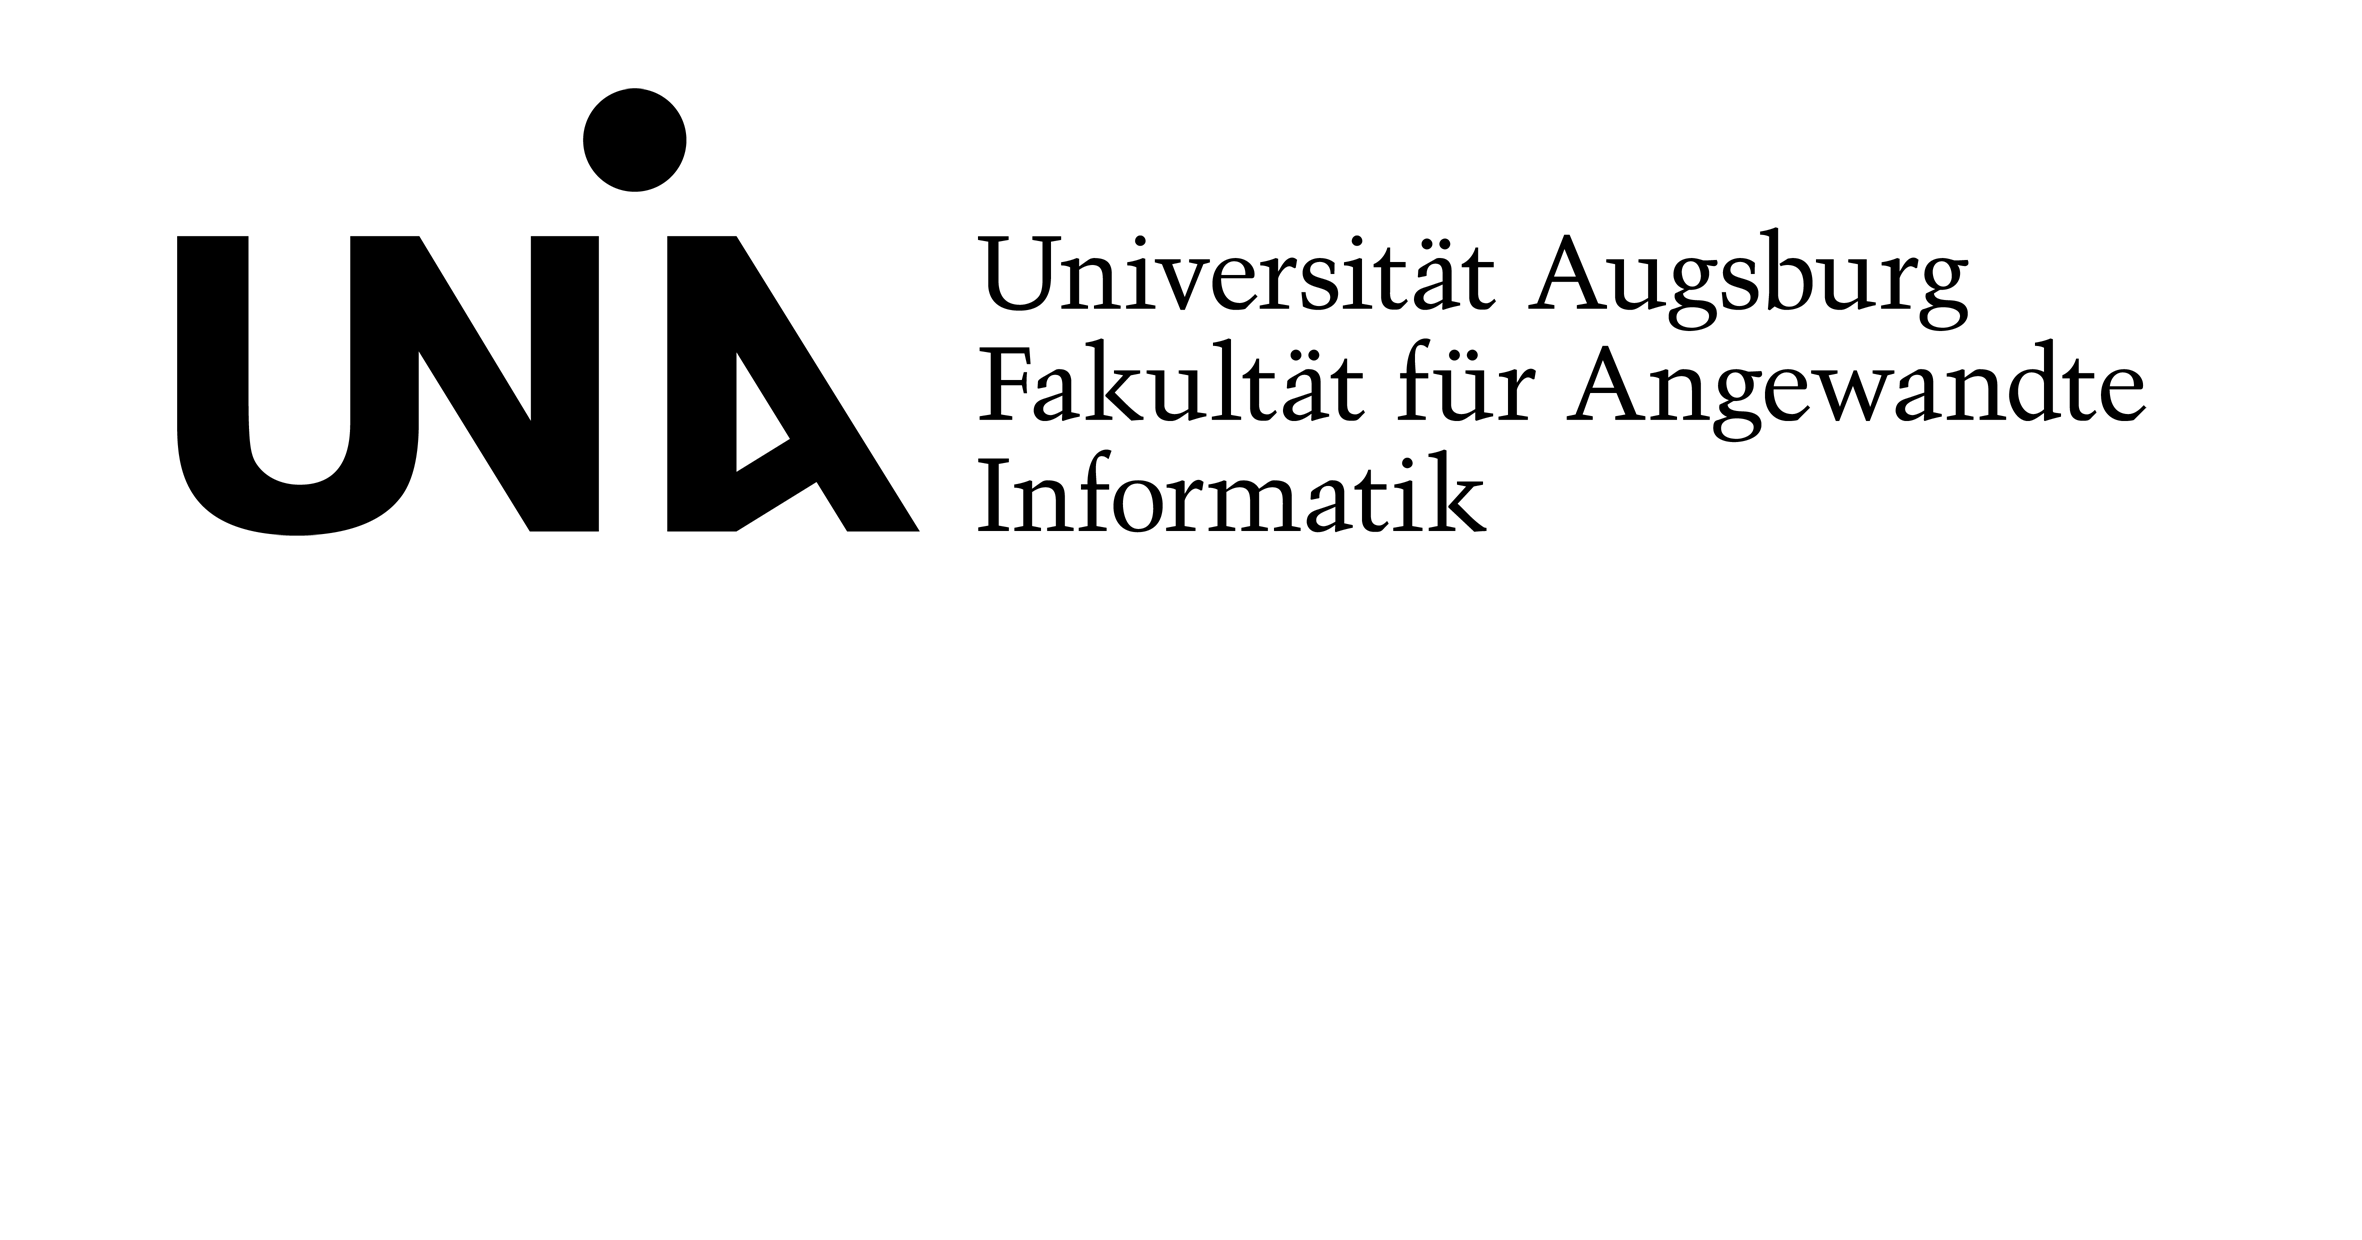
\includegraphics[width=0.4\textwidth]{Uni_Aug_Logo_FAI_schwarz.png}
\vspace{-1cm}
\begin{center}
  \LARGE \textsc{Masterarbeit}\\
  \normalsize im Studiengang Master Informatik\\
  \vfill
  \Huge \textsc{Stillstand,Divergenz und modale Spezifikation}\\
  \vfill
  \Large Universität Augsburg\\
  Fakultät für Angewandte Informatik\\
  Theorie verteilter Systeme\\
  \vspace{2cm}
  \rmfamily \large \textbf{Aufgabensteller:} Prof.\;Dr.\;Walter Vogler
\end{center}
\vspace{1.5cm}
\large \textbf{%eingereicht 
  von:}
Ayleen Schinko\\
\textbf{%eingereicht am:}
  Stand:}
\today\\
  \TODO{überarbeiten}
\end{titlepage}


% \KOMAoptions{twoside}

% \clearpage
% \thispagestyle{empty}

% \tableofcontents{}

\mainmatter{}

% \chapter{Einleitung}
{\large\textbf{Stand: \today{}}}

\textbf{TODO}

\TODO{schreiben}

\TODO{Quellen und Literarturverweise}


% \clearpage
% \thispagestyle{empty}

\chapter{Grundlagen}

\chapter{Definitionen}
{\large\textbf{Stand: \today{}}}\\

Kombination aus~\cite{Vogler2015FailSem} und~\cite{Schinko2016BA} mit
Einflüssen von~\cite{Vogler2016MIA3}:

\begin{Def}[Modal Error-I/O-Transitionssystem]
  Ein \emph{Modal Error-I/O-Transitionssystem (\MEIO{})} ist ein Tupel
  $(P,I,O,\must,\may,p_0,E)$ mit:
  \begin{itemize}
    \item $P$: Menge der \emph{Zustände},
    \item $p_0\in P$: \emph{Startzustand},
    \item $I,O$: disjunkte Mengen der (sichtbaren) \emph{Input-} und
      \emph{Output-Aktionen},
    \item $\must{} \subseteq P\times \Sigma_{\tau}\times P$:
      \emph{must-Transitions-Relation},
    \item $\may{} \subseteq P\times \Sigma_{\tau}\times P$:
      \emph{may-Transitions-Relation},
    \item $E\subseteq P$: Menge der \emph{Fehler-Zustände}.
  \end{itemize}
  Es wird vorausgesetzt, dass $\must\subseteq\may$ (\emph{syntaktische
  Konsistenz}) gilt.\\
  Das \emph{Alphabet} bzw.\ die Aktionsmenge eines \MEIO{} ist $\Sigma = I\cup
  O$. Die \emph{interne Aktion} $\tau$ ist nicht in $\Sigma$ enthalten. Jedoch
  gilt $\Sigma_{\tau} := \Sigma \cup \{\tau\}$. Die \emph{Signatur} eines
  \MEIO{}s entspricht $\Sig (P)=(I,O)$.\\
  Falls $\must =\may$ gilt, wird $P$ auch \emph{Implementierung} genannt.
\end{Def}

Implementierungen entsprechen den in~\cite{Schinko2016BA} behandelten
\EIO{}s.\\
Must-Transitionen sind Transitionen, die von einer Verfeinerung implementiert
werden müssen. Die may-Transitionen sind hingegen die zulässigen Transitionen
für eine Verfeinerung.\\
\MEIO{}s  werden in dieser Arbeit durch ihre Zustandsmenge (z.B.\ $P$)
identifiziert und falls notwendig werden damit auch die Komponenten indiziert
(z.B.\ $I_P$ anstatt $I$). Falls der \MEIO{} selbst bereits einen Index hat
(z.B.\ $P_1$) kann an der Komponente die Zustandsmenge als Index wegfallen und
nur noch der Index des gesamten Automaten verwendet werden (z.B.\ $I_1$ anstatt
$I_{P_1}$). Zusätzlich stehen $i,o,a,\omega$ und $\alpha$ für Buchstaben aus
den Alphabeten $I,O,\Sigma ,O\cup\{\tau\}$ und $\Sigma_\tau$.\\
Es wir die Notation $p\may[\alpha] p'$ für $(p,\alpha,p')\in\may$ und
$p\may[\alpha]$ für $\exists p':(p,\alpha,p')\in\may$ verwendet. Dies kann
entsprechend auf Buchstaben-Sequenzen $w\in\Sigma_{\tau}^*$ erweitert werden zu
$p\may[w]p'$ ($p\may[w]$) steht für die Existenz eines Laufes $p\may[\alpha _1]
p_1\may[\alpha _2]\dots p_{n-1}\may[\alpha _n] p'$ ($p\may[\alpha _1]
p_1\may[\alpha _2]\dots p_{n-1}\may[\alpha _n]$) mit $w=\alpha _1\dots \alpha
_n$.\\
Desweiteren soll $w|_B$ die Aktions-Sequenz bezeichnen, die man erhält, wenn
man aus $w$ alle Aktionen löscht, die nicht in $B\subseteq\Sigma$ enthalten
sind. $\widehat{w}$ steht für $w|_{\Sigma}$. Es wir $p\weakmay[w] p'$
für ein $w\in\Sigma ^*$ geschrieben, falls $\exists
w'\in\Sigma_{\tau}^*:\widehat{w'}=w\land p\may[w']p'$, und $p\weakmay[w]$,
falls $p\weakmay[w] p'$ für ein beliebiges $p'$ gilt. Falls $p_0\weakmay[w] p$
gilt, dann wird $w$ \emph{Trace} genannt und $p$ ist ein \emph{erreichbarer
Zustand}.\\
Analog zu $\may$ und $\weakmay$ werden $\must$ und $\weakmust$ für die
entsprechenden Relationen der must-Transition verwendet.\\
Outputs und die interne Aktion werden \emph{lokale Aktionen} genannt, da sie
lokal vom ausführenden \MEIO{} kontrolliert sind. Um eine Erleichterung der
Notation zu erhalten, soll gelten, dass $p\nmust[a]$ und $p\nmay[a]$ für
$\nexists p': p\must[a]p'$ und $\nexists p': p\may[a]p'$ stehen soll. In
Graphiken wird eine Aktion $a$ als $a?$ notiert, falls $a\in I$ und $a!$, falls
$a\in O$. Must-Transitionen (may-Transitionen) werden als durchgezogener Pfeil
gezeichnet (gestrichelter Pfeil). Entsprechend der syntaktischen Konsistenz
repräsentiert jede gezeichnete must-Transition auch gleichzeitig die
zugrundeliegende may-Transitionen.

\begin{Def}[Parallelkomposition]
  \label{ParallelDef}
  Zwei \MEIO{}s $P_1 = (P_1,I_1,O_1,{\must_1,}{\may_1,}$ $p_{01},E_1)$ und $P_2 =
  (P_2,I_2,O_2,\must_2,\may_2,p_{02},E_2)$ sind \emph{komponierbar}, falls
  $O_1\cap O_2=\emptyset$. Für solche \MEIO{}s ist die
  \emph{Parallelkomposition} $P_{12} := P_1\|P_2=((P_1\times P_2), I, O,
  {\must_{12},}$ ${\may_{12},}$ $(p_{01}, p_{02}), E)$ definiert mit:
  \TODO{erzwungenen Zeilenumbrüche kontrollieren}
  \begin{itemize}
    \item $I=(I_1\cup I_2)\backslash (O_1\cup O_2)$,
    \item $O=(O_1\cup O_2)$,
  \item $\begin{aligned}[t]
      \must_{12} & = \left\{\left((p_1,p_2),\alpha,(p_1',p_2)\right) \mid p_1
      \must[\alpha]_1 p_1', \alpha\in\Sigma_{\tau}\backslash
      \Synch(P_1,P_2)\right\}\\
        &\cup \left\{\left((p_1,p_2),\alpha,(p_1,p_2')\right) \mid p_2
      \must[\alpha]_2 p_2', \alpha\in\Sigma_{\tau}\backslash
      \Synch(P_1,P_2)\right\}\\
        &\cup \left\{\left((p_1,p_2),\alpha,(p_1',p_2')\right) \mid p_1
      \must[\alpha]_1 p_1', p_2 \must[\alpha]_2 p_2', \alpha\in
      \Synch(P_1,P_2)\right\}
    \end{aligned}$
  \item $\begin{aligned}[t]
      \may_{12} & = \left\{\left((p_1,p_2),\alpha,(p_1',p_2)\right) \mid p_1
      \may[\alpha]_1 p_1', \alpha\in\Sigma_{\tau}\backslash
      \Synch(P_1,P_2)\right\}\\
        &\cup \left\{\left((p_1,p_2),\alpha,(p_1,p_2')\right) \mid p_2
      \may[\alpha]_2 p_2', \alpha\in\Sigma_{\tau}\backslash
      \Synch(P_1,P_2)\right\}\\
        &\cup \left\{\left((p_1,p_2),\alpha,(p_1',p_2')\right) \mid p_1
      \may[\alpha]_1 p_1', p_2 \may[\alpha]_2 p_2', \alpha\in
      \Synch(P_1,P_2)\right\}
    \end{aligned}$
  \item $\begin{aligned}[t]
      E & = (P_1\times E_2) \cup (E_1\times P_2) &&\text{geerbte
      Kommunikationsfehler}\\
        &\quad\left. \begin{aligned}
        &\cup \left\{(p_1,p_2) \mid \exists a \in O_1\cap I_2 : p_1
        \may[a]\land p_2\nmust[a]\right\}\\
        &\cup \left\{(p_1,p_2) \mid \exists a\in I_1\cap O_2 :
        p_1\nmust[a]\land p_2\may[a]\right\}
        \end{aligned}\hspace{0.3cm}\right\} &&\text{neue Kommunikationsfehler}
    \end{aligned}$
  \end{itemize}
  Dabei bezeichnet $\Synch(P_1,P_2)=(I_1\cap O_2)\cup (O_1\cap I_2)\cup
  (I_1\cap I_2)$ die Menge der zu \emph{synchronisierenden Aktionen}. Die
  synchronisierten Aktionen werden als Output bzw. Input der Komposition
  beibehalten.
\end{Def}

Ein neuer Kommunikationsfehler entsteht, wenn einer der \MEIO{}s die
Möglichkeit für einen Output hat (may-Transition) und der andere \MEIO{} der
passenden Input nicht erzwingt (keine must-Transition vorhanden). Es muss also
in möglichen Implementierungen nicht wirklich zu diesem Kommunikationsfehler
kommen, da die Output-Transition nicht zwingender maßen implementiert werden
muss.\\
Wie bereits in~\cite{Schinko2016BA} kann es durch die Synchronisation von
Inputs zu keinen neuen Kommunikationsfehler kommen, da dies in beiden Automaten
keine lokal kontrollierte Aktion ist. Falls jedoch nur einer der Automaten die
Möglichkeit für einen Input hat, der synchronisiert wird, besteht diese
Möglichkeit in der Parallelkomposition nicht mehr. Es kann also in der
Kommunikation mit einem weiteren \MEIO{} dort zu einen neuen
Kommunikationsfehler kommen.

\begin{Def}[Simulation]
  \label{SimDef}
  Eine \emph{(starke) alternierende Simulation} ist eine Relation $R\subseteq P
  \times Q$ auf zwei \MEIO{}s $P$ und $Q$, falls für alle $(p,q)\in R$ gilt:
  \begin{enumerate}
    \item $q\must[\alpha] q'$ impliziert $p\must[\alpha] p'$ für ein $q'$ mit
      $pRq'$,
    \item $p\may[\alpha] p'$ impliziert $q\may[\alpha] q'$ für ein $p'$ mit
      $pRq'$,
  \end{enumerate}
  Die Vereinigung \asRel{} aller dieser Relationen wird als \emph{(starke)
  as-Verfeinerung(-s Relation)} (auch modal Verfeinerung) bezeichnet. Es wird
  $P\asRel Q$ geschrieben, falls $p_0\asRel q_0$ gilt, und $P$
  \emph{as-verfeinert} $Q$ \emph{(stark)} oder $P$ ist eine \emph{(starke)
  as-Verfeinerung} von $Q$.\\
  Für einen \MEIO{} $Q$ und eine Implementierung mit $P$ mit $P\asRel{}Q$, ist
  $P$ eine \emph{as"=Implementierung} von $Q$ und es wird $\asimp (Q)$ für die
  Menge aller as"=Implementierungen von $Q$ verwendet.
\end{Def}

Die Parallelkomposition von Wörtern und Mengen kann aus~\cite{Schinko2016BA}
übernommen werden.

\begin{Def}[Parallelkomposition auf Traces]\mbox{}
  \begin{itemize}
    \item Für zwei Wörter $w_1\in\Sigma _1$ und $w_2\in\Sigma _2$ ist
      deren Parallelkomposition definiert als: $w_1\| w_2:=\left\{w\in
      (\Sigma _1\cup\Sigma _2)^*\mid w|_{\Sigma _1}=w_1\wedge w|_{\Sigma
    _2}=w_2\right\}$.
    \item Für zwei Mengen von Wörtern bzw. Sprachen $W_1\subseteq \Sigma
      ^*_1$ und $W_2\subseteq \Sigma ^*_2$ ist deren Parallelkomposition
      definiert als: $W_1\| W_2:=\bigcup\hspace{1pt}\left\{w_1\| w_2\mid
      w_1\in W_1\wedge w_2\in W_2\right\}$.
  \end{itemize}
\end{Def}

Ebenso können die Definitionen der Funktionen \prune{} und \cont{} zum
Abschneiden und Verlängern von Traces aus~\cite{Schinko2016BA} übernommen
werden.

\begin{Def}[Pruning- und Fortsetzungs-Funktion]\mbox{}
  \begin{itemize}
    \item $\prune{}:\Sigma ^*\rightarrow\Sigma ^*, w\mapsto u$, mit $w=uv,
      u=\varepsilon\footnotemark\vee u\in\Sigma ^*\cdot I$ und $v\in O^*$,
    \footnotetext{$\varepsilon$ bezeichnet das leere Wort}
    \item $\cont{}:\Sigma ^*\rightarrow\mathfrak{P}(\Sigma ^*)\footnotemark,
      w\mapsto\left\{wu\mid u\in\Sigma ^*\right\}$,
    \footnotetext{$\mathfrak{P}(M)$ bezeichnet die Potenzmenge der Menge $M$}
    \item $\cont{}:\mathfrak{P}(\Sigma ^*)\rightarrow\mathfrak{P}(\Sigma ^*),
      L\mapsto\bigcup\hspace{1pt}\left\{\cont{}(w)\mid w\in L\right\}$.
  \end{itemize}
\end{Def}

\begin{Def}[Sprache]
  \label{LDef}
  Die \emph{(maximale) Sprache} eines \MEIO{}s $P$ ist $L(P) := \left\{w\in
  \Sigma ^* \mid \exists P'\in\asimp (P) : p'_0\weakmust[w]
  \right\}$.\\
  Für zwei komponierbare \MEIO{}s $P_1$ und $P_2$ gilt: $L_{12} := L(P_{12}) =
  L_1\|L_2$.
\end{Def}


\section{Allgemeine Folgerungen}
\label{saetzeKapitel}

\begin{Prop}[Sprache und Implementierungen]
  \label{LImpProp}
  Für die Sprache eines \MEIO{}s $P$ gilt $L(P) \subseteq \underset{P'\in\asimp
  (P)}{\bigcup} L(P')$.
\end{Prop}
\begin{proof}\mbox{}\\
  Sei $P'$ die as-Implementierung von $P$, die alle may- und must-Transitionen
  von $P$ implementiert. Die Definition von $P'$ lautet also:
  \begin{itemize}
    \item $P'=P$,
    \item $p'_0=p_0$,
    \item $I_{P'}=I_P$ und $O_{P'}=O_P$,
    \item $\must _{P'} =\may _{P'} = \may _P$,
    \item $E_{P'}=\emptyset$.
  \end{itemize}
  Die entsprechende starke as"=Verfeinerungs"=Relation $\mathcal{R}$, die
  zwischen $P'$ und $P$ gilt, ist die Identitäts-Relation zwischen den
  Zuständen der Transitionssysteme. Für~\ref{SimDef}.3 betrachten wir $(p,p)
  \in\mathcal{R}$ mit $p\may[\alpha]_{P'} p'$ in $P'$. Diese Transition muss
  auch in $P$ existieren und da $\mathcal{R}$ die Identitäts-Relation ist auch
  $(p',p')\in\mathcal{R}$ gelten. Alle must"=Transitionen in $P$ haben zugrunde
  liegende may"=Transitionen. Es gibt also zu jeder must"=Transition $p
  \must[\alpha]_P p'$ in $P$ auch die Transition $p\must[\alpha]_{P'} p'$. Es
  folgt dann auch $(p',p') \in \mathcal{R}$ und dadurch ist auch~\ref{SimDef}.2
  erfüllt. Der erste Punkt von~\ref{SimDef} gilt, da $E_{P'}$ leer ist.\\
  Für alle $w\in L(P) = \left\{w\in \Sigma ^* \mid p_0\weakmay[w]_P\right\}$
  gilt $w\in L(P') = \left\{w\in \Sigma ^* \mid p'_0 \weakmust[w]_{P'}
  \right\}$, da alle Transitionen von $P$ in $P'$ implementiert werden.
\end{proof}

\begin{Prop}[Sprache der Parallelkomposition]
  \label{LParallelProp}
  Für zwei komponierbare \MEIO{}s $P_1$ und $P_2$ gilt: $L_{12} := L(P_{12}) =
  L_1\|L_2$.
\end{Prop}
\begin{proof}
  Jedes Wort, dass in $L_{12}$ enthalten ist, hat einen einen entsprechenden
  Ablauf, der in $P_{12}$ ausführbar ist. Dieser Ablauf kann auf Abläufe von
  $P_1$ und $P_2$ projiziert werden und die Projektionen sind dann in $L_1$ und
  $L_2$ enthalten.\\
  In einer Parallelkomposition werden die Wörter der beiden \MEIO{}s gemeinsam
  ausgeführt, falls es sich um synchronisierte Aktionen handelt, und
  verschränkt sequenziell, wenn es sich um unsynchronisierte Aktionen handelt.
  Somit sind alle Wörter aus $L_1\|L_2$ auch Wörter der Parallelkomposition
  $L(P_{12})$.
\end{proof}

\begin{Lem}[w-as-Verfeinerung und Parallelkomposition]
  \label{schwVerfParallelLem}
  Seien $P_1$ und $P_2$ komponierbar \MEIO{}s und $P'_1$ eine schwache
  as"=Verfeinerung von $P_1$ aufgrund der schwachen as"=Verfeinerungs"=Relation
  $\mathcal{R}_1$. Dann gelten für die Relation $\mathcal{R}_{12} =
  \{((p'_1,p_2),(p_1,p_2))\mid (p'_1,p_1)\in\mathcal{R}_1, p_2\in P_2\}$ die
  Aussagen 2.\ bis 5.\ aus der Definition~\ref{wSimDef}.
\end{Lem}
\begin{proof}
  Um zu beweisen, dass $\mathcal{R}_{12}$ die Aussagen 2.\ bis 5.\ der
  Definition~\ref{wSimDef} erfüllt, müssen diese geprüft werden.\\
  Für alle folgenden Fälle wird $((p'_1,p_2),(p_1,p_2))$ immer aus
  $\mathcal{R}_{12}$ mit $(p_1,p_2)\notin E_{12}$ gewählt.
  \begin{enumerate}
    \setcounter{enumi}{1}
    \item Aus der Definition der schwachen alternierenden
      Simulation in~\ref{wSimDef} folgt, dass für diesen Punkt zu zeigen ist:
      $(p_1,p_2)\must[i]_{12}(q_1,q_2)$ impliziert $(p'_1,p_2)
      \must[i]_{P'_1\|P_2} \weakmust[\varepsilon]_{P'_1\|P_2} (q'_1,q_2)$
      für ein $(q'_1,q_2)$ mit $((q'_1,q_2),(q_1,q_2)) \in \mathcal{R}_{12}$.\\
      Die $i$-must"=Transition in $P_1\|P_2$ kann entweder aus der
      Synchronisation von zwei must"=Inputs entstanden sein oder als
      unsynchronisierte Aktion aus einem der komponierten \MEIO{}s übernommen
      worden sein.
      \begin{itemize}
        \item Fall 1 ($i\notin\Synch (P_1,P_2)$): Für den Fall $i$ in $I_2$ ist
          der Input in $P_2$ via must"=Transition ausführbar und somit sowohl
          in der Parallelkomposition $P'_1\|P_2$ wie auch in $P_1\|P_2$ als
          must"=Transition vorhanden. Es gilt dann auch $p_1=q_1$ und
          $p'_1=q'_1$, da $i$ kein Input von $P_1$ ist. Es gilt also die
          geforderte Transitionsfolge und das geforderte Element der Relation
          $\mathcal{R}_{12}$ direkt durch die Voraussetzungen.\\
          Für den Rest dieses Punktes wird davon ausgegangen, dass $i$ in $I_1$
          enthalten ist. Es muss also in $P_1$ die $i$-Transition als
          must"=Transition von $p_1$ ausgehen ($p_1\must[i]_1 q_1$). Mit
          der Relation $\mathcal{R}_1$ und~\ref{wSimDef}.2 folgt, dass in
          $P'_1$ $i$ als schwache Transition in der Form $p'_1\must[i]_{P'_1}
          \weakmust[\varepsilon]_{P'_1}q'_1$ ausführbar ist und $q'_1
          \mathcal{R}_1q_1$ gelten muss. $p_2=q_2 \in P_2$ muss erfüllt sein,
          da $i$ nicht in $\Sigma _2$ enthalten ist und $p_2$ nach
          Voraussetzung ein Zustand von $P_2$ sein muss. In der Komposition von
          $P'_1$ mit $P_2$ entsteht die Transitionsfolge $(p'_1,p_2)
          \must[i]_{P'_1\|P_2} \weakmust[\varepsilon]_{P'_1\|P_2} (q'_1,q_2)$.
          Mit der Definition von $\mathcal{R}_{12}$ kann daraus
          $((q'_1,q_2),(q_1,q_2)) \in \mathcal{R}_{12}$ gefolgert werden.
        \item Fall 2 ($i\in\Synch (P_1,P_2)$): Damit $i$ auch in $P_1\|P_2$
          ein Input ist, muss $i\in I_1\cap I_2$ gelten. Um die Transition
          $(p_1,p_2)\must[i]_{12}(q_1,q_2)$ in der Komposition möglich zu
          machen, muss in beiden Transitionssystemen $P_j$ $p_j\must[i]_j q_j$
          gelten. Durch $\mathcal{R}_1$ und die Definition~\ref{wSimDef}.2
          folgt $p'_1\must[i]_{P'_1} \weakmust[\varepsilon]_{P'_1}q'_1$ mit
          $(q'_1,q_1)\in\mathcal{R}_1$. Daraus ergibt sich
          $((q'_1,q_2),(q_1,q_2)) \in \mathcal{R}_{12}$ mit der Definition von
          $\mathcal{R}_{12}$. Durch die Synchronisation der $i$-Inputs von
          $P'_1$ und $P_2$ gilt $(p'_1,p_2) \must[i]_{P'_1\|P_2}
          \weakmust[\varepsilon]_{P'_1\|P_2} (q'_1,q_2)$.
      \end{itemize}
    \item Analog zu 2.\ kann für diesen Punkt $(p_1,p_2) \must[\omega]_{12}
      (q_1,q_2)$ impliziert $(p'_1,p_2) \weakmust[\hat{\omega}]_{P'_1\|P_2}
      (q'_1,q_2)$ für ein $(q'_1,q_2)$ mit $((q'_1,q_2),(q_1,q_2)) \in
      \mathcal{R}_{12}$ gezeigt werden.\\
      Die $\omega$-Transition in $P_1\|P_2$ ist entweder aus einem
      synchronisierten oder aus einem unsynchronisierten $\omega$ entstanden.
      \begin{itemize}
        \item Fall 1 ($\omega\notin\Synch (P_1,P_2)$): Der Fall $\omega$ ist
          eine Aktion, die in $P_2$ ausgeführt wird, verläuft analog zum Fall
          $i$ in $I_2$ im Fall 1 des zweiten Punkt dieses Beweises. Es sei also
          im folgenden $\omega$ ein Output oder eine interen Aktion von $P_1$.
          Um in der Komposition $P_1\|P_2$ die must"=Transition zu erhalten
          muss bereits für die Transition in $P_1$ $p_1 \must[\omega]_1 q_1$
          gelten sowie $p_2 = q_2$ in $P_2$. Mit~\ref{wSimDef}.3 kann für
          $\mathcal{R}_1$ gefolgert werden, dass $p'_1
          \weakmust[\hat{\omega}]_{P'_1} q'_1$ mit $(q'_1,q_1)\in\mathcal{R}_1$
          gilt. In der Komposition folgt dann $(p'_1,p_2)
          \weakmust[\hat{\omega}]_{P'_1\|P_2} (q'_1,q_2)$. Zusätzlich gilt auch
          die Zugehörigkeit des Zustands-Tupels $((q'_1,q_2),(q_1,q_2))$ zur
          Relation $\mathcal{R}_{12}$.
        \item Fall 2 ($\omega\in\Synch (P_1,P_2)$): Da in der Menge $\Synch
          (P_1,P_2)$ nur Inputs und Outputs enthalten sein können, muss in
          diesem Fall $\omega\neq\tau$ gelten. Um einen Output $\omega$ in der
          Parallelkomposition von $P_1$ und $P_2$ zu erhalten, muss entweder
          $\omega\in I_1\cap O_2$ oder $\omega\in O_1\cap I_2$ gelten. Für
          beide Fälle müssen die Transitionen $p_1\must[\omega]_1 q_1$ und
          $p_2\must[\omega]_2 q_2$ in den einzelnen Komponenten enthalten sein.
          Mit $\mathcal{R}_1$ und~\ref{wSimDef}.2 folgt im Fall $\omega\in
          I_1$ $p'_1\must[\omega]_{P'_1} \weakmust[\varepsilon]_{P'_1} q'_1$
          und $q'_1\mathcal{R}_1 q_1$. Im Fall $\omega\in O_1$ erhält man durch
          $\mathcal{R}_1$ und~\ref{wSimDef}.3 die Transition $p'_1
          \weakmust[\omega]_{P'_1} q'_1$ mit $q'_1\mathcal{R}_1 q_1$. Da
          $\omega$ in beiden Fällen keine interne Aktion ist, gilt $\omega
          =\hat{\omega}$. In der Parallelkomposition von $P'_1$ und $P_2$
          werden zuerst die internen Aktionen von $P'_1$ ausgeführt, falls
          diese existieren, bis dort die Aktion $\omega$ erreicht ist, dann
          wird $\omega$ synchronisiert und danach werden die restlichen
          internen Aktionen ausgeführt, bis man beim Zuständen $q_1$ angekommen
          ist. Es ergibt also die Transitionsfolge $(p'_1,p_2)
          \weakmust[\hat{\omega}]_{P'_1\|P_2} (q'_1,q_2)$ und das Tupel
          $((q'_1,q_2),(q_1,q_2))$ in der Relation $\mathcal{R}_{12}$.
      \end{itemize}
    \item $(p'_1,p_2)\may[i]_{P'_1\|P_2}(q'_1,q_2)$ impliziert $(p_1,p_2)
      \may[i]_{12} \weakmay[\varepsilon]_{12} (q_1,q_2)$ für ein $(q_1,q_2)$
      mit $((q'_1,q_2),(q_1,q_2))\in\mathcal{R}_{12}$ ist die Voraussetzung
      des 4.\ Punktes, um zu beweisen, dass $\mathcal{R}_{12}$ eine schwache
      as"=Verfeinerungs"=Relation, bis auf die Erfüllung von 1.\ aus der
      Definition~\ref{wSimDef}, ist.\\
      Die Transition $i$ kann durch Synchronisation von zwei
      Transitionen entstanden sein oder durch eine Transition aus einer der
      beiden Komponenten mit der Voraussetzung $i\notin\Synch (P'_1,P_2)$.
      \begin{itemize}
        \item Fall 1 ($i\notin\Synch (P'_1,P_2)$): Der Fall $i$ in $I_2$
          verläuft analog zum selben Fall im Fall 1 des Beweis des zweiten
          Punktes. Es muss nur must durch may ersetzt werden. Es kann also für
          den Rest diese Punktes davon ausgegangen werden, dass $i$ in $I_1$
          enthalten ist. Es muss in $P'_1$ eine ausgehende $i$-Transition von
          Zustand $p'_1$ geben, so dass $p'_1\may[i]_1 q'_1$ gilt. Mit der
          Relation $\mathcal{R}_1$ und~\ref{wSimDef}.4 folgt, dass in $P_1$
          $i$ als schwache Transition der Form $p_1\may[i]_1
          \weakmay[\varepsilon]_1 q_1$ ausführbar sein und $q'_1 \mathcal{R}_1
          q_1$ gelten muss. Mit der Definition von $\mathcal{R}_{12}$ kann dann
          $((q'_1,q_2),(q_1,q_2)) \in \mathcal{R}_{12}$ gefolgert werden. In
          der Parallelkomposition von $P_1$ und $P_2$ entsteht die
          Transitionsfolge $(p_1,p_2)\may[i]_{12} \weakmay[\varepsilon]_{12}
          (q_1,q_2)$ mit $p_2=q_2$.
        \item Fall 2 ($i\in\Synch (P'_1,P_2)$): Damit $i$ auch in
          $P'_1\|P_2$ ein Input ist, muss $i\in I_1\cap I_2$ gelten. Um die
          Transition $(p'_1,p_2)\may[i]_{P'_1\|P_2}(q'_1,q_2)$ in der
          Komposition möglich zu machen, muss in den Transitionssystemen
          $P'_1$ und $P_2$ $p'_1 \may[i]_{P'_1} q'_1$ bzw.\ $p_2\may[i]_2 q_2$
          gelten. Durch $\mathcal{R}_1$ und die Definition~\ref{wSimDef}.4,
          die für diese Relation gilt, folgt $p_1\may[i]_1
          \weakmay[\varepsilon]_1 q_1$ mit $(q'_1,q_1)\in\mathcal{R}_1$. Es
          gilt also $((q'_1,q_2),(q_1,q_2)) \in \mathcal{R}_{12}$. Durch die
          Synchronisation des Inputs $i$ in der Komposition von $P_1$ und $P_2$
          ergibt sich $(p_1,p_2) \may[i]_{12} \weakmay[\varepsilon]_{12}
          (q_1,q_2)$.
      \end{itemize}
    \item Analog zu 3.\ und 4.\ kann für diesen Punkt $(p'_1,p_2)
      \may[\omega]_{P'_1\|P_2} (q'_1,q_2)$ impliziert $(p_1,p_2)
      \weakmay[\hat{\omega}]_{12} (q_1,q_2)$ für ein $(q_1,q_2)$ mit
      $((q'_1,q_2),(q_1,q_2))\in\mathcal{R}_{12}$ gezeigt werden.\\
      Die $\omega$ Transition in $P'_1\|P_2$ ist entweder aus einem
      synchronisierten oder aus einem unsynchronisierten $\omega$ entstanden.
      \begin{itemize}
        \item Fall 1 ($\omega\notin\Synch (P'_1,P_2)$): Im Fall $\omega$ ist
          eine Aktion von $P_2$ folgt das zu zeigende direkt aus den
          Voraussetzungen, ebenso wie in allen vorangegangenen Punkten. Somit
          wird im folgenden davon ausgegangen, dass $\omega$ in $O_1$ enthalten
          oder eine interne Aktion ist, die von $P'_1$ geerbt wurde. Um in
          $P'_1\|P_2$ die may"=Transition zu erhalten muss also bereits in
          $P'_1$ die Transition $p'_1 \may[\omega]_{P'_1} q'_1$ möglich gewesen
          sein. Mit~\ref{wSimDef}.5 kann für $\mathcal{R}_1$ gefolgert werden,
          dass $p_1 \weakmay[\hat{\omega}]_1 q_1$ mit $(q'_1,q_1) \in
          \mathcal{R}_1$ gilt. Für die Komposition folgt daraus $(p_1,p_2)
          \weakmay[\hat{\omega}]_{12} (q_1,q_2)$ mit $p_2=q_2$. Es gilt auch
          die Zugehörigkeit des Zustands-Tupels $((q'_1,q_2),(q_1,q_2))$ zur
          Relation $\mathcal{R}_{12}$.
        \item Fall 2 ($\omega\in\Synch (P'_1,P_2)$): Es muss $\omega\neq\tau$
          gelten und somit können die Fälle $\omega\in I_1\cap O_2$ und
          $\omega\in O_1\cap I_1$ unterschieden werden. Es folgt in beiden
          Fällen $p'_1\may[\omega]_{P'_1} q'_1$ und $p_2 \may[\omega]_2
          q_2$. Mit $\mathcal{R}_1$ und~\ref{wSimDef}.4 folgt im Fall
          $\omega\in I_1$ $p_1\may[\omega]_1 \weakmay[\varepsilon]_1 q_1$ und
          $q'_1 \mathcal{R}_1 q_1$. Im Fall $\omega\in O_1$ wendet man
          $\mathcal{R}_1$ mit~\ref{wSimDef}.5 an und erhält $p_1
          \weakmay[\omega]_1 q_1$ und $q'_1\mathcal{R}_1 q_1$. Da $\omega$
          eine sichtbare Aktion ist, gilt $\omega =\hat{\omega}$. In der
          Parallelkomposition von $P_1$ und $P_2$ werden zuerst mögliche
          internen Aktionen von $P_1$ ausgeführt, bis dort die sichtbare Aktion
          erreicht ist, dann wird $\omega$ synchronisiert und danach werden die
          restlichen internen Aktionen ausgeführt, bis man beim Zustand
          $q_1$ angekommen ist. Es ergibt sich also die Transitionsfolge
          $(p_1,p_2) \weakmay[\hat{\omega}]_{12} (q_1,q_2)$ und das Tupel
          $((q'_1,q_2),(q_1,q_2))$ in der Relation $\mathcal{R}_{12}$.
      \end{itemize}
  \end{enumerate}
\end{proof}

\begin{Prop}[w-as-Verfeinerung und Parallelkomposition]
  \label{schwVerfParallelProp}
  Für zwei komponierbare \MEIO{}s $P_1$ und $P_2$ und eine schwache
  as"=Verfeinerung $P'_1$ von $P_1$ muss $P'_1\|P_2$ keine schwache
  as"=Verfeinerung von $P_1\|P_2$ sein. Spezielle erfüllt die Relation
  $\mathcal{R}_{12}$ aus dem Lemma~\ref{schwVerfParallelLem} den ersten Punkt
  der Definition~\ref{wSimDef} im allgemeinen nicht.
\end{Prop}
\begin{proof}
  Die Aussage 1.\ der Definition~\ref{wSimDef} ist im Allgemeinen für die
  Relation $\mathcal{R}_{12}$ aus~\ref{schwVerfParallelLem} nicht erfüllt. Es
  gilt also für ein $((p'_1,p_2),(p_1,p_2))$ aus $\mathcal{R}_{12}$ mit
  $(p_1,p_2)\notin E_{12}$ nicht unbedingt, dass $(p'_1,p_2)$ kein Element der
  Menge $E_{P'_1\|P_2}$ ist. $P'_1\|P_2$ muss also keine schwache
  as"=Verfeinerung von $P_1\|P_2$ sein.\\
  Die Voraussetzung besagt, dass $(p_1,p_2)\notin E_{12}$ für das
  Zustands-Tupel $((p'_1,p_2),(p_1,p_2))$ aus $\mathcal{R}_{12}$ gilt. Nach
  Definition von $\mathcal{R}_{12}$ erhält man $(p'_1,p_1)\in\mathcal{R}_1$ und
  $p_2\in P_2$. Die $p_j$ ($j\in\{1,2\}$) dürfen keine Fehler-Zustände sein, da
  sonst auch $(p_1,p_2)$ ein solcher wäre. Somit folgt mit
  Definition~\ref{wSimDef}.1 auch $p'_1\notin E_1$. Die Zustände $p'_1$ und
  $p_2$ vererben also keinen Fehler. Jedoch könnte $(p'_1,p_2)$ aufgrund eines
  nicht erzwungenen Inputs ein neuer Fehler-Zustand sein. Der nicht
  sichergestellte Input kann in beiden Systemen auftreten. Für den Fall, dass
  $P'_1$ einem vom Zustand $p'_1$ ausgehenden Output hat, für den $P_2$ im
  Zustand $p_2$ nicht den passenden Input sicherstellt gilt
  $p'_1\may[a]_{P'_1}$ und $p_2\nmust[a]_2$ für ein $a$ aus $O_1\cap I_2$.
  $\mathcal{R}_1$ erzwingt nach Definition nur die schwache Ausführbarkeit des
  Outputs $a$ in $P_1$ vom Zustand $p_1$ ausgehend, d.h.\ $p_1 \weakmay[a]_1$.
  Dadurch kann es in der Parallelkomposition von $P'_1\|P_2$ zu einem neuen
  Kommunikationsfehler kommen, der in $P_1\|P_2$ keiner ist.\\
  Um zu zeigen, dass dieser Fall wirklich auftreten kann, ist ein Beispiel mit
  diesem Verhalten in Abbildung~\ref{bsp1wSim} dargestellt. Dabei soll $a$ im
  Schnitt der Outputs $O_1$ von $P_1$ bzw.\ $P'_1$ und der Inputs $I_2$ von
  $P_2$ enthalten sein. Die Relation $\mathcal{R}_1$ enthält die Zustands-Tupel
  $(p'_{01},p_{01})$ und $(p'_1,p_1)$. Somit ist
  $((p'_{01},p_{02}),(p_{01},p_{02}))$ in $\mathcal{R}_{12}$ enthalten und es
  gilt $(p_{01},p_{02})\notin E_{12}$. Jedoch ist $(p'_{01},p_{02})$ trotzdem
  ein Fehler-Zustand in der Parallelkomposition von $P'_1$ und $P_2$.\\
  Es kann auch keine andere schwache as"=Verfeinerungs"=Relation $\mathcal{R}$
  für $P'_1\|P_2$ und $P_1\|P_2$ geben, da $(P'_1\|P_2) \mathcal{R} (P_1\|P_2)$
  nur gilt, wenn die Startzustände der Transitionssysteme in der Relation
  $\mathcal{R}$ stehen. Das Tupel $((p'_{01},p_{02}),(p_{01},p_{02}))$ muss
  also in $\mathcal{R}$ enthalten sein. Für diese Tupel ist jedoch der erste
  Punkt der Definition~\ref{wSimDef} nicht erfüllt mit der analogen Begründung
  wie für die Relation $\mathcal{R}_{12}$.

  \begin{figure}[h!tbp]
    \begin{center}
      \begin{tikzpicture}[->, >=latex', auto,node distance=2.5cm, semithick]
        \node [initial,initial text=$P_1$:] (p01) at (0,0) {$p_{01}$};
        \node (p) [right of=p01] {$p$};
        \node (p1) [right of=p] {$p_1$};

        \path
        (p01) edge[dashed] node{$\tau$} (p)
        (p) edge[dashed] node{$a!$} (p1)
        ;

        \node [initial,initial text=$P'_1$:] (p'01) at (9,0) {$p'_{01}$};
        \node (p'1) [right of=p'01] {$p'_1$};

        \path
        (p'01) edge node{$a!$} (p'1)
        ;

        \node [initial,initial text=$P_2$:] (p02) at (0,-1) {$p_{02}$};

        \node [initial,initial text=$P_1\|P_2$:] (p0102) at (0.4,-2)
        {$p_{01}\|p_{02}$};
        \node (p01p) [rectangle, draw, right of=p0102] {$p_{01}\|p \in
        E_{12}$};

        \path
        (p0102) edge[dashed] node{$\tau$} (p01p)
        ;

        \node [initial, rectangle, draw, initial text=$P'_1\|P_2$:] (p'0102)
        at (10.3,-2) {$p'_{01}\|p_{02} \in E_{P'_1\|P_2}$};
      \end{tikzpicture}
      \caption{Gegenbeispiel für 1.\ von $\mathcal{R}_{12}$ bzgl.\
      Definition~\ref{wSimDef} mit $a\in O_1\cap I_2$}
      \label{bsp1wSim}
    \end{center}
  \end{figure}

  Es wäre auch möglich, dass $P_1$ ebenfalls eine Implementierung ist. Die
  must"=$\tau$-Transition würde dann eine schwache Implementierung in $P'_1$
  fordern, jedoch muss es dafür keine echte Transition in $P'_1$ geben, da
  $\tau$ die interne Aktion ist. Die Implementierung von $a$ würde ebenfalls
  schwach gefordert werden, ist jedoch bereits stark vorhanden. $P_1\|P_2$
  würde mit der must"=$\tau$"=Transition dann ebenfalls zu einer
  Implementierung werden. Die must"=$a$"=Transition in $P'_1$ könnte auch eine
  may"=Transition sein, solange die $a$-Transition in $P_1$ keine
  must"=Transition ist.\\
  Um dieses Problem zu lösen könnte man die Definition der Parallelkomposition
  verändern. Es wäre denkbar, dass alle Zustände, die lokal Fehler-Zustände
  erreichen können ebenfalls bereits als Fehler angesehen werden. Jedoch wird
  erwartet dass die Definition der Parallelkomposition dann eine stärkere
  Forderung an die Transitionssysteme stellt. Für Implementierungen wäre die
  Forderung sogar stärkere, wie die der \EIO{}s in z.B.~\cite{Schinko2016BA}.
  Dieser Ansatz käme jedoch dem Vorgehen des Abschneidens der Fehler-Zustände
  mit ihren lokalen Vorgängern in~\cite{Vogler2016MIA3} näher.
\end{proof}


\begin{Kor}[as-Verfeinerungen und Parallelkomposition]
  \label{verfParallelKor}
  Für zwei komponierbar \MEIO{}s $P_1$ und $P_2$ gilt, falls $P'_1$ eine
  as"=Verfeinerung von $P_1$ ist, dann ist auch $P'_1\|P_2$ eine
  as"=Verfeinerung von $P_1\|P_2$.
\end{Kor}
\begin{proof}
  Falls die Relation $\mathcal{R}_1$ aus dem Lemma~\ref{schwVerfParallelLem}
  keine schwachen as"=Verfeinerungs"=Relation sondern eine starke
  as"=Verfeinerungs"=Relation ist, ist auch $\mathcal{R}_{12}$ eine
  as"=Verfeinerungs"=Relation zwischen $P'_1\|P_2$ und $P_1\|P_2$. Dazu ist
  also nur zu zeigen, wie aus den einzelnen Beweispunkten des Beweises
  von~\ref{schwVerfParallelLem} folgt, dass $\mathcal{R}_{12}$ eine starke
  as"=Verfeinerungs"=Relation ist und dass hier zusätzlich der erste Punkt
  erfüllt ist. Es wird hier ebenso für alle Punkte jeweils ein
  $((p'_1,p_2),(p_1,p_2))$ aus $\mathcal{R}_{12}$ mit $(p_1,p_2)\notin E_{12}$
  gewählt.
  \begin{enumerate}
    \item Dieser Punkt kann im Gegensatz zum ersten Punkt der
      Definition~\ref{wSimDef} für die schwache as"=Verfeinerungs"=Relation
      $\mathcal{R}_{12}$ aus Lemma~\ref{schwVerfParallelLem} für die starke
      as"=Verfeinerungs"=Relation bewiesen werden. Dies ist möglich, da für
      $p_1$ im Falle eines Outputs $a$ dieser nicht nur schwach sondern direkt
      ausführbar ist. Es ist also zu zeigen, dass $(p'_1,p_2)$ kein Element von
      $E_{P'_1\|P_2}$ ist.\\
      In dem man auf $\mathcal{R}_{12}$ die Definition anwendet, erhält man
      $(p'_1,p_1)\in\mathcal{R}_1$ und $p_2\in P_2$. Die $p_j$ dürfen beide
      keine Fehler-Zustände sein, da sonst auch $(p_1,p_2)$ ein solcher wäre.
      Somit folgt mit Definition~\ref{SimDef}.1 $p'_1\notin E_{P'_1}$. Die
      Zustände $p'_1$ und $p_2$ in Parallelkomposition können also keinen
      geerbten Fehler produzieren. Jedoch könnte $(p'_1,p_2)$ aufgrund eines
      nicht sichergestellten Inputs ein neuer Fehler-Zustand sein. Dafür müsste
      entweder $p'_1 \nmust[a]_{P'_1}$ und $p_2\may[a]_2$ für ein $a$ aus
      $I_1\cap O_2$ oder $p'_1\may[a]_{P'_1}$ und $p_2\nmust[a]_2$ für ein $a$
      aus $O_1\cap I_2$ gelten. Mit~\ref{SimDef}.2 und $\mathcal{R}_1$ folgt im
      Fall $a\in I_1$ $p_1 \nmust[a]_1$. $\mathcal{R}_1$ erzwingt
      mit~\ref{SimDef}.3 die direkte Ausführbarkeit des Outputs $a$ in $P_1$ im
      Fall $a\in O_1$, d.h.\ $p_1 \may[a]_1$. Somit müsste auch $(p_1,p_2)\in
      E_{12}$ in beiden Fällen gelten, was ein Widerspruch zur Voraussetzung
      wäre. $(p'_1,p'_2)$ kann also weder ein geerbter noch ein neuer Fehler in
      $P'_1\|P_2$ sein und deshalb gilt $(p'_1,p_2) \notin E_{P'_1\|P_2}$.
    \item $\alpha$ kann sowohl Input, Output wie auch interen Aktion sein. Um
      diesen Punkt zu beweisen muss man 2.\ und 3.\ aus dem Beweis von
      Lemma~\ref{schwVerfParallelLem} kombinieren. Da $\mathcal{R}_1$ die
      Transition in $P'_1$ ohne zusätzliche $\tau$-Transitionen fordern,
      entstehen keine schwachen Transitionen für die $\alpha$s und somit ist
      $\alpha$ auch in der Parallelkomposition $P'_1\|P_2$ eine direkte
      Transition ohne zusätzliche $\tau$s. Es folgt das $\mathcal{R}_{12}$ die
      Forderungen für die starke as"=Verfeinerungs"=Relation dieses Punktes
      erfüllt.
    \item Hierfür werden die Punkte 3.\ und 4.\ aus dem Beweis des
      Lemmas~\ref{schwVerfParallelLem} kombiniert. Analog wie bei 2.\ diese
      Beweises fallen die zusätzlichen $\tau$-Transitionen durch die stärkere
      Forderung an $\mathcal{R}_1$ weg. Dieser Punkt gilt also ebenfalls.
  \end{enumerate}
\end{proof}

Die drei vorangegangenen Ergebnisse fordern nur die Verfeinerung der ersten
Komponente. Die Parallelkomposition wurde so definiert, dass sie kommutativ
ist. Somit ist ebenso die Verfeinerung der zweiten Komponente möglich. Da man
beide Komponenten nach einander verfeinern kann und jede Verfeinerung einer
Verfeinerung auch eine Verfeinerung das ursprünglichen Systems ist, kann man
auch beide Komponenten gleichzeitig verfeinern und erhält in der
Parallelkomposition die gleiche Verfeinerung.

\begin{Kor}[as-Implementierungen und Parallelkomposition]
  \label{ImpParallelKor}
  Für zwei komponierbare \MEIO{}s $P_1$ und $P_2$ gilt:
  $P'_1\in\asimp (P_1) \land P'_2 \in\asimp (P_2) \Rightarrow (P'_1\|P'_2)
  \in\asimp (P_1\|P_2)$.
\end{Kor}
\begin{proof}
  $P'_1$ und $P'_2$ sind aufgrund der Definition~\ref{SimDef} auch starke
  as"=Verfeinerungen von $P_1$ bzw.\ $P_2$. Somit ist die Parallelkomposition
  $P'_1\|P'_2$ auch eine starke as"=Verfeinerung von $P_1\|P_2$, nach
  Korollar~\ref{verfParallelKor}. Für Implementierungen gilt $\must =\may$.
  Durch die Definition der Parallelkomposition in~\ref{ParallelDef} können
  aus zwei komponierbaren Implementierungen in der Komposition keine
  may"=Transitionen ohne zugehörige must"=Transitionen entstehen. Es gilt also
  auch $\must _{P'_1\|P'_2} =\may _{P'_1\|P'_2}$ und somit ist $P'_1\|P'_2$
  eine Implementierung und eine as"=Verfeinerung von $P_1\|P_2$. Dies
  entspricht der Definition der starken as"=Implementierung, sodass
  $(P'_1\|P'_2)\in\asimp (P_1\|P_2)$ gilt.
\end{proof}

Für schwache as"=Implementierungen kann es kein analoges Korollar
zu~\ref{ImpParallelKor} gegen, da die Verfeinerung im allgemeinen bereits
scheitert (Proposition~\ref{schwVerfParallelProp}); man beachte auch die
Diskussion des Beispiels~\ref{bsp1wSim}. Die Parallelkomposition von
Implementierungen ist jedoch immer eine Implementierung. Somit würde in den
Fällen, in denen auch~\ref{wSimDef}.1 erfüllt ist für die Parallelkomposition
schwacher as"=Implementierungen, eine analoge Aussage gelten.\\
Die umgekehrte Richtung von Korollar~\ref{verfParallelKor} gilt im
allgemeinen nicht, d.h.\ es muss zu einer as"=Verfeinerung $P'$ einer
Parallelkomposition $P_1\|P_2$ keine as"=Verfeinerungen $P'_1$ und $P'_2$ der
einzelnen Komponenten geben, deren Parallelkomposition $P'_1\|P'_2$ der
as"=Verfeinerung der Parallelkomposition $P'$ entsprechen. Die Problematik wird
in Abbildung~\ref{impParallelFig} an einem Beispiel dargestellt. In der
Parallelkomposition wird die may"=Transition von $P_2$ zu zwei
may"=Transitionen, für die in einer as"=Verfeinerung unabhängig entschieden
werden kann, ob sie übernommen, implementiert oder weggelassen werden. Für eine
as"=Verfeinerung von $P_2$ ist es nur möglich, dass keine Transition umgesetzt
wird oder die $o'$ Transition entweder als may- oder must"=Transition in die
Verfeinerung übernommen wird. Somit kommt es in $P'$ zu dem Problem, dass keine
as"=Verfeinerung von $P_2$ in Parallelkomposition mit der Implementierung
$P_1$ den geforderten \MEIO{} $P'$ ergeben würde.\\
Auch im Spezialfall von as"=Implementierungen kann dieses Gegenbeispiel
angewendet werden, da $P'$ auch eine Implementierung von $P_1\|P_2$ ist und es
auch keine passende as"=Implementierung von $P_2$ geben kann, wenn es schon
keine passende Verfeinerung gibt.

\begin{figure}[htbp]
  \begin{center}
    \begin{tikzpicture}[->, >=latex', auto,node distance=2.5cm, semithick]
      \node [initial,initial text=$P_1$:] (p01) at (0,0) {$p_{01}$};
      \node (p1) [right of=p01] {$p_1$};

      \path
      (p01) edge node{$o!$} (p1)
      ;

      \node [initial,initial text=$P_2$:] (p02) at (7,0) {$p_{02}$};
      \node (p2) [right of=p02] {$p_2$};

      \path
      (p02) edge[dashed] node{$o'!$} (p2)
      ;

      \node [initial,initial text=$P_1\|P_2$:] (p0) at (0,-2)
      {$p_{01}\|p_{02}$};
      \node (p102) [right of=p0] {$p_1\|p_{02}$};
      \node (p012) [below of=p0] {$p_{01}\|p_2$};
      \node (p12) [below of=p102] {$p_1\|p_2$};

      \path
      (p0) edge node{$o!$} (p102)
      (p012) edge node{$o!$} (p12)
      (p0) edge[dashed] node{$o'!$} (p012)
      (p102) edge[dashed] node{$o'!$} (p12)
      ;

      \node [initial,initial text=$P'$:] (p'0) at (7,-2)
      {$p'_{01}\|p'_{02}$};
      \node (p'102) [right of=p'0] {$p'_1\|p'_{02}$};
      \node (p'012) [below of=p'0] {$p'_{01}\|p'_2$};
      \node (p'12) [below of=p'102] {$p'_1\|p'_2$};

      \path
      (p'0) edge node{$o!$} (p'102)
      (p'012) edge node{$o!$} (p'12)
      (p'0) edge node{$o'!$} (p'012)
      ;
    \end{tikzpicture}
    \caption{Gegenbeispiel für Umkehrung von Lemma~\ref{verfParallelKor}}
    \label{impParallelFig}
  \end{center}
\end{figure}

Ein neuer Fehler in einer Parallelkomposition zweier \MEIO{}s
muss in einer Implementierung (as oder w-as) dieser Parallelkomposition nicht
auftauchen, auch nicht in der Parallelkomposition von Implementierungen der
einzelnen Komponenten. Dies liegt daran, dass für den Input nur vorausgesetzt
wird, dass keine must"=Transition für die Synchronisation der Aktion vorhanden
ist. Es kann trotzdem eine may"=Transition für den Input geben, die auch
implementiert werden kann. Falls es aber in der Parallelkomposition zweier
\MEIO{} zu einem neuen Fehler kommt, dann gibt es auch immer mindestens eine
mögliche Implementierung, die diesen Fehler enthält und es gibt auch immer
mindestens ein Implementierungs-Paar der Komponenten, in deren
Parallelkomposition sich dieser Fehler ebenfalls zeigt.

Lemma~\ref{schwVerfParallelLem} und Korollar~\ref{verfParallelKor} lassen schon
die Vermutung zu, dass es einen Zusammenhang zwischen den beiden
Verfeinerungs"=Relation \wasRel{} und \asRel{} gibt. Durch
Proposition~\ref{schwVerfParallelProp} fällt jedoch schon auf, dass es Stellen
gibt, an denen sich die Relationen unterscheiden. Durch die Definitionen wird
klar, das der Unterschied der beiden Relationen in den $\tau$-Transitionen
liegt. Die nächste Aussage, dass jede starke as"=Verfeinerungs"=Relation auch
eine schwache ist, jedoch die Umkehrung nicht gilt sollte somit nicht
überraschen.

\begin{Lem}[Zusammenhang der Verfeinerungs"=Relationen]
  \label{ZusammenhWasAsLem}
  Jede starke as"=Verfeinerungs"=Relation ist auch eine schwache
  as"=Verfeinerungs"=Relation. Jedoch ist eine schwache
  as"=Verfeinerungs"=Relation im allgemeinen keine starke
  as"=Verfeinerungs"=Relation. Es gilt also: $P \asRel Q \Rightarrow P \wasRel
  Q$ und im allgemeinen $P \asRel Q \hspace{0.1cm}\not\hspace{-0.1cm}\Leftarrow
  P \wasRel Q$.
\end{Lem}

\begin{proof}\mbox{}\\
  \glqq $\Rightarrow$\grqq{}:\\
  Um diese Implikation zu zeigen, muss man nachweisen, dass jede starke
  as"=Verfeinerungs"=Relation auch die Definition~\ref{wSimDef} der schwachen
  as"=Verfeinerungs"=Relation erfüllt. In beiden Simulations-Definitionen
  (\ref{SimDef} und~\ref{wSimDef}) müssen die Punkte für alle $(p,q) \in
  \mathcal{R}$ mit $q\notin E_Q$ gelten. Sei $\mathcal{R}$ nun eine
  as"=Verfeinerungs"=Relation. Es gilt also mit~\ref{SimDef}.1, dass $p$ kein
  Fehler-Zustand von $P$ ist. Somit ist auch 1.\ von~\ref{wSimDef} erfüllt. Für
  alle $\alpha\in\Sigma _{\tau}$ impliziert~\ref{SimDef}.2 $q \must[\alpha]_Q
  q'$ $p\must[\alpha]_P p'$ für ein $p'$ mit $p'\mathcal{R} q'$. Da $\Sigma
  _{\tau} = I \cup O \cup \{\tau\}$ gilt, sind dadurch 2.\ und 3.\ der
  Definition~\ref{wSimDef} erfüllt. Die schwache $\varepsilon$-Transition aus
  2.\ führt keine echten Transitionen aus, sondern bleibt beim Zustand $p'$.
  Die schwache $\hat{\omega}$-Transition aus 3.\ entspricht in $\mathcal{R}$
  nur einer einzigen Transition für $\omega$. Die Punkte 4.\ und 5.\ aus
  Definition~\ref{wSimDef} werden durch~\ref{SimDef}.3 erfüllt. Es gilt für
  $\mathcal{R}$ $p\may[\alpha]_P p'$ impliziert $q \may[\alpha]_Q q'$ für ein
  $q'$ mit $p'\mathcal{R}q'$. Die in~\ref{wSimDef} geforderten schwachen
  may"=Transitionen werden hier jeweils stark durch eine einzige Transition
  umgesetzt. $\mathcal{R}$ ist also auch eine schwache
  as"=Verfeinerungs"=Relation.

  \glqq $\hspace{0.1cm}\not\hspace{-0.1cm}\Leftarrow$\grqq{}:\\
  Im Abbildung~\ref{asWasGegenBsp} wird ein Gegenbeispiel dargestellt mit einem
  \MEIO{} $Q$ und einer schwachen as"=Verfeinerung $P$ von $Q$, die jedoch
  keine starke as"=Verfeinerung von $Q$ ist. Die schwache
  as"=Verfeinerungs"=Relationen $\mathcal{R}$ zwischen $P$ und $Q$ enthält die
  Tupel $(p_0,q_0)$ und $(p_1,q_{12})$. Damit $\mathcal{R}$ eine schwache
  Simulations"=Relation zwischen $P$ und $Q$ sein kann müssen die Startzustände
  in Relation stehen. Dies ist durch $(p_0,q_0)\in \mathcal{R}$ erfüllt.
  Es sind keine Fehler-Zustände in $Q$ und $P$ enthalten, somit ist 1.\ der
  Definition~\ref{wSimDef} bereits für beide Zustands-Tupel erfüllt. Für das
  Tupel $(p_1,q_{12})$ sind auch 2.-5.\ von~\ref{wSimDef} erfüllt, da weder
  $p_1$ noch $q_{12}$ ausgehende Transitionen besitzen. Für $(p_0,q_0)\in
  \mathcal{R}$ gibt es keine ausgehende must"=Transitionen. Also ist 2.\ und
  3.\ von~\ref{wSimDef} bereits erfüllt. Falls $\alpha$ ein Input ist,
  fordert~\ref{wSimDef}.4, dass die Transition $p_0 \may[\alpha]_P p_1$ in $Q$
  schwach ausführbar ist in der Form $q_0 \may[\alpha]_Q
  \weakmay[\varepsilon]_Q q$. Ein entsprechendes $q$ ist in diesem Fall
  $q_{12}$ und es gilt $p_1 \mathcal{R} q_{12}$. Falls $\alpha$ eine lokale
  Aktion ist, lautet die Forderung $q_0 \weakmay[\hat{\alpha}]_Q q$ für $Q$ und
  $q_{12}$ ist wieder der passende Zustand für $q$, der mit $p_1$ in Relation
  stehen. $\mathcal{R}$ ist also eine schwache as"=Verfeinerungs"=Relation
  zwischen $P$ und $Q$.\\
  Angenommen es gibt auch eine starke as"=Verfeinerungs"=Relation
  $\mathcal{R}'$ zwischen $P$ und $Q$, dann muss $p_0 \mathcal{R}' q_0$
  gelten. Mit~\ref{SimDef}.3 wird gefordert, dass die Transition $p_0
  \may[\alpha]_P p_1$ durch eine Transition der Form $q_0 \may[\alpha]_Q q$
  in $Q$ gematched werden muss. Für den Zustand $q$ kommt dieses mal nur
  $q_{11}$ in Frage. Es muss also $(p_1,q_{11})\in \mathcal{R}$ gelten. Der
  zweite Punkt der Definition~\ref{SimDef} fordert, dass die
  $\tau$-must"=Transition aus $Q$ auch in $P$ auftauchen muss. Es müsste also
  ein $p$ geben, für dass $p_1 \must[\tau]_P p$ gilt und das Tupel $(p,q_{12})$
  müsste in $\mathcal{R}$ enthalten sein. Da es keine solche Transition gibt,
  tritt ein Widerspruch zur Annahme auf. Es kann also keine starke
  as"=Verfeinerungs"=Relation zwischen $P$ und $Q$ geben.

  \begin{figure}[htbp]
    \begin{center}
      \begin{tikzpicture}[->, >=latex', auto,node distance=2.5cm, semithick]
        \node [initial,initial text=$Q$:] (q0) at (0,0) {$q_0$};
        \node (q11) [right of=q0] {$q_{11}$};
        \node (q12) [right of=q11] {$q_{12}$};

        \path
        (q0) edge[dashed] node{$\alpha$} (q11)
        (q11) edge node{$\tau$} (q12)
        ;

        \node [initial,initial text=$P$:] (p0) at (10,0) {$p_0$};
        \node (p1) [right of=p0] {$p_1$};

        \path
        (p0) edge[dashed] node{$\alpha$} (p1)
        ;
      \end{tikzpicture}
      \caption{Gegenbeispiel zu $\asRel \Leftarrow \wasRel$}
      \label{asWasGegenBsp}
    \end{center}
  \end{figure}
\end{proof}



% \clearpage
% \thispagestyle{empty}

\chapter{Verfeinerungen für Kommunikationsfehler-Freiheit}

\section{Erweiterungs-Ansatz}

Dieses Kapitel versucht die Präkongruenz für Error bei \EIO{}s
aus~\cite{Schinko2016BA} auf die hier betrachten \MEIO{}s zu erweitern.

\begin{Def}[fehler-freie Kommunikation]
  Ein Fehler"=Zustand ist \emph{lokal erreichbar} in einem \MEIO{} $P$, wenn
  ein $w\in O^*$ existiert mit $p_0 \weakmay[w]_{P} p\in E$.\\
  Zwei \MEIO{}s $P_1$ und $P_2$ \emph{kommunizieren fehler-frei}, wenn keine
  as"=Implementierungen ihrer Parallelkomposition $P_{12}$ einen
  Fehler"=Zustände lokal erreichen kann.
\end{Def}

\vspace{0.2cm}

\begin{Def}[Kommunikationsfehler-Verfeinerungs-Basirelation]
  \label{EBRelDef}
  Für zwei \MEIO{}s $P_1$ und $P_2$ mit der gleichen Signatur wird $P_1\EBRel{}
  P_2$ geschrieben, wenn nur dann ein Fehler"=Zustand in einer
  as"=Implementierung von $P_1$ lokal erreichbar ist, wenn es auch eine
  as"=Implementierung von $P_2$ gibt, in der ein Fehler"=Zustand auch lokal
  erreichbar ist. Die Basisrelation stellt eine \emph{Verfeinerung-Relation}
  bezüglich \emph{Kommunikationsfehler"=Freiheit} dar.\\
  \ECRel{} bezeichnet die \emph{vollständig abstrakte Präkongruenz} von
  \EBRel{} bezüglich $\cdot\|\cdot$, d.h.\ die gröbste Präkongruenz bezüglich
  $\cdot\|\cdot$, die in \EBRel{} enthalten ist.
\end{Def}

Für as"=Implementierungen $P_1$ und $P_2$ entspricht \EBRel{} der Relation
\EBbaRel{} aus~\cite{Schinko2016BA}.

Wie in~\cite{Schinko2016BA} werden die Fehler hier Trace-basiert betrachtet.

\begin{Def}[Kommunikationsfehler-Traces]
  \label{KommTracesDef}
  Für ein \MEIO{} $P$ wird definiert:
  \begin{itemize}
    \item \emph{strikte Fehler-Traces}: $\StET (P) :=
      \left\{w\in\Sigma ^* \mid p_0 \weakmay[w]_P p \in E\right\}$,
    \item \emph{gekürzte Fehler-Traces}: $\PrET (P) :=
      \left\{\prune (w) \mid w\in\StET (P)\right\}$,
    \item \emph{Input-kritische-Traces}: $\MIT (P) := \left\{wa\in\Sigma ^*
      \mid p_0 \weakmay[w]_P p \land a\in I\land p\nmust[a]_P \right\}$.
  \end{itemize}
\end{Def}

Da die Basisrelation über as"=Implementierungen spricht, ist es wichtig bereits
in den Trace-Mengen eine Beziehung zwischen der allgemeinen Definition für
\MEIO{}s und deren as"=Implementierungen herzustellen. Deshalb wird in der
folgenden Proposition eine alternative Sichtweise auf die Trace-Definitionen
dargestellt. Die Traces eines \MEIO{}s entsprechen somit der Vereinigung der
Traces aller seiner as"=Implementierungen.

\begin{Prop}[Kommunikationsfehler-Traces und Implementierung]
  \label{KommTracesProp}
  Für ein \MEIO{} $P$ gilt:

  \TODO{überlegen, was von dieser Proposition noch gilt: wahrscheinlich nur
  noch $\subseteq$}

  \begin{enumerate}
    \item strikte Fehler-Traces: $\StET (P) =
      \left\{w\in\Sigma ^* \mid \exists P' \in\asimp (P) : p'_0
      \weakmust[w]_{P'} p' \in E\right\}$,
    \item Input-kritische-Traces: $\MIT (P) = \left\{wa\in\Sigma ^* \mid
      \exists P' \in\asimp (P) : p'_0 \weakmust[w]_{P'} p' \land
      \right.$\linebreak $\left. a\in I\land p'\nmust[a]_{P'} \right\}$.
      \TODO{erzwungen Zeilenumbruch kontrollieren}
  \end{enumerate}
\end{Prop}
\begin{proof}\mbox{}

  \TODO{Relationen explizit angeben bzw.\ auch die entspreche Implementierung
  und die Inklusionsrichtungen explizit trennen}

  \begin{enumerate}
    \item Wie schon in Beweis zu~\ref{LImpProp} festgestellt, sind alle
      Abläufe, die in $P$ via may"=Transitionen möglich sind in mindestens einer
      as"=Implementierung von $P$ via must"=Transitionen möglich. Umgekehrt ist
      auch jeder Ablauf, der in einer as"=Implementierung von $P$ möglich ist
      auch in $P$ durch may"=Transitionen möglich.\\
      Aufgrund des 3.\ Punktes der Definition~\ref{SimDef} kann jede
      as"=Implementierung von $P$ nur Fehler-Zustände enthalten,
      die auch $P$ enthält. Da alle möglichen Implementierungen von $P$ in
      $\left\{w\in\Sigma ^* \mid \exists P' \in\asimp (P) : p'_0
      \weakmust[w]_{P'} p' \in E\right\}$ betrachtet werden, ist auch jeder in
      $P$ durch may"=Transitionen erreichbare Fehler"=Zustand auch in
      mindestens einer as"=Implementierung ebenfalls erreichbar, jedoch durch
      must"=Transitionen.
    \item Für jedes $w$ in $L(P)$ gibt es mindestens eine as"=Implementierung
      von $P$, die dieses $w$ auch ausführen kann und umgekehrt (Beweis
      von~\ref{LImpProp}). Falls in $\MIT (P)$ mindestens ein Element gibt,
      gibt es in $P$ einen Trace von $w$, nach dem ein Input $a$ nicht
      zwingendermaßen folgen muss. Die $a$ Transition also entweder eine
      may"=Transition ist oder gar nicht existiert in $P$. Es muss also auch
      einen $w$-Trace in einer as"=Implementierung geben, die in einem Zustand
      endet, der mit dem Zustand aus $P$ in Relation steht, in dem das $a$
      nicht erzwungen wird. Falls die Transition in $P$ nicht vorhanden ist,
      muss jede as"=Implementierung, die so einen $w$-Trace enthält auch $wa$
      als Input-kritischen-Trace haben. Andernfalls handelt es sich bei $a$ in
      $P$ um eine may"=Transition, die von mindestens einer
      as"=Implementierung, die den $w$"=Trace enthält, nicht implementiert wird
      und somit $wa$ auch als Input"=kritischen"=Trace enthält.\\
      Für ein $wa\in \left\{wa\in\Sigma ^* \mid \exists P' \in\asimp (P) : p'_0
      \weakmust[w]_{P'} p' \land a\in I\land p'\nmust[a]_{P'} \right\}$ muss es
      eine as"=Implementierung von $P$ geben, die diesen Input-kritischen-Trace
      implementiert. $P$ muss also auch das $w$ ausführen können zu einem
      Zustand, in dem $P$ $a$ nicht als must"=Transition enthalten. Falls $P$
      $a$ nach $w$ nur als must"=Transition enthalten würde, würde~\ref{SimDef}
      1.\ die Implementierung von $a$ erzwingen und somit könnte für
      keine as"=Implementierung von $P$ $wa$ ein Input-kritischer-Trace sein.
      Es gilt also auch $wa\in\MIT (P)$.
  \end{enumerate}
\end{proof}

\begin{Def}[Kommunikationsfehler-Semantik]
  \label{KommFehlerSemDef}
  Sei $P$ ein \MEIO{}.
  \begin{itemize}
    \item Die Menge der \emph{Fehler-Traces} von $P$ ist $\ET (P)
      := \cont (\PrET (P)) \cup\cont (\MIT (P))$.
    \item Die \emph{Fehler-geflutete Sprache} von $P$ ist $\EL
      (P) := L(P) \cup \ET (P)$.
  \end{itemize}
  Für zwei \MEIO{}s $P_1,P_2$ mit der gleichen Signatur wird $P_1\ERel P_2$
  geschrieben, wenn $\ET _1\subseteq \ET _2$ und $\EL _1 \subseteq \EL _2$
  gilt.
\end{Def}

Hierbei ist zu beachten, dass die Mengen \StET{}, \PrET{}, \MIT{}, \ET{} und
\EL{} nur denen aus~\cite{Schinko2016BA} entsprechen, wenn $P$ bereits eine
as"=Implementierung ist.

\begin{Satz}[Kommunikationsfehler-Semantik für Parallelkompositionen]
  \label{KommFehlerSemSatz}
  Für zwei komponierbare \MEIO{}s $P_1,P_2$ und ihre Komposition $P_{12}$ gilt:
  \begin{enumerate}
    \item $\ET _{12} = \cont (\prune ((\ET _1\|\EL _2) \cup (\EL _1\|\ET
      _2)))$,
    \item $\EL _{12} = (\EL _1\|\EL _2) \cup \ET _{12}$.
  \end{enumerate}
\end{Satz}
\begin{proof}\mbox{}\\
  1. \glqq$\subseteq$\grqq{}:\\
  Da beide Seiten der Gleichung unter der Fortsetzung \cont{} abgeschlossen
  sind, genügt es ein präfix-minimales Element $w$ von $\ET _{12}$ zu
  betrachten. Diese Element ist aufgrund der Definition der Menge der
  Fehler-Traces in $\MIT _{12}$ oder in $\PrET _{12}$ enthalten.
  \begin{itemize}
    \item Fall 1 ($w\in\MIT _{12}$): Aus der Definition von \MIT{} folgt, dass
      es eine Aufteilung $w=xa$ gibt mit $(p_{01},p_{02}) \weakmay[x]_{12}
      (p_1,p_2) \land a \in I_{12} \land (p_1,p_2) \nmust[a]_{12}$. Da $I_{12}
      = (I_1\cup I_2) \backslash (O_1\cup O_2)$ ist, folgt $a\in (I_1\cup I_2)$
      und $a\notin (O_1\cup O_2)$. Es wird unterschieden, ob $a\in (I_1\cap
      I_2)$ oder $a\in (I_1\cup I_2) \backslash (I_1\cap I_2)$ ist.
    \begin{itemize}
      \item Fall 1a) ($a\in (I_1\cap I_2)$): Durch Projektion des Ablaufes auf
        die einzelnen Transitionssysteme erhält man \oBdA{}
        $p_{01}\weakmay[x_1]_1 p_1\nmust[a]_1$ und $p_{02}\weakmay[x_2]_2
        p_2\nmust[a]_2$ oder $p_{02}\weakmay[x_2]_2 p_2\must[a]_2$ mit $x\in
        x_1\|x_2$. Daraus kann $x_1a\in \cont (\MIT _1) \subseteq \ET _1$ und
        $x_2a\in \EL _2$ ($x_2a\in \MIT _2$ oder $x_2a \in L_2$) gefolgert
        werden. Damit folgt $w\in (x_1\|x_2) \cdot \{a\} \subseteq
        (x_1a)\|(x_2a)\subseteq \ET _1\|\EL _2$, und somit ist $w$ in der
        rechten Seite der Gleichung enthalten.
      \item Fall 1b) ($a\in (I_1\cup I_2)\backslash (I_1\cap I_2)$): \OBdA{}
        gilt $a\in I_1$. Durch die Projektion auf die einzelnen Komponenten
        erhält man: $p_{01}\weakmay[x_1]_1 p_1\nmust[a]_1$ und
        $p_{02}\weakmay[x_2]_2 p_2$ mit $x\in x_1\|x_2$. Daraus folgt $x_1a\in
        \cont (\MIT _1) \subseteq \ET _1$ und $x_2\in L_2\subseteq \EL _2$.
        Somit gilt $w\in (x_1\|x_2) \cdot \{a\} \subseteq (x_1a)\|x_2\subseteq
        \ET _1\|\EL _2$. Dies ist eine Teilmenge der rechten Seite der Gleichung.
    \end{itemize}
  \item Fall 2 ($w\in\PrET _{12}$): Aus der Definition von \PrET{} und \prune{}
    folgt, dass ein $v\in O_{12}^*$ gibt, so dass $(p_{01},p_{02})
      \weakmay[w]_{12} (p_1,p_2) \weakmay[v]_{12} (p'_1,p'_2)$ gilt mit
      $(p'_1,p'_2)\in E_{12}$ und $w=\prune (wv)$. Durch Projektion auf die
      Komponenten erhält man $p_{01} \weakmay[w_1]_1 p_1 \weakmay[v_1]_1 p'_1$
      und $p_{02} \weakmay[w_2]_2 p_2 \weakmay[v_2]_2 p'_2$ mit $w\in w_1\|w_2$
      und $v\in v_1\|v_2$. Aus $(p'_1,p'_2)\in\ET _{12}$ folgt, dass es sich
      entweder um einen geerbten oder einen neuen Fehler handelt. Bei einem
      geerbten wäre bereits einer der beiden Zustände $p'_1$ bzw.\ $p'_2$ ein
      Fehler"=Zustand gewesen. Ein neuer Fehler hingegen wäre
      durch das fehlen der Synchronisations-Erzwingung (fehlende
      must"=Transition) in einer der Komponenten entstanden.
    \begin{itemize}
      \item Fall 2a) (geerbter Fehler): \OBdA{} gilt $p'_1\in E_1$. Daraus
        folgt, $w_1v_1\in StET_1 \subseteq \cont (\PrET _1) \subseteq \ET _1$.
        Da $p_{02} \weakmay[w_2v_2]_2$ gilt, erhält man $w_2v_2\in L_2\subseteq
        \EL _2$. Dadurch ergibt sich $wv\in \ET _1\|\EL _2$ mit $w=\prune (wv)$
        und somit ist $w$ in der rechten Seite der Gleichung enthalten.
      \item Fall 2b) (neuer Fehler): \OBdA{} gilt $a\in I_1\cap
        O_2$ mit $p'_1\nmust[a]_1\land p'_2\may[a]_1$. Daraus folgt $w_1v_1a\in
        \MIT _1 \subseteq \ET _1$ und $w_2v_2a\in L_2 \subseteq \EL _2$. Damit
        ergibt sich $wva\in \ET _1\|\EL_2$, da $a\in O_1\subseteq O_{12}$ gilt
        $w=\prune (wva)$ und somit ist $w$ in der rechten Seite der Gleichung
        enthalten.
    \end{itemize}
  \end{itemize}

  1. \glqq$\supseteq$\grqq{}:\\
  Wegen der Abgeschlossenheit beider Seiten der Gleichung gegenüber \cont{}
  wird auch in diesem Fall nur ein präfix-minimales Element $x\in\prune ((\ET
  _1\|\EL _2)\cup (\EL _1\| \ET _2))$ betrachtet. Da $x$ durch die Anwendung
  der \prune{}-Funktion entstanden ist, existiert ein $y\in O_{12} ^*$ mit
  $xy\in (\ET _1\|\EL _2)\cup (\EL _1\| \ET _2)$. \OBdA{} wird davon
  ausgegangen, dass $xy\in \ET _1\| \EL _2$ gilt, d.h.\ es gibt $w_1\in \ET _1$
  und $w_2\in \EL _2$ mit $xy \in w_1\| w_2$.\\
  Im Folgenden wird für alle Fälle von $xy$ gezeigt, dass es ein $v\in \PrET
  _{12} \cup \MIT _{12}$ gibt, das ein Präfix von $xy$ ist und $v$ entweder auf
  einen Input $I_{12}$ endet oder $v=\varepsilon$. Damit muss $v$ ein Präfix
  von $x$ sein. $\varepsilon$ ist Präfix von jedem Wort und sobald $v$
  mindestens einen Buchstaben enthält, muss das Ende von $v$ vor dem Anfang von
  $y\in O_{12}^*$ liegen. Dadurch ist ein Präfix von $x$ in $\PrET _{12}\cup
  \MIT _{12}$ enthalten und somit gilt $x\in \ET _{12}$, da \ET{} die
  Fortsetzung der Mengenvereinigung aus \PrET{} und \MIT{} ist.\\
  Sei $v_1$ das kürzeste Präfix von $w_1$ in $\PrET _1\cup \MIT _1$. Falls $w_2
  \in L_2$, so sei $v_2=w_2$, sonst soll $v_2$ das kürzeste Präfix von $w_2$ in
  $\PrET _2\cup \MIT _2$ sein. Jede Aktion in $v_1$ und $v_2$ hängt mit einer
  aus $xy$ zusammen. Es kann nun davon ausgegangen werden, dass entweder $v_2 =
  w_2\in L_2$ gilt oder die letzte Aktion von $v_1$ vor oder gleichzeitig mit
  der letzten Aktion von $v_2$ statt findet. Ansonsten endet $v_2 \in \PrET
  _2\cup \MIT _2$ vor $v_1$ und somit ist dieser Fall analog zu $v_1$ endet vor
  $v_2$.
  \begin{itemize}
    \item Fall 1 ($v_1=\varepsilon$): Da $\varepsilon\in\PrET _1\cup \MIT _1$,
      ist bereits in $P_1$ ein Fehler"=Zustand lokal erreichbar. $\varepsilon
      \in \MIT _1$ ist nicht möglich, da jedes Element aus \MIT{} nach
      Definition mindestens die Länge $1$ haben muss. Mit der Wahl
      $v'_2=v'=\varepsilon$ ist $v'_2$ ein Präfix von $v_2$.
    \item Fall 2 ($v_1\neq\varepsilon$): Aufgrund der Definitionen von \PrET{}
      und \MIT{} endet $v_1$ auf ein $a\in I_1$, d.h.\ $v_1=v'_1a$. $v'$ sei
      das Präfix von $xy$, das mit der letzten Aktion von $v_1$ endet, d.h.\
      mit $a$ und $v'_2=v'|_{\Sigma _2}$. Falls $v_2=w_2\in L_2$, dann ist
      $v'_2$ ein Präfix von $v_2$. Falls $v_2\in \PrET _2\cup \MIT _2$ gilt,
      dann ist durch die Annahme, dass $v_2$ nicht vor $v_1$ endet, $v'_2$ ein
      Präfix von $v_2$. Im Fall $v_2 \in \MIT _2$ weiß man zusätzlich, dass
      $v_2$ auf $b\in I_2$ endet. Es kann jedoch $a=b$ gelten.
  \end{itemize}
  In allen Fällen erhält man $v'_2=v'|_{\Sigma _2}$ ist ein Präfix von $v_2$
  und $v'\in v_1\|v'_2$ ist ein Präfix von $xy$. Es kann nur für die Fälle
  $a\notin I_2$ gefolgert werden, dass $p_{02} \weakmust[v'_2]_2$ gilt.
  \begin{itemize}
    \item Fall I ($v_1\in\MIT _1$ und $v_1\neq \varepsilon$): Es gibt einen
      Ablauf der Form $p_{01}\weakmay[v'_1]_1p_1\nmust[a]_1$ und es gilt $v'=v''a$.
      \begin{itemize}
        \item Fall Ia) ($a\notin\Sigma _2$): Es gilt $p_{02}\weakmay[v'_2]_2
          p_2$ mit $v''\in v'_1\|v'_2$. Dadurch erhält man $(p_{01},p_{02})
          \weakmay[v'']_{12} (p_1,p_2) \nmust[a]_{12}$ mit $a\in I_{12}$. Somit
          wird $v := v''a=v'\in\MIT _{12}$ gewählt.
        \item Fall Ib) ($a\in I_2$ und $v'_2\in\MIT _2$): Es gilt $v'_2=v''_2a$
          mit $p_{02}\weakmay[v''_2]_2\nmust[a]_2$ und $v''\in v'_1\|v''_2$. $a$
          ist für $P_2$, ebenso wie für $P_1$, ein nicht erzwungener Input.
          Daraus folgt, dass $(p_1,p_2)\nmust[a]_{12}$ gilt. Es wird ebenfalls
          $v := v''a=v'\in\MIT _{12}$ gewählt.
        \item Fall Ic) ($a\in I_2$ und $v'_2\in L_2\backslash\MIT _2$): Es gilt
          $p_{02}\weakmay[v''_2]_2p_2\must[a]_2$ mit $v'_2=v''_2a$. Da die
          gemeinsamen Inputs synchronisiert werden, folgt
          $(p_1,p_2)\nmust[a]_{12}$ bereits aus $q_1\nmust[a]_1$. Somit kann
          hier nochmals $v:=v''a=v'\in \MIT _{12}$ gewählt werden.
        \item Fall Id) ($a\in O_2$): Es gilt $v'_2=v''_2a$ und $p_{02}
          \weakmay[v'_2]_2$. Man erhält also $p_{02}\weakmay[v''_2]_2 p_2 \may[a]_2$
          mit $v''\in v'_1\|v''_2$. Daraus ergibt sich $(p_{01},p_{02})
          \weakmay[v'']_{12} (p_1,p_2)$ mit $p_2\may[a]_1$, $p_1\nmust[a]_1,
          a\in I_1$ und $a\in O_2$, somit gilt $(p_1,p_2)\in E_{12}$.
          Es wird $v:= \prune (v'')\in\PrET _{12}$ gewählt.
      \end{itemize}
    \item Fall II ($v_1\in\PrET _1$): $\exists u_1\in O_1^*: p_{01}
      \weakmay[v_1]_1 p_1 \weakmay[u_1]_1 p'_1$ mit $p'_1\in E_1$. Im Fall $v'_1
      \neq\varepsilon$ kann das $a$, auf das $v_1$ endet, ebenfalls der letzte
      Buchstabe von $v_2$ sein. Im Fall von $v_2\in\MIT _2$ kann somit $a=b$
      gelten, wodurch $v_2=v'_2$ gilt. Dieser Fall verläuft jedoch analog zu
      Fall Ic) und wird hier nicht weiter betrachtet. Es gilt für alle anderen
      Fälle $p_{02}\weakmay[v'_2]_2p_2$ mit $(p_{01},p_{02}) \weakmay[v']_{12}
      (p_1,p_2)$.
      \begin{itemize}
        \item Fall IIa) \big($u_2\in (O_1\cap I_2)^*,c\in (O_1\cap I_2)$, sodass
          $u_2c$ Präfix von $u_1|_{I_2}$ mit $p_2 \weakmust[u_2]_2 p'_2
          \nmust[c]_2$\big): Für das Präfix $u'_1c$ von $u_1$ mit
          $(u'_1c)|_{I_2}=u_2c$ weiß man, dass $q_1\weakmay[u'_1]_1 q''_1
          \may[c]_1$. Somit gilt $u'_1\in u'_1\|u_2$ und $(p_1,p_2)
          \weakmay[u'_1]_{12} (q''_1,q'_2)\in E_{12}$, der für $P_2$ der
          entsprechende Input nicht erzwungen wird, der mit dem $c$ Output von
          $P_1$ zu koppeln wäre. Es handelt sich also um einen neuen
          Fehler. Es wird $v := \prune (v'u'_1)\in \PrET _{12}$
          gewählt, dies ist ein Präfix von $v'$, da $u_1\in O_1^*$.
        \item Fall IIb) \big($p_2\weakmust[u_2]_2p'_2$ mit
          $u_2=u_1|_{I_2}$\big): Es gilt $u_1\in u_1\|u_2$ und $(p_1,p_2)
          \weakmay[u_1]_{12} (p'_1,p'_2)\in E_{12}$, da $p'_1\in E_1$ und somit
          handelt es sich in $P_{12}$ um einen geerbten Fehler. Nun wird
          $v:=\prune (v'u_1)\in\PrET _{12}$ gewählt, das wiederum ein Präfix
          von $v'$ ist.
      \end{itemize}
  \end{itemize}

  2.:\\
  Durch die Definitionen ist klar, dass $L_i\subseteq \EL _i$ und $\ET
  _i\subseteq \EL _i$ gilt. Die Argumentation startet auf den rechten Seite der
  Gleichung:
  \begin{align*}
    (\EL{}_1\| \EL{}_2)\cup
    \ET{}_{12}&\overset{\ref{KommFehlerSemDef}}{=}\left(\left(L_1\cup
    \ET{}_1\right)\|\left(L_2\cup \ET{}_2\right)\right)\cup \ET{}_{12}\\
    &=(L_1\|L_2) \cup \underset{\overset{1.}{\subseteq}
    \ET{}_{12}}{\underset{\subseteq
    (\EL{}_1\|\ET{}_2)}{\underbrace{(L_1\|\ET{}_2)}}} \cup
    \underset{\overset{1.}{\subseteq} \ET{}_{12}}{\underset{\subseteq
    (\ET{}_1\|\EL{}_2)}{\underbrace{(\ET{}_1\|L_2)}}} \cup
    \underset{\overset{1.}{\subseteq} \ET{}_{12}}{\underset{\subseteq
    (\EL{}_1\|\ET{}_2)}{\underbrace{(\ET{}_1\|\ET{}_2)}}} \cup \ET{}_{12}\\
    &=(L_1\|L_2) \cup \ET{}_{12}\\
    &\overset{\ref{LParallelProp}}{=}L_{12}\cup \ET{}_{12}\\
    &\overset{\ref{KommFehlerSemDef}}{=}\EL{}_{12}.
  \end{align*}
\end{proof}

\begin{Kor}[Kommunikationsfehler-Präkongruenz]
  \label{KommPraekonKor}
  Die Relation \ERel{} ist eine Präkongruenz bezüglich $\cdot\|\cdot$.
\end{Kor}
\begin{proof}
  Es muss gezeigt werden: Wenn $P_1\ERel P_2$ gilt, dann für jedes
  komponierbare $P_3$ auch $P_{31}\ERel P_{32}$. D.h.\ es ist zu zeigen,
  dass aus $\ET{}_1\subseteq \ET{}_2$ und $\EL{}_1\subseteq \EL{}_2$,
  $\ET{}_{31}\subseteq \ET{}_{32}$ und $\EL{}_{31}\subseteq
  \EL{}_{32}$ folgt. Dies ergibt sich aus der Monotonie von \cont{},
  \prune{} und $\cdot \|\cdot$ auf Sprachen wie folgt:\\
  \begin{itemize}
    \item $\begin{aligned}[t]
        \ET{}_{31} &\overset{\ref{KommFehlerSemSatz}~1.}{=}
      \cont{}\left(\prune{}\left(\left(\ET{}_3\|\EL{}_1\right)\cup
          \left(\EL{}_3\|\ET{}_1\right)\right)\right)\\
      &\hspace{-0.4cm}\overset{\ET{}_1\subseteq
    \ET{}_2}{\overset{\mathrm{und}}{\overset{\EL{}_1\subseteq \EL{}_2}{\subseteq}}}
    \cont{}\left(\prune{}\left(\left(\ET{}_3\|\EL{}_2\right)\cup
        \left(\EL{}_3\|\ET{}_2\right)\right)\right)\\
    &\overset{\ref{KommFehlerSemSatz}~1.}{=} \ET{}_{32},
    \end{aligned}$
    \item $\begin{aligned}[t]
        \EL{}_{31} &\overset{\ref{KommFehlerSemSatz}~2.}{=}
        (\EL{}_3\|\EL{}_1)\cup E_{31}\\
        &\hspace{-0.5cm}\overset{\EL{}_1\subseteq
      \EL{}_2}{\overset{\mathrm{und}}{\overset{\ET{}_{31}\subseteq
      \ET{}_{32}}{\subseteq}}} (\EL{}_3\|\EL{}_2)\cup \ET{}_{32}\\
      &\overset{\ref{KommFehlerSemSatz}~2.}{=} \EL{}_{32}.
    \end{aligned}$
  \end{itemize}
\end{proof}

\begin{Lem}[Verfeinerung mit Kommunikationsfehlern]
  \label{KommVerfeinLem}
  Gegeben sind zwei \MEIO{}s $P_1$ und $P_2$ mit der gleichen Signatur. Wenn
  $U\|P_1\EBRel{} U\|P_2$ für alle Partner $U$ gilt, dann folgt daraus die
  Gültigkeit von $P_1\ERel{} P_2$.
\end{Lem}
\begin{proof}
  Da $P_1$ und $P_2$ die gleiche Signaturen haben wird $I:=I_1=I_2$ und
  $O:=O_1=O_2$ definiert. Für jeden Partner $U$ gilt $I_U=O$ und $O_U=I$.\\
  Um $P_1\ERel{}P_2$ zu zeigen, wird nachgeprüft, ob folgendes gilt:
  \begin{itemize}
    \item $\ET _1\subseteq \ET _2$,
    \item $\EL _1\subseteq \EL _2$.
  \end{itemize}
  Für ein gewähltes präfix-minimales Element $w\in\ET _1$ wir gezeigt, dass
  dieses $w$ oder eines seiner Präfixe in $\ET _2$ enthalten ist. Dies ist
  möglich, da die beiden Mengen $\ET _1$ und $\ET _2$ durch \cont{}
  abgeschlossen sind.
  \begin{itemize}
    \item Fall 1 ($w=\varepsilon$): Es handelt sich um einen lokal erreichbaren
      Fehler-Zustand in $P_1$. Für $U$ wird ein Transitionssystem verwendet,
      das nur aus dem Startzustand und einer must-Schleife für alle Inputs
      $x\in I_U$ besteht. Somit kann $P_1$ die im Prinzip gleichen
      Fehler-Zustände lokal erreichen wie alle möglichen as"=Implementierungen
      von $U\|P_1$ zusammen. Daraus folgt, dass auch mindestens eine
      as"=Implementierung von $U\|P_2$ einen lokal erreichbaren Fehler-Zustand
      haben muss. Durch die Definition von $U$ kann dieser Fehler nur von $P_2$
      geerbt sein. Es muss also in $P_2$ ein Fehler-Zustand durch interne
      Aktionen und Outputs erreichbar sein, d.h.\ es gilt $\varepsilon\in
      \PrET{}_2$.
    \item Fall 2 ($w=x_1\dots x_n x_{n+1}\in\Sigma ^+$ mit $n\geq 0$ und
      $x_{n+1}\in I = O_U$): Es wird der folgende Partner $U$ betrachtet (siehe
      auch Abbildung~\ref{UohneE}):
      \begin{itemize}
        \item $U=\{p_0,p_1,\dots ,p_{n+1}\}$,
        \item $p_{0U}=p_0$,
        \item $\begin{aligned}[t]
            \must _U=&\{(p_i,x_{i+1},p_{i+1})\mid  0\leq i\leq n\}\\
            &\cup\{(p_i,x,p_{n+1})\mid  x\in I_U\backslash\{x_{i+1}\}, 0\leq
            i\leq n\}\\
            &\cup\{(p_{n+1},x,p_{n+1})\mid  x\in I_U\}.
        \end{aligned}$
        \item $E_U=\emptyset$,
      \end{itemize}
      \begin{figure} [h!tbp]
      \begin{center}
        \begin{tikzpicture}[->, >=latex',auto,node distance =3cm, semithick]

          \node (0) {$p_0$};
          \node (1) [right of=0] {$p_1$};
          \node (dots) [right of=1] {$\dots$};
          \node (n) [right of=dots] {$p_n$};
          \node (n1) at ($(1)!0.5!(dots) + (0,-3)$) {$p_{n+1}$};

          \path ($ (0) + (-1,0) $) edge (0)
                (0) edge node {$x_1$} (1)
                    edge [bend right] node [below, sloped] {$x?\neq x_1$} (n1)
                (1) edge node {$x_2$} (dots)
                    edge node [below, sloped] {$x?\neq x_2$} (n1)
                (dots) edge node {$x_n$} (n)
                       edge [dashed] (n1)
                (n) edge node [above, sloped] {$x?\in I_U$} (n1)
                    edge [bend left] node [sloped] {$x_{n+1}$!} (n1)
                (n1) edge [loop below] node {$x?\in I_U$} (n1);
        \end{tikzpicture}
        \caption{$x?\neq x_i$ steht für alle $x\in I_U\backslash\{x_i\}$}
      \label{UohneE}
      \end{center}
      \end{figure}
      Für $w$ können nun zwei Fälle unterschieden werden. Aus beiden wird
      folgen, dass für mindestens eine as"=Implementierung $P'$ von $U\|P_1$
      $\varepsilon\in\PrET(P')$.
      \begin{itemize}
        \item Fall 2a) ($w\in\MIT _1$): In $U\|P_1$ erhält man $(p_1,p_{01})
          \lweakmay[x_1\dots x_n]_{U\|P_1} (p_n,p')$ mit $p'\nmust[x_{n+1}]_1$
          und $p_n\must[x_{n+1}]_U$. Deshalb gilt $(p_1,p')\in E_{U\|P_1}$. Da
          alle Aktionen aus $w$ bis auf $x_{n+1}$ synchronisiert werden und
          $I\cap I_U=\emptyset$, gilt $x_1,\dots x_n\in O_{U\|P_1}$. Da
          $(p_1,p')\in E_{U\|P_1}$ gibt es mindestens ein $P'$ in $\asimp
          (U\|P_1)$, die diesen Fehler-Zustand ebenfalls enthält. Daraus ergibt
          sich dann $\varepsilon\in\PrET (P')$.
        \item Fall 2b) ($w\in\PrET _1$): In $U\|P_1$ erhält man $(p_0,p_{01})
          \weakmay[w]_{U\|P_1}(p_{n+1},p'')\weakmay[u]_{U\|P_1}(p_{n+1},p')$
          für $u\in O^*$ und $p'\in E_1$. Daraus folgt $(p_{n+1},p')\in
          E_{U\|P_1}$ und somit $wu\in\StET (U\|P_1)$. Da alle Aktionen in $w$
          synchronisiert werden und $I\cap I_U=\emptyset$, gilt $x_1,\dots
          ,x_n,x_{n+1}\in O_{U\|P_1}$ und, da $u\in O^*$, folgt $u\in
          O_{U\|P_1}^*$. Somit ergibt sich für eine as"=Implementierung $P'$ von
          $U\|P_1$ $\varepsilon\in\PrET (P')$.
      \end{itemize}
      Da $\varepsilon\in\PrET (P')$ für ein $P'$ aus $\asimp (U\|P_1)$ gilt,
      kann durch $U\|P_1\EBRel U\|P_2$ geschlossen werden, dass auch in
      mindestens einer as"=Implementierung von $U\|P_2$ ein Fehler-Zustand
      lokal erreichbar sein muss. Da as"=Implementierungen die
      Definition~\ref{SimDef} erfüllen müssen, muss jeder in einer
      as"=Implementierung von $U\|P_2$ lokal erreichbare Fehler auch in
      $U\|P_2$ lokal erreichbar sein.\\
      Dieser Fehler kann geerbt oder neu sein.
      \begin{itemize}
        \item Fall 2i) (neuer Fehler): Da jeder Zustand von $U$ alle Inputs
          $x\in O=I_U$ durch must"=Transitionen erzwingt, muss ein lokal
          erreichbarer Fehler-Zustand der Form sein, dass ein Output $a\in O_U$
          von $U$ möglich ist, der nicht mit einem passenden Input aus $P_2$
          synchronisiert werden muss ($P_2$ enthält die entsprechende $a$
          Transitionen nicht als must"=Transition). Durch die Konstruktion von
          $U$ sind in $p_{n+1}$ keine Outputs möglich. Ein neuer
          Fehler muss also die Form $(p_i,p')$ haben mit $i\leq
          n, p'\nmust[x_{i+1}]_2$ und $x_{i+1}\in O_U=I$. Durch Projektion
          erhält man dann $p_{02}\lweakmay[x_1\dots x_i]_2p'\nmust[x_{i+1}]_2$
          und damit gilt $x_1\dots x_{i+1}\in\MIT _2\subseteq \ET _2$. Somit
          ist ein Präfix von $w$ in $\ET _2$ enthalten.
        \item Fall 2ii) (geerbter Fehler): $U$ hat $x_1\dots x_iu$ mit $u\in
          I_U^*=O^*$ ausgeführt und ebenso hat $P_2$ dieses Wort abgearbeitet.
          Durch dies hat $P_2$ einen Zustand $E_2$ erreicht, da von $U$ kleine
          Fehler geerbt werden können. Es gilt dann $\prune (x_1\dots x_iu) =
          \prune (x_1\dots x_i)\in\PrET _2\subseteq \ET _2$. Da $x_1\dots x_i$
          ein Präfix von $w$ ist, führt in diesem Fall eine Verlängerung um
          lokale Aktionen von einem Präfix von $w$ zu einem Fehler-Zustand. Da
          \ET{} der Menge aller Verlängerungen von gekürzten
          Fehler-Traces entspricht, ist $x_1\dots x_i$ in $\ET
          _2$ enthalten und somit ist ein Präfix von $w$ in $\ET _2$ enthalten.
      \end{itemize}
  \end{itemize}

  Um die andere Inklusion zu beweisen, reicht es aufgrund der ersten
  Inklusion und der Definition von \EL{} aus zu zeigen, dass $L_1\backslash\ET
  _1\subseteq \EL _2$ gilt.\\
  Es wird dafür ein beliebiges $w\in L_1\backslash \ET _1$ gewählt und gezeigt,
  dass es in $\EL _2$ enthalten ist.
  \begin{itemize}
    \item Fall 1 ($w=\varepsilon$): Da $\varepsilon$ immer in $\EL _2$
      enthalten ist, muss hier nichts gezeigt werden.
    \item Fall 2 ($w=x_1\dots x_n$ mit $n\geq 1$): Es wird ein Partner $U$ wir
      folgt konstruiert (siehe dazu auch Abbildung~\ref{UmitE})
      \begin{itemize}
        \item $U=\{p_0,p_1,\dots ,p_n,p\}$,
        \item $p_{0U}=p_0$,
        \item $\begin{aligned}[t]
            \must _U=&\{(p_i,x_{i+1},p_{i+1})\mid 0\leq i< n\}\\
            &\cup\{(p_i,x,p)\mid x\in I_U\backslash\{x_{i+1}\},0\leq i< n\}\\
            &\cup\{(p,x,p)\mid x\in I_U\}.
        \end{aligned}$
        \item $E_U=\{p_n\}$,
      \end{itemize}
      \begin{figure} [h!tbp]
      \begin{center}
        \begin{tikzpicture}[->, >=latex',auto,node distance =3cm, semithick]

          \node (0) {$p_0$};
          \node (1) [right of=0] {$p_1$};
          \node (dots) [right of=1] {$\dots$};
          \node (n1) [right of=dots] {$p_{n-1}$};
          \node (n) [right of=n1, rectangle, draw] {$p_n\in E_U$};
          \node (q) at ($(1)!0.5!(dots) + (0,-3)$) {$p$};

          \path ($ (0) + (-1,0) $) edge (0)
                (0) edge node {$x_1$} (1)
                    edge [bend right] node [below, sloped] {$x?\neq x_1$} (q)
                (1) edge node {$x_2$} (dots)
                    edge node [below, sloped] {$x?\neq x_2$} (q)
                (dots) edge node {$x_{n-1}$} (n1)
                       edge [dashed] (q)
                (n1) edge node {$x_n$} (n)
                edge [bend left] node [below, sloped] {$x?\neq x_n$} (q)
                (q) edge [loop below] node {$x?\in I_U$} (q);
        \end{tikzpicture}
        \caption{$x?\neq x_i$ steht für alle $x\in I_U\backslash\{x_i\}$, $p_n$
          ist der einzige Fehler-Zustand}
      \label{UmitE}
      \end{center}
      \end{figure}
      Da $p_{01}\weakmay[w]_1p'$ gilt, kann man schließen, dass $U\|P_1$ einen
      lokal erreichbaren geerbten Fehler hat. Es gibt also auch mindestens eine
      Implementierung in $\asimp (U\|P_1)$, die diesen lokal erreichbaren
      Fehler implementiert. Somit muss es eine as"=Implementierung von $U\|P_2$
      geben, die ebenfalls einen lokal erreichbaren Fehler-Zustand hat.
      Aufgrund von Definition~\ref{SimDef} 3.\ muss dieser Fehler-Zustand auch
      in $U\|P_2$ lokal erreichbar sein.
      \begin{itemize}
        \item Fall 2a) (neuer Fehler aufgrund von $x_i\in O_U$ und $p_{02}
          \lweakmay[x_1\dots x_{i-1}]_2q''\nmust[x_i]_2$): Es gilt $x_1\dots
          x_i\in \MIT _2$ und somit $w\in \EL_2$. Anzumerken ist, dass es nur
          auf diesem Weg Outputs von $U$ möglich sind, deshalb gibt es keine
          anderen Outputs von $U$, die zu einem neuen Fehler führen können.
        \item Fall 2b) (neuer Fehler aufgrund von $a\in O=I_U$): Der einzige
          Zustand, in dem $U$ nicht alle Input erlaubt sind, ist $p_n$, der
          bereits ein Fehler-Zustand ist. Da in diesem Fall dieser Zustand in
          $U\|P_2$ erreichbar ist, besitzt das komponierte \MEIO{} einen
          geerbten Fehler und es gilt $w\in L_2\subseteq \EL _2$, wegen dem
          folgenden Fall 2c).
        \item Fall 2c) (geerbter Fehler von $U$): Da $p_n$ der einzige
          Fehler-Zustand in $U$ ist und alle Aktionen synchronisiert sind, ist
          dies nur möglich, wenn $p_{02} \lweakmay[x_1\dots x_n]_2$ gilt. In
          diesem Fall gilt $w\in L_2\subseteq \EL _2$.
        \item Fall 2d) (geerbter Fehler von $P_2$): Es gilt dann $p_{02}
          \lweakmay[x_1\dots x_iu]_2 p'\in E_2$ für $i\geq 0$ und $u\in O^*$.
          Somit ist $x_1\dots x_iu\in\StET _2$ und damit $\prune (x_1\dots
          x_iu) =\prune (x_1\dots x_i)\in\PrET _2\subseteq \EL _2$. Somit gilt
          $w\in\EL _2$.
      \end{itemize}
  \end{itemize}
\end{proof}

Der folgende Satz sagt aus, dass \ERel{} die gröbste Präkongruenz ist, die
charakterisiert werden soll, also gleich der vollständig abstrakten
Präkongruenz \ECRel{}.

\begin{Satz}[Vollständige Abstraktheit für Kommunikationsfehler-Semantik]
  \label{KommVollAbstraktSatz}
  Für zwei \MEIO{}s $P_1$ und $P_2$ mit derselben Signatur gilt $P_1\ECRel
  P_2\Leftrightarrow P_1\ERel{} P_2$.
\end{Satz}
\begin{proof}\mbox{}\\
  \glqq$\Leftarrow$\grqq: Nach Definition gilt, genau dann wenn
  $\varepsilon\in\ET (P)$, ist ein Fehler-Zustand lokal erreichbar in $P$. $P_1
  \ERel P_2$ impliziert, dass $\varepsilon\in\ET _2$ gilt, wenn
  $\varepsilon\in\ET _1$. Somit ist ein Fehler-Zustand ins $P_1$ nur dann lokal
  erreichbar, wenn dieser auch in $P_2$ lokal erreichbar ist. Falls es also
  eine as"=Implementierung von $P_1$ gibt, in der ein Fehler-Zustand lokal
  erreichbar ist, dann gibt es auch mindestens eine as"=Implementierung von
  $P_2$, die einen Fehler-Zustand lokal erreichen kann. Dadurch folgt,
  dass $P_1\EBRel P_2$ gilt, da \EBRel{} in Definition~\ref{EBRelDef} über die
  lokale Erregbarkeit der Fehler-Zustande in den as"=Implementierungen
  definiert wurde und die \ET{}-Mengen von $P_1$ und $P_2$ auch durch die
  Vereinigung der Traces ihrer as"=Implementierungen, wie in
  Proposition~\ref{KommTracesProp}, ausgedrückt werden können. Es ist also
  \ERel{} in \EBRel{} enthalten. Wie in Korollar~\ref{KommPraekonKor} gezeigt,
  ist \ERel{} eine Präkongruenz bezüglich $\cdot\|\cdot$. Da \ECRel{} die
  gröbste Präkongruenz bezüglich $\cdot\|\cdot$ ist, die in \EBRel{} enthalten
  ist, muss \ERel{} in \ECRel{} enthalten sein. Es folgt also aus $P_1\ERel{}
  P_2$, dass auch $P_1\ECRel{} P_2$ gilt.

  \glqq$\Rightarrow$\grqq: Durch die Definition von \ECRel{} als Präkongruenz
  in~\ref{EBRelDef} folgt aus $P_1\ECRel{} P_2$, dass $U\|P_1\ECRel U\|P_2$ für
  alle \MEIO{}s $U$ gilt, die mit $P_1$ komponierbar sind. Da \ECRel{} nach
  Definition auch in \EBRel{} enthalten sein soll, folgt aus $U\|P_1\ECRel{}
  U\|P_2$ auch die Gültigkeit von $U\|P_1\EBRel{}U\|P_2$ für alle diese
  \MEIO{}s $U$. Mit Lemma~\ref{KommVerfeinLem} folgt dann $P_1\ERel{} P_2$.
\end{proof}

Es wurde somit jetzt eine Kette an Folgerungen gezeigt, die sich zu einem Ring
schließt. Dies ist in Abbildung~\ref{KommFolgerungskette} dargestellt.

\begin{figure}[h!tbp]
  \begin{center}
    \begin{tikzpicture}[scale = 3]
      \matrix (m) [matrix of math nodes,row sep=2cm,column sep=4cm]{%
        P_1\ERel P_2 & P_1\ECRel P_2 \\
        \substack{\forall~\mathrm{Partner}~U:\\U\|P_1\EBRel U\|P_2} &
    \substack{\forall~\mathrm{komponierbaren}~U:\\U\|P_1\EBRel U\|P_2} \\};
        \draw[-implies, double, double distance=1mm]
          (m-1-1) -- node [above] {\glqq{}$\Leftarrow$\grqq{} von
            Satz~\ref{KommVollAbstraktSatz}} (m-1-2);
        \draw[-implies, double, double distance=1mm]
          (m-1-2) -- node [right] {Definition von \ECRel{}
          in~\ref{EBRelDef}} (m-2-2);
        \draw[-implies, double, double distance=1mm]
          (m-2-1) -- node [left]
          {Lemma~\ref{KommVerfeinLem}} (m-1-1);
        \draw[-implies, double, double distance=1mm]
          (m-2-2) -- node [below]
          {$\substack{U~\mathrm{Partner}\\\Downarrow\\ U~\mathrm{komponierbar}}$} (m-2-1);
    \end{tikzpicture}
    \caption{Folgerungskette der Fehler-Relationen}
  \label{KommFolgerungskette}
  \end{center}
\end{figure}

Angenommen man definiert, dass $P_1$ $P_2$ verfeinern soll, genau dann wenn für
alle Partner \MEIO{}s $U$, für die $P_2$ fehler-frei mit $U$ kommuniziert,
folgt, dass $P_1$ ebenfalls fehler-frei mit $U$ kommuniziert. Dann wird auch
diese Verfeinerung durch \ERel{} charakterisiert.

\begin{Kor}
  Es gilt: $P_1\ERel P_2\Leftrightarrow U\|P_1\EBRel U\|P_2$ für alle Partner
  $U$.
\end{Kor}

\section{Testing-Ansatz}

Der Testing-Ansatz stützt auf den Ansatz, der in~\cite{Vogler2015FailSem}
angewendet wurde. Jedoch sind Tests hier Tupel aus einer Implementierung und
einer Menge an Aktionen, über denen synchronisiert werden soll, da die
\MEIO{}s, die Komponiert werden die Menge $\Synch$ an Aktionen automatisch
synchronisieren. Es wird hier im Gegensatz zu~\cite{Vogler2015FailSem} mit
Inputs und Outputs gearbeitet und dadurch scheint der Ansatz die gemeinsamen
Aktionen zu synchronisieren natürlicher, wie eine Menge vorzugeben.\\
Die Definition von lokaler Erreichbarkeit eines Fehler-Zustandes soll aus dem
Erweiterungs-Ansatz übernommen werden. Hier ist vor allem wichtig, dass für
Implementierungen ein $w\in O^*$ existieren muss mit $p_0\weakmust[w] p\in E$,
falls in der Implementierung ein Fehler lokal erreichbar ist.

\begin{Def}[Test und Verfeinerung]
  Ein \emph{Test} $T$ ist eine Fehler-frei Implementierung, d.h.\ $T$ enthält
  keine Fehler-Zustände und $T$ ist Input-enabled. Ein \MEIO{} $P$
  \emph{as-erfüllt} einen Test $T$, falls $S\|T$ fehler-frei ist für $S\in
  \asimp (P)$. Es wird dann $P \satAs T$ geschrieben.\\
  Ein \MEIO{} $P$ verfeinert $P'$, falls für alle Tests $T$: $P'\satAs T
  \Rightarrow P\satAs T$.
  \TODO{besseres Wort für Input-enabled im Deutschen finden}
\end{Def}

Die Definition~\ref{KommTracesDef} der Kommunikationsfehler-Traces eines
\MEIO{}s $P$ kann aus dem Erweiterungs-Ansatz übernommen werden. Ebenso wie die
Definition der Kommunikationsfehler"=Semantik aus
Definition~\ref{KommFehlerSemDef}. Daraus kann dann auch in diesem Ansatz der
Satz~\ref{KommFehlerSemSatz} und das Korollar~\ref{KommPraekonKor} beweisen
werden.



% \clearpage
% \thispagestyle{empty}

\chapter{Verfeinerungen für Kommunikationsfehler- und Ruhe-Freiheit}


In diesem Kapitel wird die Menge der betrachteten Zustandsmengen von den
Kommunikations"=basierten Fehlern im letzten Kapitel erweitert um
Ruhe-Zustände.\\
Zustände, die keine must-Outputs ohne einen Input ausführen können, werden als
in einer Art Verklemmung angesehen, da sie ohne Zutun von Außen den Zustand
nicht mehr verlassen können, falls ein möglicherweise vorhandener may"=Output
nicht implementiert wird. So ein Zustand hat also keine
must"=Transitions"=Möglichkeiten für einen Output. Falls dieser Zustand die
Möglichkeit für eine interne Aktion via einer must"=Transition hat, darf durch
die $\tau$s niemals ein Zustand erreicht werden, von dem aus ein Output in
Implementierungen sicher gestellt wird. Ein Zustand, der keine Outputs und
$\tau$s via must"=Transitionen ausführen kann, ist also ein Deadlock-Zustand,
in denen das System nichts mehr tun können muss ohne einen Input. Wenn man eine
Erweiterung um $\tau$s zu Zuständen ohne must"=Outputs zulässt, hat man
zusätzlich noch Verklemmungen der Art Livelock, da diese Zustände
möglicherweise beliebig viele interne Aktionen ausführen können, jedoch nie aus
eigener Kraft einen wirklichen Fortschritt in Form eines Outputs bewirken
können müssen. Die Menge der Zustände, die sich in einer Verklemmung
befinden, würde also durch $\left\{p\in P\mid \forall a\in O: p\nweakmust[a]_P
\right\}$ beschrieben werden. Somit wären dies alle Zustände, die keine
Möglichkeit haben ohne einen Input von Außen oder eine implementierte
may"=Output"=Transition je wieder einen Output machen zu können. Falls man
diese Definition verwenden würde, müsste man immer alle Zustände betrachten,
die durch $\tau$s erreichbar sind. Dies würde einige Betrachtungen deutlich
aufwendiger machen und soll deshalb hier nicht behandelt werden. Die Definition
für die betrachteten Verklemmungen, hier Ruhe genannt, beschränkt sich auf
Zustände, die keine Outputs und $\tau$s via must"=Transitionen ausführen
können.

\begin{Def}[Ruhe]
  Ein \emph{Ruhe-Zustand} ist ein Zustand in einem \MEIO{} $P$, der keine
  Outputs und kein $\tau$ zulässt via must"=Transitionen.\\
  Somit ist die Menge der Ruhe-Zustände in einem \MEIO{} $P$ wie folgt formal
  definiert: $Qui(P):=\left\{p\in P\mid \forall\alpha\in (O\cup\{\tau\}):p
  \nmust[\alpha]_P\right\}$.
\end{Def}

Für die Erreichbarkeit wird wie im letzten Kapitel ein optimistischer Anzahl
der lokalen Erreichbarkeit für die Fehler-Zustände verwendet. Ruhe ist kein
unabwendbare \glqq Fehler-Art\grqq{}, sondern kann durch einen Input repariert
werden oder im Fall von vorhandenen may"=Output"=Transitionen oder
may"=$\tau$"=Transitionen, durch eine Implementierung dieser lokalen Aktionen .
Daraus ergibt sich, dass Ruhe im Vergleich zu den Fehlern aus dem letzten
Kapitel als weniger \glqq schlimmer Fehler\grqq{} anzusehen ist. Somit ist ein
Ruhe-Zustand ebenso wie ein Fehler-Zustand erreichbar, sobald er durch Outputs
und $\tau$s erreicht werden kann, jedoch ist nicht jede beliebige Fortsetzung
eines Traces, das durch lokale Aktionen zu einem Ruhe-Zustand führt ein
Ruhe"=Trace.

\begin{Def}[Test und Verfeinerung für Ruhe]
  \label{RuheTestDef}
  Ein \emph{Test} $T$ ist eine Implementierung. Ein \MEIO{} $P$
  \emph{as-erfüllt} einen Ruhe-Test $T$, falls $S\|T$ fehler- und ruhe-frei ist
  für alle $S\in \asimp (P)$. Es wird dann $P \QsatAs T$ geschrieben. Die
  Parallelkomposition $S\|T$ ist \emph{fehler-} und \emph{ruhe-frei} wenn kein
  Fehler- und kein Ruhe-Zustand lokal erreichbar ist.\\
  Ein \MEIO{} $P$ \emph{Ruhe-verfeinert} $P'$, falls für alle Tests $T$:
  $P'\QsatAs T \Rightarrow P\QsatAs T$.
\end{Def}

Um eine genauere Auseinandersetzung mit den Präkongruenzen zu ermöglichen,
benötigt man wie im letzten Kapitel die Definition von Traces auf der Struktur.
Wie bereits oben erwähnt, ist Ruhe ein reparierbares \glqq Fehlverhalten\grqq{}
im Gegensatz zu Fehlern. Es genügt deshalb für Ruhe die strikten Traces ohne
Kürzung zu betrachten.

\begin{Def}[Ruhe-Traces]
  \label{RuheTraceDef}
  Sei $P$ ein \MEIO{} und definiere:
  \begin{itemize}
    \item \emph{strikte Ruhe-Traces}: $\StQT (P) := \left\{w\in\Sigma ^*\mid
      p_0 \weakmay[w]_P p\in Qui(P)\right\}$.
  \end{itemize}
\end{Def}

\vspace{0.2cm}

\begin{Prop}[Ruhe-Traces und Implementierungen]
  \label{RuheTraceProp}
  Für ein \MEIO{} $P$ gilt für die strikte Ruhe-Traces: $\StQT (P) \subseteq
  \big\{w\in\Sigma ^*\mid \exists P'\in\asimp (P): p'_0 \weakmust[w]_{P'}
  p'\in Qui(P')\big\} = \underset{P'\in\asimp (P)}{\bigcup} \StQT (P')$.
\end{Prop}
\begin{proof}
  Analog zu den Propositionen~\ref{LImpProp} und~\ref{KommTracesProp} ist die
  Inklusion am Besten mit einer as"=Implementierung zu zeigen und der
  entsprechenden as"=Verfeinerungs"=Relation $\mathcal{R}$. Falls der
  Startzustand $p_0$ von $P$ ein Ruhe-Zustand ist, muss man zwei
  as"=Implementierungen betrachten, ansonsten genügt es eine für alle $w$ aus
  $\StQT (P)$ anzugeben, wobei $w$ möglicherweise nicht $\varepsilon$
  entsprechend darf.\\
  Die as"=Implementierung $P'$ für den Fall $p_0\in Qui (P)$ implementiert alle
  must"=Transitionen, keine may"=Transitionen und keine Fehler-Zustände von $P$
  und hat die Identitäts-Relation als starke as"=Verfeinerungs"=Relation
  $\mathcal{R}$. In diesem Fall gilt $\varepsilon\in\StQT (P)$. Für alle
  $a\in\Sigma$ folgt, wenn in $P$ für einen Zustand $p$ $p\nmust[a]_P$, gilt
  auch in $P'$ $p' \nmust[a]_{P'}$ für den Zustand, der mit $p$ in Relation
  steht. Der Startzustand von $P'$ ist mit $\varepsilon$ erreichbar und
  ebenfalls ruhig. Es gilt also $p'_0\in Qui (P')$ und $\varepsilon\in\StQT
  (P')$. Der 2.\ Punkt der Definition~\ref{SimDef} ist für die
  Identitäts-Relation als as"=Verfeinerungs"=Relation $\mathcal{R}$ erfüllt, da
  alle must"=Transitionen aus $P$ entsprechend in $P'$ umgesetzt wurden. Alle
  must"=Transitionen in $P$ müssen zugrundeliegende may"=Transitionen haben,
  somit gilt auch 3.\ von~\ref{SimDef}. Der 1.\ Punkt der Definition ist auch
  erfüllt, da $E_{P'}=\emptyset$ gilt, wenn keine Fehler-Zustände implementiert
  werden.\\
  Für alle $w\neq \varepsilon$ und für $w = \varepsilon$, dass zu einem anderen
  ruhigen Zustand führt wie $p_0$, mit $w\in\StQT (P)$ kann $P'$ als die
  folgende as"=Implementierung gewählt werden:
  \begin{itemize}
    \item $P'= \{q\mid p\in P\} \cup \{q'\mid p\in P\}$,
    \item $p'_0=q_0$,
    \item $I_{P'}=I_P$ und $O_{P'}=O_P$,
    \item $\begin{aligned}[t] \must _{P'}=\may _{P'} &=
        \left\{(q_0,\alpha,q_j)\mid p_0\may[\alpha] p_j\right\}\\
        &\cup \left\{(q_0,\alpha,q'_j)\mid p_0\may[\alpha] p_j\right\}\\
        &\cup \left\{(q_j,\alpha ,q_k)\mid p_j\must[\alpha] p_k\right\}\\
        &\cup \left\{(q'_j,\alpha ,q'_k)\mid p_j\must[\alpha] p_k\right\}\\
        &\cup \left\{(q'_j,\alpha ,q_k)\mid j\neq 0, p_j\may[\alpha] p_k,
        p_j\nmust[\alpha] p_k\right\}\\
        &\cup \left\{(q'_j,\alpha ,q'_k)\mid j\neq 0, p_j\may[\alpha] p_k,
        p_j\nmust[\alpha] p_k\right\},
    \end{aligned}$
    \item $E_{P'}=\emptyset$.
  \end{itemize}
  Als as"=Verfeinerungs"=Relation zwischen $P$ und $P'$ wird die Relation
  $\mathcal{R}=\{(q_j,p_j)\mid p_j\in P\} \cup \{(q'_j,p_j)\mid p_j\in P\}$
  verwendet. Es werden in $P'$ für die ungestrichenen Zustände $q$ nur die
  must"=Transitionen und für die gestrichenen Zustände $q'$ werden die must-
  und may"=Transitionen implementiert. Die must"=Transitionen werden nur zu den
  Zuständen der \glqq gleichen Sorte\grqq{} umgesetzt, wohingegen die
  may"=Transitionen, zu denen es keine entsprechende must"=Transition in $P$
  gibt, von den Zuständen $q'$ zu dem entsprechenden ungestrichenen
  und gestrichenen Zustand implementiert wird. Da die Menge der Fehler-Zustände
  leer ist, gilt~\ref{SimDef}~1.\ für $\mathcal{R}$. Die must"=Transitionen
  werden für die ungestrichenen und gestrichenen Zustände umgesetzt, dies
  erfüllt zusammen mit $\mathcal{R}$ die Definition~\ref{SimDef}~2. Ebenso wird
  der dritte Punkt der Definition~\ref{SimDef} erfüllt, da sowohl die
  gestrichenen wie auch die ungestrichenen Zustände mit den entsprechenden
  Zuständen aus $P$ in der Relation $\mathcal{R}$ stehen. $\mathcal{R}$ ist
  also eine starke alternierende Simulations-Relation auf $P'$ und $P$. Falls
  ein Zustand $p_j$ in $P$ ruhig war, ist es auch der entsprechenden Zustand
  $q_j$ in $P'$, da für $q_j$ alle ausgehenden must"=Transitionen von $p_j$
  implementiert wurden, aber keine einzige may"=Transition, die keine der
  must"=Transitionen entspricht. Wenn also für $p_j$ keine Outputs und kein
  $\tau$ möglich waren via must"=Transitionen, dann ist es dies auch für $q_j$
  nicht. $q_j$ ist in $P'$ mit den selben Traces erreichbar wie $p_j$ in $P$,
  da jeder ungestrichene und gestrichene Zustand in $P'$ die selben eingehenden
  Transitionen hat wie der entsprechende Zustand in $P$. Falls der Trace zu
  $p_j$ may"=Transitionen ohne entsprechende must"=Transitionen enthält, kann
  der Trace in $P'$ ausgeführt werden, in dem von $q_0$ aus der Trace über die
  gestrichenen Zustände genommen wird bis zur letzten Transition, die zu einem
  ungestrichenen Zuständen führt in dem auszuführenden Wort. Ab da hat der
  Trace in $P$ nur must"=Transitionen genommen und kann somit in den
  ungestrichenen Zuständen in $P'$ nachgefolgt werden. Falls der Trace in $P$
  insgesamt nur aus must"=Transitionen bestanden hat, ist direkt von $q_0$ aus
  der Weg über ungestrichene Zustände zu $q_j$ möglich. Es gilt also $\StQT
  (P)\backslash \{\varepsilon\} = \StQT (P')\backslash \{\varepsilon\}$. Falls
  $\varepsilon$ zu einem Ruhe-Zustand $p \neq p_0$ in $P$ geführt hat, gilt
  sogar $\StQT(P) = \StQT (P')$, da ein Trace aus internen Aktionen in $P$ und
  $P'$ zu dem entsprechenden ruhigen Zustand $p$ bzw.\ $q$ führt.
\end{proof}

Für \ET{} und \EL{} gelten die Definitionen aus dem letzten Kapitel. Es wir nur
für Ruhe eine neue Semantik definiert.

\begin{Def}[Ruhe-Semantik]
  \label{RuheSemDef}
  Sei $P$ ein \MEIO{}.
  \begin{itemize}
    \item Die Menge der \emph{fehler-gefluteten Ruhe-Traces} von $P$ ist $\QET
      (P):= \StQT (P)\cup\ET (P)$.
  \end{itemize}
  Für zwei \MEIO{}s $P_1,P_2$ mit der gleichen Signatur wird $P_1\QRel{} P_2$
  geschrieben, wenn $P_1\ERel{} P_2$ und $\QET _1\subseteq \QET _2$ gilt.
\end{Def}

\vspace{0.2cm}

\begin{Prop}[Ruhe-Semanik und Implementierungen]
  \label{RuheSemProp}
  Für die Menge der fehler-gefluteten Ruhe-Traces von $P$ gilt $\QET (P) =
  \underset{P'\in\asimp (P)}{\bigcup} \QET (P')$.
\end{Prop}
\begin{proof}\mbox{}\\
  $\subseteq$:
  \begin{align*}
    \QET (P)&\overset{\ref{RuheSemDef}}{=} \StQT (P) \cup \ET (P)\\
    &\overset{\ref{RuheTraceProp}}{\subseteq} \left(\underset{P'\in\asimp
    (P)}{\bigcup} \StET (P')\right)\cup \ET (P)\\
    &\overset{\ref{KommSemProp}}{=} \left(\underset{P'\in\asimp
    (P)}{\bigcup} \StET (P')\right)\cup \left(\underset{P'\in\asimp
    (P)}{\bigcup} \ET (P')\right)\\
    &= \underset{P'\in\asimp (P)}{\bigcup} \StQT (P') \cup \ET (P')\\
    &\overset{\ref{RuheSemDef}}{=} \underset{P'\in\asimp (P)}{\bigcup} \QET
    (P').\\
  \end{align*}

  $\supseteq$: \TODO{Trace explizit angeben}\\
  Es wird hier für ein $w\in \QET (P')$ einer beliebigen as"=Implementierung
  $P'$ von $P$ gezeigt, dass das Wort $w$ auch in $\QET (P)$ enthalten ist. Es
  kann danach unterschieden werden, ob $w$ aus $\StQT (P')\backslash \ET (P')$
  stammt oder aus $\ET (P')$. Falls $w\in\ET (P')$ gilt, folgt mit
  Proposition~\ref{KommSemProp} bereits, dass $w\in \ET (P) \subseteq \QET (P)$
  gilt. Somit wird für den Rest des Beweises davon ausgegangen, dass $w\in\StQT
  (P')\backslash \ET (P')$ ist. $w$ führt in $P'$ also nur zu einem ruhigen
  Zustand und hat nichts mit Fehler-Zuständen in $P'$ zu tun. Da es eine
  as"=Verfeinerungs"=Relation $\mathcal{R}$ geben muss, die beweist, dass $P'$
  $P$ as"=verfeinert, muss es ein Präfix von $w$ geben, dass auch in $P$
  ausführbar ist. Falls $w$ nicht vollständig ausführbar ist in $P$, muss auf
  dem Weg, auf dem das Präfix von $w$ ausgeführt wird ein Zustand liegen, der
  ein Fehler-Zustand ist. Es gilt dann $w\in \ET (P)\subseteq \QET (P)$. Falls
  jedoch $w$ in $P$ ausführbar ist ohne einen Fehler-Zustand zu erreichen,
  musst der dadurch erreichte Zustand $p$ mit dem Zustand $p'$, der in $P'$
  durch $w$ erreicht wird, in der starken as"=Verfeinerungs"=Relation
  $\mathcal{R}$ stehen. $p'$ ist ruhig, nach Voraussetzung, dass $w\in\StQT
  (P')$ enthalten ist. Es gilt also für alle $\omega\in O\cup\{\tau\}$
  $p'\nmust[\omega]$. Da $(p',p) \in\mathcal{R}$ in Relation stehen und beide
  Zustände keine Fehler-Zustände sind, muss auch $p\nmust[\omega]$ für alle
  $\omega\in O\cup \{\tau\}$ gelten, da sonst~\ref{SimDef}~2.\ verletzt würde.
  Es gilt also in diesem Fall $w\in\StQT (P)\subseteq\QET (P)$.
\end{proof}

Wie im letzten Kapitel kann aus der vorangegangen Proposition über die
Gleichheit der betrachteten Trace Mengen in der Relation \QRel{} auch eine
Aussage über die lokale Erreichbarkeit \glqq fehlerhafter Zustände\grqq{} in
einer Spezifikation und den zugehörigen Implementierungen getroffen werden.

\begin{Kor}[lokale Ruhe Erreichbarkeit]
  Es ist ein Fehler oder Ruhe lokal erreichbar in einem \MEIO{} $P
  \Leftrightarrow \exists$ as"=Implementierung von $P$, in der ein Fehler oder
  Ruhe lokal erreichbar ist.
\end{Kor}
\begin{proof}\mbox{}\\
  $\Rightarrow$:\\
  Da ein Fehler- oder ein Ruhe-Zustand in $P$ lokal erreichbar ist, gilt $w\in
  \QET _P$ für $w\in O$. Es muss wegen Proposition~\ref{RuheSemProp} mindestens
  ein $P'\in \asimp (P)$ geben, für dass $w\in\QET _P'$ gilt. Dies kann nur der
  Fall sein, wenn durch $w$ in $P'$ ein Fehler- oder Ruhe-Zustand erreicht
  wird. Da $w$ nur aus lokalen Aktionen besteht, dürfte durch das
  Korollar~\ref{lokalFehlerErrKor}, die Implikation klar sein für den Fall $w
  \in \ET _P$. Für den Fall $w\in \StQT _P\backslash \ET _P$ ist die Gleichung
  aus Proposition~\ref{RuheSemProp} relevant und führt zur lokalen
  Erreichbarkeit eines Ruhe-Zustandes in $P'$, da $w$ in $P$ kein Fehler-Trace
  ist, kann $w$ wegen~\ref{KommSemProp}~1.\ auch in $P'$ kein Fehler-Trace
  sein.

  $\Leftarrow$:\\
  Sei $P'$ die as"=Implementierung von $P$, in der ein Fehler- oder
  Ruhe-Zustand lokal erreichbar ist. Es gilt dann $w\in \QET _P'$ für $w\in O$.
  Mit Proposition~\ref{RuheSemProp} folgt draus $w\in \QET _P$. Es muss also
  auch in $P$ ein Fehler- oder Ruhe-Zustand lokal erreichbar sein.
\end{proof}

Für spätere Beweise werden noch Zusammenhänge zwischen Ruhe-Zuständen in den
einzelnen Komponenten und in einer Parallelkomposition dieses Komponenten
benötigt.

\begin{Lem}[Ruhe-Zustände unter Parallelkomposition]\mbox{}
  \label{RuheZustLem}
  \begin{enumerate}
    \item Ein Zustand $(p_1,p_2)$ aus der Parallelkomposition $P_{12}$ ist
      ruhig, wenn es auch die Zustände $p_1$ und $p_2$ in $P_1$ bzw. $P_2$
      sind.
    \item Wenn der Zustand $(p_1,p_2)$ ruhig ist und nicht in $E_{12}$
      enthalten ist, dann sind auch die auf die Teilsysteme projizierten
      Zustände $p_1$ und $p_2$ ruhig.
  \end{enumerate}
\end{Lem}
\begin{proof}\mbox{}
  \begin{enumerate}
    \item Da $p_1\in Qui_1$ und $p_2\in Qui_2$ gilt, haben diese beiden
      Zustände jeweils höchstens die Möglichkeit für Input-Transitionen oder
      Output- und $\tau$-may"=Transitionen, jedoch keine Möglichkeit für Outputs
      oder $\tau$s als must"=Transitionen.\\
      Angenommen der Zustand, der durch die Parallelkomposition aus den
      Zuständen $p_1$ und $p_2$ entsteht, ist nicht ruhig, d.h.\ er hat eine
      ausgehende must"=Transition für einen Output oder ein $\tau$.
      \begin{itemize}
        \item Fall 1 \big($(p_1,p_2)\must[\tau]_{12}$\big): Ein $\tau$ ist eine
          interne Aktion und kann in der Parallelkomposition nicht durch das
          Verbergen von Aktionen bei der Synchronisation entstehen. Ein $\tau$
          in der Parallelkomposition ist also auch nur möglich, wenn dies
          bereits als must"=Transition in einer Komponente möglich war für
          einen der Zustände, aus denen $(p_1,p_2)$ zusammensetzt ist. Jedoch
          verbietet die Voraussetzung, dass $p_1$ oder $p_2$ eine ausgehende
          $\tau$ must"=Transition haben, deshalb kann auch $(p_1,p_2)$ keine
          solche Transition besitzen.
        \item Fall 2 \big($(p_1,p_2)\must[a]_{12}$ mit $a\in O_{12}\backslash
          \Synch(P_1,P_2)$\big): Da es sich bei $a$ um einen Output handelt, der
          nicht in $\Synch (P_1,P_2)$ enthalten ist, kann dieser nicht aus der
          Synchronisation von zwei Aktionen entstanden sein, sondern muss
          bereits für $P_1$ oder $P_2$ als must"=Transition ausführbar gewesen
          sein. Es gilt also \oBdA{} $p_1\must[a]_1$ mit $a\in O_1$. Dies ist
          jedoch aufgrund der Voraussetzung nicht möglich. Somit kann die
          Parallelkomposition diese Transition für $(p_1,p_2)$ ebenfalls nicht
          als must"=Transition enthalten.
        \item Fall 3 \big($(p_1,p_2)\must[a]_{12}$ mit $a\in O_{12}\cap\Synch
          (P_1,P_2)$\big): Der Output $a$ ist in diesem Fall durch
          Synchronisation von einem Output mit einem Input entstanden. \OBdA{}
          gilt $a\in O_1\cap I_2$. Für die einzelnen Systeme muss also gelten,
          dass $p_1\must[a]_1$ und $p_2\must[a]_2$. Die Transition für das
          System $P_1$ ist jedoch in der Voraussetzung ausgeschlossen worden.
          Somit ist es nicht möglich, dass $P_{12}$ diese in diesem Fall
          angenommene must"=Transition für den Zustand $(p_1,p_2)$ ausführen
          kann.
      \end{itemize}
      Da alle diese Fälle zu einem Widerspruch mit der Voraussetzung führen
      folgt, dass bereits die Annahme, dass der Zustand $(p_1,p_2)$ nicht ruhig
      ist, falsch war. Es gilt also, dass aus $p_j\in Qui_j$ für $j\in\{1,2\}$
      $(p_1,p_2)\in Qui_{12}$ folgt.
    \item Es gilt $(p_1,p_2)\in Qui_{12}\backslash E_{12}$, somit hat dieser
      Zustand allenfalls die Möglichkeit für must"=Transitionen, die mit Inputs
      beschriftet sind.\\
      Angenommen $p_1\notin Qui _1$, dann ist für $p_1$ entweder eine
      $\tau$"=must"=Transition oder eine Output"=must"=Transition möglich.
      \begin{itemize}
        \item Fall 1 \big($p_1\must[\tau]_1$\big): Da die Transition für $P_1$
          möglich ist, hat auch $P_{12}$ die Möglichkeit für eine
          $\tau$"=must"=Transition. Dies ist jedoch durch die Voraussetzung
          verboten und somit kann dieser Fall nicht eintreten.
        \item Fall 2 \big($p_1\must[a]_1$ mit $a\in O_1\backslash
          \Synch(P_1,P_2)$\big): Da es sich bei $a$ um einen must"=Output
          handelt, der nicht zu synchronisieren ist, wird dieser einfach in die
          Parallelkomposition übernommen. Es müsste also $(p_1,p_2)
          \must[a]_{12}$ mit $a\in O_{12}$ gelten, was jedoch verboten ist.
          Somit kann die Transition für $P_1$ in diesem Fall nicht möglich
          sein.
        \item Fall 3 \big($p_1\must[a]_1$ mit $a\in O_1\cap\Synch(P_1,P_2)$ und
          $p_2\must[a]_2$\big): In diesem Fall ist die Synchronisation des
          Outputs $a$ von $P_1$ mit dem Input $a$ von $P_2$ möglich, so dass in
          der Parallelkomposition der Output $a$ als must"=Transition für
          $(p_1,p_2)$ entsteht. Diese must"=Transition ist jedoch für $P_{12}$
          nach Voraussetzung nicht erlaubt. Es folgt also auch, dass dieser
          Fall nicht eintreten kann.
        \item Fall 4 \big($p_1\must[a]_1$ mit $a\in O_1\cap\Synch(P_1,P_2)$ und
          $p_2\nmust[a]_2$\big): Da $P_2$ die $a$ Transition nicht als
          must"=Transition enthält, handelt es sich hier um einen neuen
          Fehler. Das $a$ kann für $P_2$ kein Output sein, da sonst $P_1$ und
          $P_2$ nicht komponierbar wäre. Der neue Fehler kann dadurch
          entstehen, dass die Synchronisation des Outputs $a$ von $P_1$ mit dem
          Input $a$ von $P_2$ an dieser Stelle nicht möglich ist, oder da der
          Input $a$ für $p_2$ nur als may"=Transition vorliegt und somit die
          Gefahr besteht, dass dieser in einer Implementierung nicht vorhanden
          ist. Im zweiten Fall synchronisieren die beiden Transitionen zu einer
          $a$ Output"=may"=Transition, die in $P_{12}$ zulässig wäre. Jedoch
          wird der Zustand $(p_1,p_2)$ in beiden Fällen in die Menge $E_{12}$
          der Parallelkomposition eingefügt (Definition~\ref{ParallelDef}).
          Dies wurde in der Voraussetzung für den Zustand ausgeschlossen und
          dieser Fall ist somit nicht möglich.
      \end{itemize}
      Alle aufgeführten Fälle führen zu einem Widerspruch mit der
      Voraussetzung, somit folgt, dass die Annahme bereits falsch war und
      $p_1\in Qui_1$ gelten muss. Analog kann für $p_2$ argumentiert werden, so
      dass dann auch $p_2\in Qui_2$ folgt.
  \end{enumerate}
\end{proof}

In dem folgenden Satz sind die Punkte 1.\ und 3.\ nur zur Vollständigkeit
aufgeführt. Sie entsprechen Punkt 1.\ und 2.\ aus Satz~\ref{KommFehlerSemSatz}.

\begin{Satz}[Kommunikationsfehler- und Ruhe-Semantik für Parallelkompositionen]
  \label{RuheSemSatz}
  Für zwei komponierbare \MEIO{}s $P_1,P_2$ und ihre Komposition $P_{12}$ gilt:
  \begin{enumerate}
    \item $\ET _{12}=\cont (\prune ((\ET _1\|\EL _2)\cup (\EL _1\|\ET _2)))$,
    \item $\QET _{12}=(\QET _1\|\QET _2)\cup\ET _{12}$,
    \item $\EL _{12}=(\EL _1\|\EL _2)\cup\ET _{12}$.
  \end{enumerate}
\end{Satz}
\begin{proof}
  Es wird nur der 2. Punkt beweisen.\\
  \glqq$\subseteq$\grqq{}:\\
  Hier muss unterschieden werden, ob ein $w\in\StQT _{12}\backslash\ET _{12}$
  oder ein $w\in\ET _{12}$ betrachtet wird. Im zweiten Fall ist das $w$
  offensichtlich in der rechten Seite enthalten. Somit wird ab jetzt ein
  $w\in\StQT _{12}\backslash\ET _{12}$ betrachtet und es wird versucht dessen
  Zugehörigkeit zur rechten Menge zu zeigen. Aufgrund von
  Definition~\ref{RuheTraceDef} weiß man, dass
  $(p_{01},p_{02})\weakmay[w]_{12}(p_1,p_2)$ gilt mit $(p_1,p_2)\in Qui_{12}
  \backslash E_{12}$. Durch Projektion erhält man $p_{01} \weakmay[w_1]_1
  p_1$ und $p_{02}\weakmay[w_2]_2p_2$ mit $w\in w_1\|w_2$. Aus $(p_1,p_2)\in
  Qui_{12}\backslash E_{12}$ kann mit dem zweiten Punkt von
  Lemma~\ref{RuheZustLem} gefolgert werden, dass bereits $q_1\in Qui_1$ und
  $q_2\in Qui_2$ gilt. Somit gilt $w_1\in\StQT _1\subseteq \QET _1$ und $w_2\in
  \StQT _2\subseteq\QET _2$. Daraus folgt dann $w\in \QET _1\|\QET _2$ und
  somit ist $w$ in der rechten Seite der Gleichung enthalten.

  \glqq$\supseteq$\grqq{}:\\
  Es muss wieder danach unterscheiden werden aus welcher Menge das betrachtete
  Element stammt. Falls $w\in\ET _{12}$ gilt, so kann die Zugehörigkeit zur
  linken Seite direkt gefolgert werden. Somit wird für den weiteren Beweis
  dieser Inklusionsrichtung ein Element $w\in\QET _1\|\QET _2$ betrachtet und
  gezeigt, dass es in der linken Menge enthalten ist. Da $\QET _i=\StQT _i\cup
  \ET _i$ gilt, existieren für $w_1$ und $w_2$ mit $w\in w_1\|w_2$
  unterschiedliche Möglichkeiten:
  \begin{itemize}
    \item Fall 1 ($w_1\in\ET _1\lor w_2\in\ET _2$): \OBdA{} gilt $w_1\in\ET
      _1$. Nun kann $w_2\in\StQT _2\subseteq L_2$ oder $w_2\in\ET _2$ gelten
      und somit ist auf jeden Fall $w_2$ in $\EL _2$ enthalten. Daraus kann
      dann mit dem ersten Punkt von Satz~\ref{KommFehlerSemSatz} gefolgert
      werden, dass $w\in\ET _{12}$ gilt und damit ist $w$ in der linken Seite
      der Gleichung enthalten.
    \item Fall 2 ($w_1\in\StQT _1\backslash\ET _1\land w_2\in\StQT _2\backslash
      \ET _2$): Es gilt in diesem Fall $p_{01} \weakmay[w_1]_1 p_1\in Qui_1$
      und $p_{02} \weakmay[w_2]_2 p_2\in Qui_2$. Da $p_1$ und $p_2$ in der
      jeweiligen Ruhe-Menge enthalten sind, ist auch der Zustand, der aus ihnen
      zusammengesetzt ist, in der Parallelkomposition ruhig, wie bereits im
      ersten Punkt von Lemma~\ref{RuheZustLem} gezeigt. Es gilt also für die
      Komposition $(p_{01},p_{02}) \weakmay[w]_{12} (p_1,p_2)\in Qui_{12}$ und
      dadurch ist $w$ in der linken Seite der Gleichung enthalten, da $w\in
      \StQT _{12}\subseteq \QET _{12}$ gilt.
  \end{itemize}
\end{proof}

\begin{Kor}[Ruhe-Präkongruenz]
  \label{RuhePraekonKor}
  Die Relation \QRel{} ist eine Präkongruenz bezüglich $\cdot\|\cdot$.
\end{Kor}
\begin{proof}
  Es muss gezeigt werden: Wenn $P_1\QRel P_2$ gilt, so auch $P_{31}\QRel
  P_{32}$ für jedes komponierbare System $P_3$. D.h.\ es ist zu zeigen, dass
  aus $P_1\ERel P_2$ und $\QET{}_1\subseteq \QET{}_2$ sowohl $P_{31}\ERel
  P_{32}$ als auch $\QET{}_{31}\subseteq \QET{}_{32}$ folgt. Dies ergibt sich,
  wie im Beweis zu Korollar~\ref{KommPraekonKor}, aus der Monotonie von
  $\cdot\|\cdot$ auf Sprachen wie folgt:
  \begin{itemize}
    \item $\begin{aligned}[t]
        P_{31} \overset{\mathrm{Korollar}~\ref{KommPraekonKor}}{
          \overset{\mathrm{und}}{\overset{P_1\ERel P_2}{\ERel}}}
        P_{32},
    \end{aligned}$
    \item $\begin{aligned}[t]
        \QET{}_{31} &\overset{\ref{RuheSemSatz}~2.}{=}
        (\QET{}_3\|\QET{}_1)\cup \ET{}_{31}\\
        &\hspace{-0.6cm}\overset{\ET{}_{31}\subseteq
      \ET{}_{32}}{\overset{\mathrm{und}}{\overset{\QET{}_1\subseteq
      \QET{}_2}{\subseteq}}} (\QET{}_3\|\QET{}_2) \cup \ET{}_{32}\\
        &\overset{\ref{RuheSemSatz}~2.}{=} \QET{}_{32}.
    \end{aligned}$
  \vspace*{-0.7cm}
  \end{itemize}
\end{proof}

Im nächsten Lemma soll eine Verfeinerung bezüglich guter Kommunikation mit
Partnern betrachtet werden. Die gute Kommunikation stützt sich dabei auf die
Definition von Tests und der daraus resultierenden Verfeinerung
in~\ref{RuheTestDef}.

\begin{Lem}[Testing-Verfeinerung mit Ruhe]
  \label{RuheTestVerfeinLem}
  Gegeben sind zwei \MEIO{}s $P_1$ und $P_2$ mit der gleichen Signatur. Wenn
  für alle Tests $T$, die Partner von $P_1$ bzw. $P_2$ sind, $P_2\QsatAs T
  \Rightarrow P_1\QsatAs T$ gilt, dann folgt daraus die Gültigkeit von
  $P_1\QRel P_2$.
\end{Lem}
\begin{proof}
  Da $P_1$ und $P_2$ die gleiche Signatur haben, wird $I:=I_1=I_2$ und
  $O:=O_1=O_2$ definiert. Für jeden Test Partner $T$ gilt $I_T=O$ und
  $O_T=I$.\\
  Um zu zeigen, dass die Relation $P_1\QRel P_2$ gilt, müssen die folgenden
  Punkte nachgewiesen werden:
  \begin{itemize}
    \item $P_1\ERel P_2$,
    \item $\QET _1\subseteq \QET _2$.
  \end{itemize}
  In Lemma~\ref{KommTestVerfeinLem} wurde bereits etwas Ähnliches gezeigt,
  jedoch wurde dort als Voraussetzung $P_2\EsatAs T\Rightarrow P_1\EsatAs T$
  für alle Test Partner $T$ verwendet und hier dieselbe Aussage mit der Test
  Erfüllung für Ruhe. Die hier verwendeten Tests sagen nichts darüber aus,
  welche Art von \glqq fehlerhaftem Zustand\grqq{} enthalten ist. Die Aussage
  des Lemmas~\ref{KommTestVerfeinLem} kann hier also nicht verwendet werden.
  Aus der Erreichbarkeit eines Fehler-Zustandes in der Parallelkomposition
  einer as"=Implenetierung von von $P_1$ mit $T$ lässt sich nur schließen, dass
  $P_2$ den Test $T$ ebenfalls nicht as"=erfüllt. Dies kann aber aufgrund einer
  as"=Implementierung von $P_2$ sein, die in Parallelkomposition mit $T$ einen
  Fehler- oder Ruhe-Zustand erreicht. Analoges gilt auch für die Erreichbarkeit
  eines Ruhe"=Zustandes in der Komposition einer as"=Implementierung von $P_1$
  mit einem Test $T$.\\
  Es muss also für den ersten Punkt noch folgendes nachgewiesen werden:
  \begin{itemize}
    \item $\ET _1\subseteq\ET _2$,
    \item $\EL _1\subseteq\EL _2$.
  \end{itemize}
  Es wird nun damit begonnen, den ersten Unterpunkt des ersten Beweispunktes zu
  zeigen, d.h.\ es wird unter der Voraussetzung $P_2\QsatAs T\Rightarrow
  P_1\QsatAs T$ gezeigt, dass $\ET _1\subseteq\ET _2$ gilt. Da beide
  \ET{}-Mengen unter \cont{} abgeschlossen sind, reicht es ein präfix-minimales
  Element $w\in\ET _1$ zu betrachten und zu zeigen, dass dieses $w$ oder eines
  seiner Präfixe in $\ET _2$ enthalten ist. $w$ muss ebenfalls in einer
  as"=Implementierung $P'_1$ von $P_1$ ebenfalls als präfix-minimales Element
  in $\ET _{P'_1}$ enthalten sein, wegen Proposition~\ref{KommSemProp}.
  \begin{itemize}
    \item Fall 1 ($w=\varepsilon$): Es handelt sich um einen lokal erreichbaren
      Fehler-Zustand in $P'_1$. Für $T$ wird ein Transitionssystem verwendet,
      das nur aus dem Startzustand, einer must-Schleife für alle Inputs $x\in
      I_U$ und einer must-Schlinge für $\tau$ besteht. Somit kann $P'_1$ die im
      Prinzip gleichen Fehler-Zustände lokal erreichen wie $P'_1\|T$. Es gibt
      also einen lokal erreichbaren Zustand von $P'_1\|T$, der in $E_{P'_1\|T}$
      enthalten ist. Somit erfüllt $P_1$ nicht alle Tests $T$ und es muss somit
      auch mindestens eine as"=Implementierung $P'_2$ von $P_2$ geben, die den
      Test $T$ ebenfalls nicht erfüllt. Da eine Implementierung den Test $T$
      erfüllt, wenn die Parallelkomposition der Implementierung mit dem Test
      fehler- und ruhe-frei ist, kann die nicht Erfüllung eines Testes sowohl
      an einem Fehler- wie auch einem Ruhe-Zustand liegen. Da die
      Parallelkomposition von $P'_2$ und $T$ geschlossen ist, gibt es nur
      lokale Aktionen und der \glqq fehlerhafte Zustand\grqq{} muss lokal
      erreichbar sein in $P'_2\|T$. Bei dem \glqq fehlerhaften Zustand\grqq{}
      kann es sich nur um einen lokal erreichbaren Fehler handeln, da es in der
      Komposition mit $T$ keine Ruhe-Zustände geben kann. Da $T$ keinen
      Fehler-Zustand und auch keine fehlenden Input-Möglichkeiten enthält, kann
      der Fehler nur von $P'_2$ geerbt sein. Somit muss in $P'_2$ ein
      Fehler-Zustand lokal erreichbar sein, da $T$ keine sychronisation von
      Inputs $I$ mit Outpust $O_T$ zulässt und es auch keine unsynchronisierten
      sichtbaren Aktionen in der Parallelkomposition gibt. Es gilt also
      $\varepsilon \in \PrET _{P'_2} \subseteq \ET _{P'_2}$ und mit
      Proposition~\ref{KommSemProp} auch $\varepsilon\in\ET _2$.
    \item Fall 2 ($w=x_1\dots x_n x_{n+1}\in\Sigma ^+$ mit $n\geq 0$ und
      $x_{n+1}\in I$): Es wird der folgende Partner $T$ betrachtet (siehe auch
      Abbildung~\ref{TohneEmitTau}):
      \begin{itemize}
        \item $T=\{p_0,p_1,\dots ,p_{n+1}\}$,
        \item $p_{0T}=p_0$,
        \item $\begin{aligned}[t]
            \must _T&=\{(p_j,x_{j+1},p_{j+1})\mid  0\leq j\leq n\}\\
            &\cup\{(p_j,x,p_{n+1})\mid  x\in I_T\backslash\{x_{j+1}\}, 0\leq
            j\leq n\}\\
            &\cup\{(p_{n+1},x,p_{n+1})\mid  x\in I_T\}\\
            &\cup\{(p_j,\tau,p_j)\mid 0\leq j\leq n+1\},
        \end{aligned}$
        \item $E_T=\emptyset$.
      \end{itemize}
      \begin{figure} [h!tbp]
      \begin{center}
        \begin{tikzpicture}[->, >=latex',auto,node distance =3cm, semithick]
          \node (0) {$p_0$};
          \node (1) [right of=0] {$p_1$};
          \node (dots) [right of=1] {$\dots$};
          \node (n) [right of=dots] {$p_n$};
          \node (n1) at ($(1)!0.5!(dots) + (0,-3)$) {$p_{n+1}$};

          \path ($ (0) + (-1,0) $) edge (0)
                (0) edge node {$x_1$} (1)
                    edge [bend right] node [below, sloped] {$x?\neq x_1$} (n1)
                    edge [loop above] node {$\tau$} (0)
                (1) edge node {$x_2$} (dots)
                    edge node [below, sloped] {$x?\neq x_2$} (n1)
                    edge [loop above] node {$\tau$} (1)
                (dots) edge node {$x_n$} (n)
                       edge [dashed] (n1)
                (n) edge node [above, sloped] {$x?\in I_T$} (n1)
                    edge [bend left] node [sloped] {$x_{n+1}$!} (n1)
                    edge [loop above] node {$\tau$} (n)
                (n1) edge [loop below] node {$x?\in I_T, \tau$} (n1);
        \end{tikzpicture}
        \caption{$x?\neq x_j$ steht für alle $x\in I_T\backslash\{x_j\}$}
      \label{TohneEmitTau}
      \end{center}
      \end{figure}
      Die Menge der Ruhe-Zustände des hier betrachteten $T$s ist leer. Da im
      Vergleich zum Transitionssystem in Abbildung~\ref{UohneE} nur die
      $\tau$-Schlingen ergänzt wurden und die Umbennennung der Mengen, ändert
      sich nichts an den Fällen 2a) und 2b) aus dem Beweis der selben Inklusion
      von Lemma~\ref{KommTestVerfeinLem}. Die Begründungen, wieso in den beiden
      Fällen $\varepsilon\in\PrET (P'_1\|T)$ gilt, bleibt also analog zum
      Beweis des ersten Punktes des Lemmas aus dem vorangegangnen Kapitel.
      Durch die must-$\tau$-Schlingen wurde, genau wie im letzten Fall nur
      erreicht, das in einer Parallelkomposition mit $T$ keine Ruhe-Zustände
      möglich sind. Es kann also auch hier aus der lokalen Erreichbarkeit eines
      Fehler in $P'_1\|T$ auf die lokale Erreichbarkeit eines Fehler-Zustandes
      in $P'_2\|T$ für eine as"=Implementierung $P'_2$ von $P_2$ geschlossen
      werden. Die weitere Argumentation verläuft dann analog zu Fall 2,
      derselben Inklusion im Beweis zu Lemma~\ref{KommTestVerfeinLem}. Da
      $\tau$s nur interne Aktionen einer einzelnen Komponente sind, verändert
      sich auch nichts an den Traces über die argumentiert wird. Es können zwar
      möglicherweise $\tau$-Transitionen ausgeführt werden, diese können jedoch
      weder zu einem Fehler führen noch beeinflussen, dass ein anderer Trace
      nicht ausgeführt werden kann.
  \end{itemize}

  Nun wird mit dem zweiten Unterpunkt des ersten Beweispunktes begonnen. Genau
  wie im Beweis zu~\ref{KommTestVerfeinLem} ist hier jedoch aufgrund des
  bereits geführten Beweisteils nur noch $L_1\backslash\ET _1\subseteq\EL _2$
  zu zeigen. Es wird also für ein beliebig gewähltes $w\in L_1\backslash\ET _1$
  gezeigt, dass dieses auch in $\EL _2$ enthalten ist. Aufgrund der
  Propositionen~\ref{LImpProp} und~\ref{KommSemProp} gibt es auch eine
  as"=Implementierung $P'_1$ von $P_1$ für die $w\in L_{P'_1}\backslash \ET
  _{P'_1}$ gilt.
  \begin{itemize}
    \item Fall 1 ($w=\varepsilon$): Ebenso wie in~\ref{KommTestVerfeinLem} gilt
      auch hier, dass $\varepsilon$ immer in $\EL _2$ enthalten ist.
    \item Fall 2 ($w=x_1\dots x_n$ mit $n\geq 1$): Die Konstruktion des
      Partners $T$ weicht wie im letzten Beweisteil nur durch die
      $\tau$-must-Schleifen an den Zuständen des Transitionssystems vom Beweis
      des zweiten Punktes aus Lemma~\ref{KommTestVerfeinLem} ab. Somit ist der
      Partner $T$ dann wie folgt definiert (siehe dazu auch
      Abbildung~\ref{TmitEundTau}):
      \begin{itemize}
        \item $T=\{p_0,p_1,\dots ,p_n,p\}$,
        \item $p_{0T}=p_0$,
        \item $\begin{aligned}[t]
            \must _T&=\{(p_j,x_{j+1},p_{j+1})\mid 0\leq j< n\}\\
            &\cup\{(p_j,x,p)\mid x\in I_T\backslash\{x_{j+1}\},0\leq j < n\}\\
            &\cup\{(p_j,\tau ,p_j)\mid 0\leq j\leq n\}\\
            &\cup\{(p,\alpha ,p)\mid \alpha\in I_T\cup \{\tau\}\},
              \end{aligned}$
        \item $E_T=\{p_n\}$.
      \end{itemize}
      \begin{figure} [h!tbp]
      \begin{center}
        \begin{tikzpicture}[->, >=latex',auto,node distance =3cm, semithick]

          \node (0) {$p_0$};
          \node (1) [right of=0] {$p_1$};
          \node (dots) [right of=1] {$\dots$};
          \node (n1) [right of=dots] {$p_{n-1}$};
          \node (n) [right of=n1, rectangle, draw] {$p_n\in E_T$};
          \node (q) at ($(1)!0.5!(dots) + (0,-3)$) {$p$};

          \path ($ (0) + (-1,0) $) edge (0)
                (0) edge node {$x_1$} (1)
                    edge [bend right] node [below, sloped] {$x?\neq x_1$} (q)
                    edge [loop above] node {$\tau$} (0)
                (1) edge node {$x_2$} (dots)
                    edge node [below, sloped] {$x?\neq x_2$} (q)
                    edge [loop above] node {$\tau$} (1)
                (dots) edge node {$x_{n-1}$} (n1)
                       edge [dashed] (q)
                (n1) edge node {$x_n$} (n)
                     edge [bend left] node [below, sloped] {$x?\neq x_n$} (q)
                     edge [loop above] node {$\tau$} (n1)
                (q) edge [loop below] node {$x?\in I_T, \tau$} (q)
                (n) edge [loop above] node {$\tau$} (n);
        \end{tikzpicture}
        \caption{$x?\neq x_j$ steht für alle $x\in I_T\backslash\{x_j\}$, $p_n$
          ist der einzige Error-Zustand}
      \label{TmitEundTau}
      \end{center}
      \end{figure}
      Da durch die $\tau$-must-Schlingen an den Zuständen wie oben vermieden
      wird, dass es in einer Komposition mit $T$ und auch in $T$ selbst
      Ruhe-Zustände gibt, verläuft der Rest des Beweises dieses Punktes analog
      zum Beweis der selben Inklusionsrichtung von
      Lemma~\ref{KommTestVerfeinLem}. Und somit gilt für alle Fälle (2a) bis
      2d)), dass $w$ in $\EL _2$ enthalten ist.
  \end{itemize}

  So bleibt nur noch der letzt Beweispunkt zu zeigen, d.h.\ die Inklusion $\QET
  _1\subseteq\QET _2$. Die Inklusion kann jedoch, analog zum Beweis der
  Inklusion der Fehler-gefluteten Sprache, noch weiter eingeschränkt werden. Da
  bereits bekannt ist, dass $\ET _1\subseteq\ET _2$ gilt, muss nur noch $\StQT
  _1\backslash\ET _1\subseteq\QET _2$ gezeigt werden.\\
  Es wird ein $w\in\StQT _1\backslash\ET _1$ gewählt und gezeigt, dass dieses
  auch in $\QET _2$ enthalten ist. Mit den Propositionen~\ref{KommSemProp}
  und~\ref{RuheTraceProp} kann gefolgert werden, dass es auch eine
  as"=Implementierung $P'_1$ von $P_1$ gibt, für die $w\in\StQT _{P'_1}
  \backslash \ET _{P'_1}$ gilt.\\
  Durch die Wahl des $w$s wird vom Startzustand von $P'_1$ durch das Wort $w$
  ein ruhiger Zustand erreichbar. Dies hat nur Auswirkungen auf die
  Parallelkomposition $P'_1\|T$, wenn in $T$ ebenfalls ein Ruhe-Zustand durch
  $w$ erreichbar ist.\\
  Das betrachtete $w$ hat also die Form $w=x_1\dots x_n\in\Sigma ^*$ mit $n\geq
  0$. Es wird der folgende Partner $T$ betrachtet (siehe auch
  Abbildung~\ref{TohneEmitI}):
  \begin{itemize}
    \item $T=\{p_0,p_1,\dots ,p_n, p\}$,
    \item $p_{0T}=p_0$,
    \item $\begin{aligned}[t]
        \must _T&=\{(p_j,x_{j+1},p_{j+1})\mid  0\leq j< n\}\\
        &\cup\{(p_j,x,p)\mid  x\in I_T\backslash\{x_{j+1}\}, 0\leq j< n\}\\
        &\cup\{(p_j,\tau,p_j)\mid 0\leq j< n\}\\
        &\cup\{(p_n,x,p)\mid x\in I_T\}\\
        &\cup\{(p,\alpha,p)\mid \alpha\in I_T\cup\{\tau\}\},
    \end{aligned}$
    \item $E_T=\emptyset$.
  \end{itemize}
  \begin{figure} [h!tbp]
  \begin{center}
    \begin{tikzpicture}[->, >=latex',auto,node distance =3cm, semithick]
      \node (0) {$p_0$};
      \node (1) [right of=0] {$p_1$};
      \node (dots) [right of=1] {$\dots$};
      \node (n) [right of=dots, rectangle, dotted, draw] {$p_n\in Qui_T$};
      \node (q) at ($(1)!0.5!(dots) + (0,-3)$) {$p$};

      \path ($ (0) + (-1,0) $) edge (0)
            (0) edge node {$x_1$} (1)
                edge [loop above] node {$\tau$} (0)
                edge [bend right] node [below, sloped] {$x?\neq x_1$} (q)
            (1) edge node {$x_2$} (dots)
                edge [loop above] node {$\tau$} (1)
                edge [below, sloped] node {$x?\neq x_2$} (q)
            (dots) edge node {$x_n$} (n)
                   edge [dashed] (q)
            (n) edge [bend left] node [below,sloped] {$x?\in I_T$} (q)
            (q) edge [loop below] node {$x?\in I_T, \tau$} (q);
    \end{tikzpicture}
    \caption{$x?\neq x_j$ steht für alle $x\in I_T\backslash\{x_j\}$, $p_n$
    ist der einzige Ruhe-Zustand}
  \label{TohneEmitI}
  \end{center}
  \end{figure}
  Falls für das betrachtete $w=\varepsilon$ gilt, reduziert sich der Partner
  $T$ auf den Zustand $p_n=p_0$ und den Zustand $p$. Es ist also in diesem Fall
  der Startzustand gleich dem ruhigen Zustand.\\
  Allgemein ist der Zustand $p_n$ aus $T$ der einzig ruhige Zustand in $T$. Es
  gilt wegen des ersten Punktes von Lemma~\ref{RuheZustLem}, dass auch in der
  Parallelkomposition $P'_1\|T$ ein Ruhe-Zustand mit $w$ erreicht wird. Da es
  sich bei allen in $w$ befindlichen Aktionen um synchronisierte Aktionen
  handelt und $I_T\cap I=\emptyset$, folgt $w\in O_{P'_1\|T}$ und $w\in\StQT
  (P'_1\|T)$. Es kann also in der Parallelkomposition durch $w$ ein
  Ruhe-Zustand lokal erreicht werden. Da $w\notin\ET _{P'_1}$ gilt, kann auf
  dem Weg, der mit $w$ im Transitionssystem $P'_1$ zurückgelegt wird, kein
  Fehler lokal erreicht werden. Es kann also weder von $P'_1$ noch von $T$ ein
  Fehler auf diesem Weg geerbt werden und durch den Aufbau von $T$ kann auch
  kein neuer Fehler in der Parallelkomposition der beiden Systeme entstehen. Da
  ein Ruhe-Zustand in $P'_1\|T$ lokal erreichbar ist, muss auch in $P'_2\|T$
  für eine as"=Implementierung $P'_2$ von $P_2$ ein \glqq{} fehlerhafter
  Zustand\grqq{} lokal erreichbar sein. Es kann zunächst keine Aussage
  getroffen werden, ob das $w$ in $P'_2\|T$ ausführbar ist und ob es sich bei
  dem \glqq fehlerhaften Zustand\grqq{} um Ruhe oder einen Fehler handelt.
  \begin{itemize}
    \item Fall a) ($\varepsilon\in\ET (P'_2\|T)$): Es handelt sich bei dem
      lokal erreichbaren \glqq fehlerhaften Zustand\grqq{} um einen Fehler. Es
      ist somit nicht relevant, ob $w$ ausführbar ist. Der Fehler-Zustand kann
      sowohl von $P'_2$ geerbt sein, wie auch durch fehlende
      Input"=must"=Transitionen als neuer Fehler in der Parallelkomposition
      entstanden sein. Es gilt also, dass bereits in $P'_2$ ein Präfix von $w$
      in $\ET _{P'_2}$ enthalten ist, wegen des Beweises des ersten Punktes aus
      Lemma~\ref{KommTestVerfeinLem} und das $T$ nur neue Fehler auf dem Trace
      $w$ zulässt. Da die Menge \ET{} unter \cont{} abgeschlossen ist, gilt
      also auch $w\in\ET _{P'_2}\subseteq\QET _{P'_2}$. Mit
      Proposition~\ref{RuheSemProp} folgt daraus $w\in\QET _2$.
    \item Fall b) (Ruhe-Zustand lokal erreichbar in $P'_2\|T$ und $\varepsilon
      \notin \ET (P'_2\|T)$): Da in $T$ nur durch $w$ ein ruhiger Zustand
      erreicht werden kann, muss es sich bei dem lokal erreichbaren
      Ruhe-Zustand in $P'_2\|T$ um einen handeln, der mit $w$ erreicht werden
      kann. Mit Lemma~\ref{RuheZustLem} kann somit gefolgert werden, dass auch
      in $P'_2$ ein Ruhe-Zustand mit $w$ erreichbar sein muss. Es gilt also
      $w\in\StQT _{P'_2}\subseteq\QET _{P'_2}\subseteq\QET _2$, wegen
      Proposition~\ref{RuheSemProp}.
  \end{itemize}
\end{proof}

\begin{Satz}
  \label{RuheTestVerfSatz}
  Fals $P_1\QRel P_2$ gilt folgt draus auch, dass $P_1$ $P_2$ verfeinert.
\end{Satz}
\begin{proof}
  Nach Definition gilt $w\in\QET (P)$ mit $w\in
  O(P)^*$ genau dann, wenn in $P$ ein Ruhe-Zustand oder ein Fehler-Zustand
  lokal erreichbar ist. $P_1\QRel P_2$ impliziert, dass $w\in\QET _2$ gilt,
  wenn $w\in\QET _1$ gilt. Somit ist ein Ruhe-Zustand oder ein Fehler-Zustand
  nur dann in $P_1$ lokal erreichbar, wenn auch ein solcher in $P_2$ lokal
  erreichbar ist. Daraus folgt, dass es as"=Implementierungen $P'_1$ und $P'_2$
  von $P_1$ bzw.\ $P_2$ gibt, die analoge Fehler lokal erreichen. Es gilt dann
  auch, dass $P'_j\|T$ einen lokal erreichbaren Fehler oder lokal erreichbare
  Ruhe hat, wenn $P'_j$ dies hat, für $j\in\{1,2\}$ und einen Test $T$. Falls
  $P_1$ einen \glqq fehlerhaften Zustand\grqq{} lokal erreicht, dann zeigt sich
  auch in einer as"=Implenetierung von $P_1$ dieser durch einen Fehler-Zustand
  oder einen Ruhe-Zustand. Auch in der Parallelkomposition der
  as"=Implenetierung mit einem Test $T$ tritt der \glqq fehlerhafte
  Zustand\grqq{} auf. Mit der Relation \ERel{} gibt es auch in $P_2$ einen
  lokal erreichbaren \glqq fehlerhaften Zustand\grqq{}, wenn es in $P_1$ einen
  solchen gibt. Es tritt dann auch in einer as"=Implementierung Ruhe oder ein
  Fehler auf, dies zeigt sich dann auch in der Parallelkomposition mit einem
  Test $T$. Es gilt also $\neg P_1 \EsatAs T \Rightarrow \neg P_2 \EsatAs T$
  für alle Tests $T$ unter der Voraussetzung. Daraus ergibt sich für alle Tests
  $T$ die Implikation $P_2 \EsatAs T \Rightarrow P_1 \EsatAs T$ und somit
  verfeinert $P_1$ $P_2$.
\end{proof}

Es wurde somit, wie im letzten Kapitel, eine Kette an Folgerungen gezeigt, die
sich zu einem Ring schließen. Dies ist in Abbildung~\ref{FolgerungsketteQui}
dargestellt.

\begin{figure}[h!tbp]
  \begin{center}
    \begin{tikzpicture}[scale = 3]
      \matrix (m) [matrix of math nodes,row sep=2cm,column sep=4cm]{%
        P_1\QRel P_2 & P_1 \text{ verfeinert } P_2 \\
        \substack{\forall \text{ Test Partner } T:\\P_2\QsatAs T\Rightarrow
        P_1\QsatAs T} &
    \substack{\forall \text{ Tests } T:\\P_2\QsatAs T\Rightarrow P_1\QsatAs T} \\};
        \draw[-implies, double, double distance=1mm]
          (m-1-1) -- node [above] {Satz~\ref{RuheTestVerfSatz}} (m-1-2);
        \draw[-implies, double, double distance=1mm]
          (m-1-2) -- node [right] {Definition~\ref{RuheTestDef}} (m-2-2);
        \draw[-implies, double, double distance=1mm]
          (m-2-1) -- node [left]
          {Lemma~\ref{RuheTestVerfeinLem}} (m-1-1);
        \draw[-implies, double, double distance=1mm]
          (m-2-2) -- node [below]
          {$\substack{T \text{ Test Partner}\\\Downarrow\\ T \text{ Test}}$} (m-2-1);
    \end{tikzpicture}
    \caption{Folgerungskette der Testing-Verfeinerung und Fehler-Relation}
  \label{FolgerungsketteQui}
  \end{center}
\end{figure}


\chapter{Verfeinerungen für Kommunikationsfehler-, Ruhe- und Divergenz-Freiheit}

In diesem Kapitel soll die Menge der betrachteten Zustände noch einmal
erweitert werden. Somit werden dann Fehler-, Ruhe- und Divergenz-Zustände
betrachtet. Wie im letzten Kapitel wird auch hier nur der Testing-Ansatz
betrachtet.

\begin{Def}[Divergenz]
  Ein \emph{Divergenz-Zustand} ist ein Zustand in einem \MEIO{} $P$, der eine
  unendliche Folge an $\tau$s ausführen kann via may-Transitionen.\\
  Die Menge $Div(P)$ besteht aus all diesen divergenten Zuständen des \MEIO{}s
  $P$.
\end{Def}

Die unendliche Folge an $\tau$s kann durch eine Schleife an einem durch $\tau$s
erreichbaren Zustand ausführbar sein oder durch einen Weg, der mit $\tau$s
ausführbar ist, mit dem unendliche viele Zustände durchlaufen werden. Es ist
jedoch zu beachten, dass ein Zustand, von dem aus unendlich viele Zustände
durch $\tau$s  erreichbar sind, nicht divergent sein muss. Es ist auch möglich,
dass dieser Zustand eine unendliche Verzweigung hat und somit keine unendlichen
Folgen an $\tau$s ausführen kann.\\
Als Erreichbarkeitsbegriff wird wieder die lokale Erreichbarkeit verwendet und
somit eine optimistische Betrachtungsweise. Da das Divergieren eines Systems
nicht mehr verhindert werden kann, sobald ein divergenter Zustand lokal
erreicht werden kann, ist Divergenz als ähnlich \glqq schlimm\grqq{} zu
bewerten wie ein Fehler-Zustand.

\begin{Def}[Test und Verfeinerung für Divergenz]
  \label{DivTestDef}
  Ein \emph{Test} $T$ ist eine Implementierung. Ein \MEIO{} $P$
  \emph{as-erfüllt} einen Divergenz-Test $T$, falls $S\|T$ fehler-, ruhe- und
  divergenz-frei ist für alle $S\in \asimp (P)$. Es wird dann $P\DsatAs T$
  geschrieben. Die Parallelkomposition $S\|T$ ist \emph{fehler-}, \emph{ruhe-}
  und \emph{divergenz-frei}, wenn kein Fehler-, Ruhe- oder Divergenz-Zustand
  lokal erreichbar ist.\\
  Ein \MEIO{} $P$ \emph{Divergenz-verfeinert} $P'$, falls für alle Tests $T$:
  $P'\DsatAs T \Rightarrow P\DsatAs T$.
\end{Def}

Da nun die grundlegenden Definitionen für Divergenz festgehalten sind, kann man
sich einen Begriff für die Traces zu divergenten Zuständen bilden. Da oben
bereits festgestellt wurde, dass Divergenz als ähnlich \glqq schlimmes
Fehlverhalten\grqq{} anzusehen ist wie Fehler und dass das Divergieren eines
Systems nicht mehr verhinderbar ist, sobald ein divergenter Zustand lokal
erreichbar ist, kommt für die Divergenz-Traces wieder die \prune{}-Funktion zum
Einsatz. Ein System, das unendliche viele $\tau$s ausführen kann, ist von außen
nicht von so einem System zu unterscheiden, das einen Fehler-Zustand erreicht.
Somit wird in den Trace-Mengen auch nicht zwischen Fehler"=Traces und
Divergenz-Traces explizit unterschieden. Dadurch genügt es nicht mehr nur mit
den Fehler"=Traces die Sprache zu fluten, sondern es muss sowohl mit den
Fehler"=Traces wie auch den Divergenz"=Traces geflutet werden. Ebenso werden
die strikten Ruhe"=Traces mit diesen beiden Trace-Mengen geflutet.

\begin{Def}[Divergenz-Traces]
  Sei $P$ ein \MEIO{} und definiere:
  \begin{itemize}
    \item \emph{strikte Divergenz-Traces}: $\StDT (P) := \left\{w\in\Sigma
      ^*\mid p_0\weakmay[w]_P p\in Div(P)\right\}$,
    \item \emph{gekürzte Divergenz-Traces}: $\PrDT (P) := \left\{\prune (w)\mid
      w\in\StDT (P)\right\}$.
  \end{itemize}
\end{Def}

Analog zu den Propositionen~\ref{KommTracesProp} und~\ref{RuheTraceProp} gibt es
hier auch eine Proposition, die die Divergenz-Traces eines \MEIO{}s mit den
Divergenz-Traces seiner as"=Implementierungen verbindet. Die Begründung
verläuft analog zu den Propositionen der vorangegangenen Kapitel.

\begin{Prop}[Divergenz-Traces und Implementierungen]
  \label{DivTraceProp}
  Sei $P$ ein \MEIO{}.
  \begin{enumerate}
    \item Für die strikten Divergenz-Traces gilt: $\StDT (P) \subseteq
      \big\{w\in\Sigma ^*\mid \exists P' \in \asimp (P): p'_0\weakmust[w]_{P'}
      p'\in Div(P')\big\} = \underset{P'\in\asimp (P)}{\bigcup} \StDT (P')$.
    \item Für die gekürzten Divergenz-Traces von $P$ gilt der Zusammenhang:
      $\PrDT (P) \subseteq \{\prune (w) \mid \exists P'\in\asimp (P): w\in\StDT
      (P')\} = \underset{P'\in\asimp (P)}{\bigcup} \PrDT (P')$.
  \end{enumerate}
\end{Prop}
\begin{proof}\mbox{}
  \begin{enumerate}
    \item Um diese Inklusion beweisen zu können wird wieder eine
      as"=Implementierung $P'$ von $P$ und eine passende
      as"=Verfeinerungs"=Relation $\mathcal{R}$ angegeben, so dass alle
      strikten Divergenz-Traces von $P$ auch in $P'$ enthalten sind. In diesem
      Fall funktioniert der Ansatz, alle Traces aus $P$ in $P'$ zu
      implementieren und keine Fehler-Zustände zu übernehmen. Die Definition
      von $P'$ lautet also:
      \begin{itemize}
        \item $P'=P$,
        \item $p'_0=p_0$,
        \item $I_{P'}=I_P$ und $O_{P'}=O_P$,
        \item $\must _{P'} =\may _{P'} = \may _P$,
        \item $E_{P'}=\emptyset$.
      \end{itemize}
      Die passende as"=Verfeinerungs"=Relation $\mathcal{R}$ ist die
      Identität-Relation. Wie bereits im Beweis zu Proposition~\ref{LImpProp}
      begründet erfüllt $\mathcal{R}$ alle Punkte der Definition~\ref{SimDef}
      um eine as"=Verfeinerungs"=Relation zu sein. Es wird ein $w$ aus $\StDT
      (P)$ betrachtet. Es gibt also einen Trace in $P$ auf dem das Wort $w$
      ausgeführt wird und der einen divergenten Zustand erreicht. Es gilt also
      $\exists w' \in \Sigma _{\tau}^*, \exists \alpha _1, \alpha _2, \dots ,
      \alpha _n, \exists p_1, p_2, \dots , p_n: \hat{w'} = w \land w' = \alpha
      _1\alpha _2\dots\alpha _n \land p_0 \may[\alpha _1]_P p_1 \may[\alpha
      _2]_P \dots p_{n-1} \may[\alpha _n]_P p_n \in Div _P$. Die
      Identitäts"=Relation $\mathcal{R}$ setzt die Zustände des Traces mit den
      analogen Zuständen aus $P'$ in Relation. Zusätzlich mit der
      Implementierung aller Transitionen aus $P$ in $P'$ ergibt sich der selbe
      Trace in $P'$. Es gilt also $p'_0 \may[\alpha _1]_{P'} p'_1 \may[\alpha
      _2]_{P'} \dots p'_{n-1} \may[\alpha _n]_{P'} p'_n$ mit $(p'_j,p_j) \in
      \mathcal{R}$ für $0\leq j \leq n$. Da $p_n$ in $Div _P$ enthalten ist,
      gibt es von diesem Zustand in $P$ aus die Möglichkeit eine unendliche
      Folge an $\tau$s auszuführen. Die Ausführbarkeit muss sich dabei auf mit
      $\tau$ beschriftete may"=Transitionen in $P$ stützen. Da diese
      Transitionen in $P'$ alle übernommen wurden, ist auch für $p'_n$ eine
      unendliche Folge an $\tau$s ausführbar. Es gilt also $p'_n\in Div _{P'}$
      und somit $w\in \StDT (P')$. Insgesamt folgt also für diese $P'$ $\StDT
      (P) = \StDT (P')$.
    \item Dieser Punkt entspricht 1.\ bis auf die Anwendung der
      \prune{}-Funktion auf beiden Seiten des Inklusions-Symbols. Da $\prune{}$
      monoton ist, folgt dieser Punkt direkt auf dem letzten.
  \end{enumerate}
\end{proof}

Da die Ruhe"=Traces mit den Fehler- und Divergenz"=Traces geflutet werden
sollen, kann die Ruhe"=Semantik nicht aus dem letzten Kapitel übernommen
werden. Auch die geflutete Sprache aus dem Fehler-Kapitel kann nicht
beibehalten werden. Nur die Fehler"=Traces \ET{} können ohne Veränderung auch
in diesem Kapitel verwendet werden. Jedoch werden diese Traces im weiteren
Verlauf nur innerhalb der größeren Trace-Menge \EDT{} relevant sein.

\begin{Def}[Kommunikationsfehler-, Ruhe- und Divergenz-Semantik]
  \label{DivSemDef}
  Sei $P$ ein \MEIO{}.
  \begin{itemize}
    \item Die Menge der \emph{Divergenz-Traces} von $P$ ist $\DT (P) := \cont
      (\PrDT (P))$.
    \item Die Menge der \emph{Fehler-Divergenz-Traces} von $P$ ist $\EDT (P) :=
      \ET (P)\cup\DT (P)$.
    \item Die Menge der \emph{Fehler-divergenz-gefluteten
      Ruhe-Traces} von $P$ ist $\QDT (P) := \StQT (P)\cup\EDT (P)$.
    \item Die Menge der \emph{Fehler-divergenz-gefluteten
      Sprache} von $P$ ist $\EDL (P) := L(P)\cup\EDT (P)$.
  \end{itemize}
  Für zwei \MEIO{}s $P_1,P_2$ mit der gleichen Signatur schreibt man $P_1\DRel
  P_2$, wenn $\EDT _1\subseteq \EDT _2, \QDT _1\subseteq \QDT _2$ und $\EDL
  _1\subseteq \EDL _2$ gilt.
\end{Def}

\vspace{0.2cm}

\begin{Prop}[Kommunikationsfehler-, Ruhe-, Divergenz-Semantik und
  Implementierungen]
  \label{DivSemProp}
  Sie $P$ ein \MEIO{}.
  \begin{enumerate}
    \item Für die Menge der Divergenz-Traces von $P$ gilt $\DT (P) \subseteq
      \underset{P'\in\asimp (P)}{\bigcup} \DT (P')$.
    \item Für die Menge der Fehler-Divergenz-Traces von $P$ gilt die folgende
      Gleichheit $\EDT (P) = \underset{P'\in\asimp (P)}{\bigcup} \EDT (P')$.
    \item Für die Menge der Fehler-divergenz-gefluteten Ruhe-Traces von $P$
      gilt $\QDT (P) = \underset{P'\in\asimp (P)}{\bigcup} \QDT (P')$.
    \item Für die Menge der Fehler-divergenz-gefluteten Sprache von $P$ gilt
      $\EDL (P) = \underset{P'\in\asimp (P)}{\bigcup} \EDL (P')$.
  \end{enumerate}
\end{Prop}
\begin{proof}\mbox{}\\
  1.:\\
  Es gilt bereits $\PrDT (P) \subseteq \underset{P'\in\asimp (P)}{\bigcup}
  \PrDT (P')$, wegen 2.\ der Proposition~\ref{DivTraceProp}. Aus der Monotonie
  von \cont{} folgt also auch die hier geforderte Inklusion.

  2. \glqq$\subseteq$\grqq{}:
  \begin{align*}
    \EDT (P)&\overset{\ref{DivSemDef}}{=} \ET (P)\cup \DT (P)\\
    &\hspace{-0.2cm}\overset{\ref{KommSemProp}~1.}{=} \left(\underset{P'\in
    \asimp (P)}{\bigcup} \ET (P')\right)\cup \DT (P)\\
    &\overset{1.}{\subseteq} \left(\underset{P'\in
    \asimp (P)}{\bigcup} \ET (P')\right)\cup \left(\underset{P'\in \asimp
    (P)}{\bigcup} \DT (P')\right)\\
    &= \underset{P'\in \asimp (P)}{\bigcup} \ET (P') \cup \DT (P')\\
    &\overset{\ref{DivSemDef}}{=} \underset{P'\in\asimp (P)}{\bigcup} \EDT
    (P').\\
  \end{align*}

  2. \glqq$\supseteq$\grqq{}:\\
  Für ein präfix-minimales $w$ aus der Menge $\EDT (P')$ einer
  as"=Implementierung $P'$ von $P$ wird für diese Inklusion gezeigt, dass auch
  $w\in\EDT (P)$ gilt. Es genügt ein präfix-minimales Element, da die
  \EDT{}-Mengen unter \cont{} abgeschlossen sind. Falls das $w$ in $\ET (P')$
  enthalten ist, folgt $w\in\ET (P) \subseteq\EDT (P)$ aufgrund des ersten
  Punktes der Proposition~\ref{KommSemProp}. Es ist also nur noch der Fall zu
  betrachten, in dem $w\in\DT (P') \backslash \ET (P')$ gilt. Es gibt also
  einen Trace der Form $p'_0 \may[\alpha _1]_{P'} p'_1 \may[\alpha _2]_{P'}
  \dots p'_{n-1} \may[\alpha _n]_{P'} p'_n\in Div _{P'}$ in $P'$, wobei $\alpha
  _1\alpha _2\dots\alpha _n$ $wv$ bis auf interne Aktionen entspricht mit $v\in
  O^*$. Keiner der Zustände $p'_j$ mit $0\leq j \leq n$ ist in $E_{P'}$
  enthalten. Da $P'$ eine as"=Implementierung von $P$ ist, muss es eine
  as"=Verfeinerungs"=Relationen $\mathcal{R}$ zwischen $P'$ und $P$ geben mit
  $(p'_0,p_0) \in\mathcal{R}$. Solange in $P$ kein Fehler-Zustand erreicht
  wird, fordert~\ref{SimDef}~3., dass der Trace aus $P'$ in $P$ ebenfalls
  möglich ist. Falls ein Fehler-Zustand in $P$ erreicht wird, ist ein Präfix
  von $wv$ in $\StET (P)$ enthalten und mit $w =\prune (wv)$ gilt somit $w\in
  \ET (P) \subseteq \EDT(P)$. Es gibt den Trace $p_0 \may[\alpha _1]_P p_1
  \may[\alpha _2]_P \dots p_{n-1} \may[\alpha _n]_P p_n$ mit $p'_j\mathcal{R}
  p_j$, falls keines der $p_j$'s in $E_P$ enthalten ist für $j\in\{0,1,\dots
  ,n\}$. Für $p'_n$ in ein Transitionsfolge aus unendlichen vielen $\tau$s
  ausführbar. Es gibt also entweder eine Schleife, die via $\tau$s immer wieder
  durchlaufen werden kann, oder einen Weg mit unendlichen vielen Zuständen, die
  durch $\tau$ Transitionen verbunden sind. Falls innerhalb der Schleife oder
  auf dem Weg ein Zustand in $E_{P'}$ enthalten ist, fordert $\mathcal{R}$
  mit~\ref{SimDef}~1., dass der erste solche Zustand in Relation mit einem
  Zustand aus $E_P$ steht und somit $w \in \ET _P \subseteq \EDT _P$ gilt.
  Falls alle Zustände, die auf dem der unendlichen $\tau$ Folge von $p'_n$ in
  $P'$ aus liegen nicht in $E_{P'}$ enthalten sind, fordert~\ref{SimDef}~3.\
  auch deren Ausführbarkeit von $p_n$ aus in $P$, bis entweder ein Zustand in
  $E_P$ erreicht wird, oder ebenfalls eine unendliche $\tau$ Folge in $P$ von
  $p_n$ aus ausführbar ist. Im ersten Fall gilt wieder $w \in \ET _P \subseteq
  \EDT _P$. Ansonsten ist $p_n\in Div _P$ erfüllt und somit $w\in\StDT (P)$.
  Mit $w=\prune (wv)$ folgt $w\in\PrDT (P) \subseteq \EDT (P)$.

  3. \glqq$\subseteq$\grqq{}:
  \begin{align*}
    \QDT (P)&\overset{\ref{DivSemDef}}{=} \StQT (P)\cup \EDT (P)\\
    &\overset{\ref{RuheTraceProp}}{\subseteq} \left(\underset{P'\in \asimp
    (P)}{\bigcup} \StQT (P')\right)\cup \EDT (P)\\
    &\overset{2.}{=} \left(\underset{P'\in \asimp (P)}{\bigcup} \StQT
    (P')\right)\cup \left(\underset{P'\in \asimp (P)}{\bigcup} \EDT
    (P')\right)\\
    &= \underset{P'\in \asimp (P)}{\bigcup} \StQT (P') \cup \EDT (P')\\
    &\overset{\ref{DivSemDef}}{=} \underset{P'\in\asimp (P)}{\bigcup} \QDT
    (P').\\
  \end{align*}

  3. \glqq$\supseteq$\grqq{}:\\
  Dieser Beweis verläuft analog zu dem Beweis von \glqq$\supseteq$\grqq{} der
  Proposition~\ref{RuheSemProp}, man muss nur die \ET{}-Mengen durch
  \EDT{}-Mengen ersetzten und für den Fall $w\in\EDT (P')$ folgt $w\in\EDT (P)$
  wegen des zweiten Punktes dieser Proposition und nicht wegen
  Proposition~\ref{KommSemProp}.

  4. \glqq$\subseteq$\grqq{}:
  \begin{align*}
    \EDL (P)&\overset{\ref{DivSemDef}}{=} L (P)\cup \EDT (P)\\
    &\overset{\ref{LImpProp}}{\subseteq} \left(\underset{P'\in \asimp
    (P)}{\bigcup} L (P')\right) \cup \EDT (P)\\
    &\overset{2.}{=} \left(\underset{P'\in \asimp (P)}{\bigcup} L (P')\right)
    \cup \left(\underset{P'\in \asimp (P)}{\bigcup} \EDT (P')\right)\\
    &= \underset{P'\in \asimp (P)}{\bigcup} L (P') \cup \EDT (P')\\
    &\overset{\ref{DivSemDef}}{=} \underset{P'\in\asimp (P)}{\bigcup} \EDL
    (P').\\
  \end{align*}

  4. \glqq$\supseteq$\grqq{}:\\
  Für den Beweis dieser Inklusion kann man auf den Beweis
  von~\ref{KommSemProp}~2.~\glqq$\supseteq$\grqq{} zurück greifen. Es müssen
  wie bei 3.\ nur die \ET{}-Mengen durch \EDT{}-Mengen ersetzt werden und die
  Einschränkung auf die geflutete Sprache ohne die Menge \EDT{} ist möglich
  wegen 2.\ der aktuellen Proposition.
\end{proof}

Aus der so eben bewiesenen Proposition über die Gleichheit der betrachteten
Traces, lässt sich wie in den letzten beiden Kapiteln eine Aussage über die
lokale Erreichbarkeit der \glqq fehlerhaften Zustände\grqq{} in einer
Spezifikation und den zugehörigen Implementierungen treffen.

\begin{Kor}[lokale Divergenz Erreichbarkeit]\mbox{}
  \label{lokalDivErrKor}
  \begin{enumerate}[(i)]
    \item Falls in einem \MEIO{} $P$ ein Fehler lokal erreichbar ist, dann
      existiert auch eine as"=Implementierung, in der ein Fehler lokal
      erreichbar ist.
    \item Falls in einem \MEIO{} $P$ Divergenz lokal erreichbar ist, dann
      existiert auch eine as"=Implementierung, in der Divergenz lokal
      erreichbar ist.
    \item Falls ein \MEIO{} $P$ einen lokal erreichbaren Ruhe-Zustand besitzt,
      dann existiert auch eine as"=Implementierung, in der ein Ruhe-Zustand
      lokal erreichbar ist.
    \item Falls es eine as"=Implementierung von $P$ gibt, die einen Fehler,
      Ruhe oder Divergenz lokal erreicht, dann ist auch ein Fehler, Ruhe oder
      Divergenz in $P$ lokal erreichbar.
  \end{enumerate}
\end{Kor}
\begin{proof}\mbox{}
  \begin{enumerate}[(i)]
    \item Dieser Punkt folgt wie in~\ref{lokaleRuheErrKor} direkt aus
      Korollar~\ref{lokalFehlerErrKor}~(i).
    \item Ein divergenter Zustand ist in $P$ lokal erreichbar, wenn
      $\varepsilon \in \DT _P$ gilt. Mit~\ref{DivSemProp}~1. folgt daraus, dass
      es auch mindestens eine as"=Implementierung $P'$ aus $\asimp (P)$ geben
      muss, für die $\varepsilon$ in $\DT (P')$ enthalten ist. Da \DT{} die
      Menge der vorgesetzten um lokale Aktionen gekürzten strikten
      Divergenz-Traces ist, muss es lokale Aktionen in $P'$ geben, die zu einem
      divergenten Zustand führen. Es ist also auch in $P'$ Divergenz lokal
      erreichbar.
    \item Dieser Punkt folgt direkt aus Korollar~\ref{lokaleRuheErrKor}~(ii).
    \item In $P'\in\asimp (P)$ sei ein Fehler-, Ruhe- oder Divergenz-Zustand
      lokal erreichbar. Es gilt dann also $w\in\QDT _{P'}$ für $w\in O^*$. Mit
      Proposition~\ref{DivSemProp}~3.\ gilt auch $w\in\QDT _P$ Die Menge \QDT{}
      setzt sich aus den Mengen \ET{}, \StQT{} und \DT{} zusammen. Es muss also
      in $P$ ein Fehler-, Ruhe- oder Divergenz-Zustand lokal erreichbar sein,
      da ein $w$, bestehend nur aus lokalen Aktionen, in $\QDT _P$ enthalten
      ist.
  \end{enumerate}
\end{proof}

\DRel{} ist somit keine Einschränkung von \ERel{} so wie \QRel{}. Es können
Systeme mit einem Fehler nicht von Systemen mit Divergenz
unterschieden werden. Da die Divergenz-Test zwischen diesen Fehler-Arten auch
keine Unterscheidung machen, muss eine sinnvolle Relation dies Eigenschaft auch
übernehmen, so wie \DRel{} dies tut.

\begin{Satz}[Kommunikationsfehler-, Ruhe- und Divergenz-Semantik für
  Parallelkompositionen]
  \label{DivSemSatz}
  Für zwei komponierbare \MEIO{}s $P_1,P_2$ und ihre Komposition $P_{12}$ gilt:
  \begin{enumerate}
    \item $\EDT _{12} =\cont (\prune ((\EDT _1\|\EDL _2)\cup (\EDL _1\|\EDT
      _2)))$,
    \item $\QDT _{12} =(\QDT _1\|\QDT _2)\cup \EDT _{12}$,
    \item $\EDL _{12} =(\EDL _1\|\EDL _2)\cup \EDT _{12}$.
  \end{enumerate}
\end{Satz}
\begin{proof}\mbox{}\\
  1. \glqq$\subseteq$\grqq{}:\\
  Da beide Seiten der Gleichung unter \cont{} abgeschlossen sind, genügt es ein
  präfix-minimales Element $w$ zu betrachten. Es muss hier unterschieden
  werden, ob $w\in\ET _{12}$ oder $w\in\DT _{12}\backslash\ET _{12}$ betrachtet
  wird. Im ersten Fall ist das $w$ in der rechten Seite der Gleichung enthalten
  wegen des Beweises des ersten Punktes von Satz~\ref{KommFehlerSemSatz} und da
  $\ET (P)\subseteq \EDT (P)$ und $\EL (P)\subseteq \EDL (P)$ gilt. Deshalb
  wird im weiteren Verlauf dieses Beweises davon ausgegangen, dass $w\in\DT
  _{12}\backslash\ET _{12}$ gilt und es wird versuch zu zeigen, dass dieses $w$
  ebenfalls in der rechten Seite enthalten ist. Da das betrachtete $w$
  präfix-minimal ist, gilt $w\in\PrDT _{12}\backslash\ET _{12}$. Aus der
  Definition~\ref{DivSemDef} weiß man, dass ein $v\in O^*_{12}$ existiert,
  sodass $(p_{01},p_{02})\weakmay[w]_{12} (p_1,p_2)\weakmay[v]_{12}
  (p'_1,p'_2)$ gilt mit $(p'_1,p'_2)\in Div _{12}$. Durch die Projektion auf die
  Transitionssysteme $P_1$ und $P_2$ erhält man $p_{01}\weakmay[w_1]_1 p_1
  \weakmay[v_1]_1 p'_1$ und $p_{02}\weakmay[w_2]_2 p_2\weakmay[v_2]_2 p'_2$ mit
  $w\in w_1\|w_2$ und $v\in v_1\|v_2$. Aus $(p'_1,p'_2)\in Div _{12}$ folgt,
  dass \oBdA{} $p'_1\in Div _1$ gilt, d.h.\ $w_1v_2\in\StDT _1\subseteq\EDT
  _1$. Da $p_{02}\weakmay[w_2v_2]_2$ gilt, erhält man $w_2v_2\in\EDL _2$. Somit
  gilt insgesamt $wv\in\EDT _1\|\EDL _2$ und da $v\in O^*_{12}$, ist $w$ in der
  rechten Seite der Gleichung enthalten und es folgt insgesamt $\prune (wv) =
  \prune (w)$.

  1. \glqq$\supseteq$\grqq{}:\\
  Es wird ebenso wie oben nur ein präfix-minimales $x$ betrachtet wegen des
  Abschlusses beider Seiten der Gleichung unter \cont{}. Es wird also für ein
  beliebiges $x\in\prune ((\EDT _1\|$ $\EDL _2)\cup (\EDL _1\|\EDT _2))$ gezeigt,
  dass dieses oder eines seiner Präfixe auch in $\EDT _{12}$ enthalten ist. Da
  das $x$ aus der \prune{}-Funktion entstanden ist, lässt sich ein $y$ aus
  $O^*_{12}$ finden, sodass $xy\in (\EDT _1\|\EDL _2)\cup (\EDL _1\|\EDT _2)$.
  Es wird nun noch vorausgesetzt, dass \oBdA{} $xy\in \EDT _1\|\EDL _2$ gilt,
  d.h.\ es existiert $w_1\in\EDT _1$ und $w_2\in\EDL _2$ mit $xy\in
  w_1\|w_2$.\\
  \TODO{erzwungenen Zeilenumbruch kontrollieren}\\
  Die folgende Argumentation läuft analog zu der im Beweis der Inklusion $\ET
  _{12} \supseteq \cont($ $\prune ((\ET _1\|\EL _2)\cup (\EL _1\|\ET _2)))$ aus
  Satz~\ref{KommFehlerSemSatz}. Es muss dazu nur jeweils an den Stellen, an
  denen $\PrET (P)\cup\MIT (P)$ steht auch noch eine Vereinigung mit $\PrDT
  (P)$ vorgenommen werden. Für Fall I und II aus dem Beweis der oben genannten
  Inklusion von Satz~\ref{KommFehlerSemSatz} ist jeweils kein weiterer
  Unterfall für $v'_2$ notwendig da, wenn $v'_2$ nicht ausführbar ist, bereits
  ein Fehler-Zustand in der Parallelkomposition
  entsteht. Somit ist egal, ob auch noch Divergenz vorlag. Falls $v'_2$
  ausführbar, ist nicht relevant, ob eine Divergenz-Möglichkeit bestanden hat,
  da diese nicht an der Ausführbarkeit ändert. Am Ende ist ein zusätzlicher
  Fall für $v_1\in\PrDT _1$ zu ergänzen:
  \TODO{erzwungenen Zeilenumbruch kontrollieren}
  \begin{itemize}
    \item Fall III ($v_1\in\PrDT _1$): Es existiert ein $u_1$ aus $O^*_1$,
      sodass $p_{01}\weakmay[v_1]_1 p_1\weakmay[u_1]_1 p'_1$ mit $p'_1\in Div
      _1$ gilt. Da es hier keine disjunkten Inputmengen gibt kann das $a$, auf das $v_1$
      im Fall $v_1\neq\varepsilon$ endet, ebenfalls der letzte Buchstabe von $v_2$
      sein. Im Fall von $v_2\in\MIT _2$ kann somit $a=b$ gelten und damit wäre
      $v_2=v'_2$. Dieser Fall verläuft jedoch analog zu Fall Ic) aus dem Beweis
     der oben genannten Inklusion von Satz~\ref{KommFehlerSemSatz} und wird
      somit hier nicht weiter betrachtet. Deshalb gilt für alle im folgenden
      betrachteten Fälle $p_{02}\weakmay[v'_2]_2 p_2$ mit $(p_{01},p_{02})
      \weakmay[v']_2$.
      \begin{itemize}
        \item Fall IIIa) \big($u_2\in (O_1\cap I_2)^*,c\in (O_1\cap I_2)$,
          sodass $u_2c$ ein Präfix von $u_1|_{I_2}$ mit $p_2\weakmust[u_2]_2
          p'_2 \nmust[c]_2$\big): Für ein Präfix von $u'_1c$ von $u_1$ mit
          $(u'_1c)|_{I_2}=u_2c$ weiß man, dass $p_1\weakmay[u'_1]_1 p''_1
          \may[c]_1$. Somit gilt $u'_1\in u'_1\|u_2$ und $(p_1,p_2)
          \weakmay[u'_1]_{12} (p''_1,p'_2)\in E_{12}$, da für $P_2$ der
          entsprechende Input fehlt, der mit dem Output von $c$ von $P_1$ zu
          koppeln wäre. Es handelt sich also um einen neuen
          Fehler. Es wird $v:=\prune (v'u'_1) \in\PrET _{12}$
          gewählt, dies ist ein Präfix von $v'$, da $u_1\in O^*_1$.
        \item Fall IIIb) \big($p_2\weakmust[u_2]_2 p'_2$ mit $u_2=u_1|_{I_2}$
          \big): Somit ist $u_1\in u_1\|u_2$ und $(p_1,p_2)\weakmay[u_1]_{12}
          (p'_1,p'_2)\in Div _{12}$, da $p_1\in Div _1$. $P_{12}$ hat also die
          Divergenz von $P_1$ geerbt. Es wird nun $v:=\prune (v'u_1)\in\PrDT
          _{12}$ gewählt, das wiederum ein Präfix von $v'$ ist.
      \end{itemize}
  \end{itemize}

  2. \glqq$\subseteq$\grqq{}:\\
  Diese Inklusionsrichtung kann analog zum Beweis derselben Inklusionsrichtung
  des zweiten Punktes von Satz~\ref{RuheSemSatz} gezeigt werden. Es muss dabei
  nur in der Argumentation die Menge $\ET _{12}$ durch die Menge $\EDT _{12}$
  und die Mengen $\QET (P)$ durch die Mengen $\QDT (P)$ für die entsprechenden
  Transitionssysteme $P$ ersetzt werden. Dadurch kann ebenso gefolgert werden,
  dass im Fall $w\in\StQT _{12}\backslash\EDT _{12}$ der erreichte Zustand
  $(p_1,p_2)$ kein Fehler sein kann, da $\ET _{12}\subseteq\EDT
  _{12}$ gilt und somit lässt sich auch hier der zweite Punkt von
  Lemma~\ref{RuheZustLem} anwenden.

  2. \glqq$\supseteq$\grqq{}:\\
  Es muss wieder danach unterschieden werden, aus welcher Menge das betrachtete
  Element stammt. Falls $w$ ein Element von $\EDT _{12}$ ist, folgt die
  Zugehörigkeit zur linken Seite der Gleichung direkt. Somit wird für den
  weiteren Verlauf dieses Beweises davon ausgegangen, dass $w\in\QDT _1\|\QDT
  _2$ gilt. Für dieses $w$ soll dann gezeigt werden, dass es auch in $\QDT
  _{12}$ enthalten ist. Da $\QDT _i=\StQT _i\cup\EDT _i$ gilt, existierten für
  $w_1$ und $w_2$ mit $w\in w_1\|w_2$ unterschiedliche Möglichkeiten:
  \begin{itemize}
    \item Fall 1 ($w_1\in\EDT _1\lor w_2\in\EDT _2$): \OBdA{} gilt $w_1\in\EDT
      _1$. Es kann nun $w_2\in\StQT _2\subseteq L_2$ gelten oder $w_2\in\EDT
      _2\subseteq \EDL _2$ und somit gilt auf jeden Fall $w_2\in\EDL _2$.
      Daraus kann mit dem ersten Punkt dieses Satzes gefolgert werden, dass
      $w\in\EDT _{12}$ gilt und somit $w$ in der linken Seite der Gleichung
      enthalten ist.
    \item Fall 2 ($w_1\in\StQT _1\backslash\EDT _1\land w_2\in\StQT
      _2\backslash\EDT _2$): Dieser Fall läuft analog zu Fall 2 derselben
      Inklusionsrichtung des Beweises von Satz~\ref{RuheSemSatz}. Hierfür muss
      die Menge $\QET _{12}$ durch $\QDT _{12}$ ersetzt werden.
  \end{itemize}

  3.:\\
  Durch die Definition~\ref{DivSemDef} ist klar, dass $L_i\subseteq\EDL _i$ und
  $\EDT _i\subseteq\EDL _i$ gilt. Die Argumentation wird von der rechten Seite
  der Gleichung aus begonnen:
  \begin{align*}
    (\EDL _1\| \EDL _2)\cup \EDT _{12}
    &\overset{\ref{DivSemDef}}{=}\left(\left(L _1\cup \EDT _1\right)\|\left(L
    _2\cup \EDT _2\right)\right)\cup \EDT _{12}\\
    &=(L _1\|L _2) \cup \underset{\overset{1.}{\subseteq} \EDT
    _{12}}{\underset{\subseteq (\EDL _1\|\EDT _2)}{\underbrace{(L _1\|\EDT
    _2)}}} \cup \underset{\overset{1.}{\subseteq} \EDT
    _{12}}{\underset{\subseteq (\EDT _1\|\EDL _2)}{\underbrace{(\EDT _1\|L
    _2)}}}\\
    &\quad\quad\cup \underset{\overset{1.}{\subseteq} \EDT
    _{12}}{\underset{\subseteq (\EDL _1\|\EDT _2)}{\underbrace{(\EDT _1\|\EDT
    _2)}}} \cup \EDT _{12}\\
    &=(L _1\|L _2) \cup \EDT _{12}\\
    &\overset{\ref{LParallelProp}}{=}L _{12}\cup \EDT _{12}\\
    &\overset{\ref{DivSemDef}}{=}\EDL _{12}.
  \end{align*}
\end{proof}

Analog wie in den beiden vorangegangenen Kapitel, ergibt sich aus diesem Satz
als direkte Folgerung, dass es sich bei der Relation \DRel{} um eine
Präkongruenz handelt.

\begin{Kor}[Divergenz-Präkongruenz]
  Die Relation \DRel{} ist eine Präkongruenz bezüglich $\cdot\|\cdot$.
\end{Kor}
\begin{proof}
  Um zu zeigen, dass es sich bei \DRel{} um eine Präkongruenz handelt, muss
  nachgewiesen werden, dass aus $P_1\DRel P_2$ auch $P_{31}\DRel P_{32}$ für
  jedes komponierbare System $P_3$ folgt. D.h.\ es ist zu zeigen, dass aus
  $\EDT _1\subseteq\EDT _2, \QDT _1\subseteq\QDT _2$ und $\EDL _1\subseteq\EDL
  _2$, sowohl $\EDT _{31} \subseteq \EDT _{32}, \QDT _{31} \subseteq \QDT
  _{32}$ als auch $\EDL _{31}\subseteq\EDL _{32}$ folgt. Dies ergibt sich, wie
  in den Beweisen zu den Korollaren~\ref{KommPraekonKor}
  und~\ref{RuhePraekonKor}, aus der Monotonie von \cont{}, \prune{} und
  $\cdot\|\cdot$ auf Sprachen wie folgt:
  \begin{itemize}
    \item $\begin{aligned}[t]
        \EDT{}_{31} &\overset{\ref{DivSemSatz}~1.}{=}
        \cont{}\left(\prune{}\left(\left(\EDT{}_3\|\EDL{}_1\right) \cup
        \left(\EDL{}_3\|\EDT{}_1\right)\right)\right)\\
        &\hspace{-0.6cm}\overset{\EDT{}_1\subseteq
      \EDT{}_2}{\overset{\mathrm{und}}{\overset{\EDL{}_1\subseteq
    \EDL{}_2}{\subseteq}}}
    \cont{}\left(\prune{}\left(\left(\EDT{}_3\|\EDL{}_2\right) \cup
        \left(\EDL{}_3\|\EDT{}_2\right)\right)\right)\\
      &\overset{\ref{DivSemSatz}~1.}{=} \EDT{}_{32},
    \end{aligned}$
    \item $\begin{aligned}[t]
        \QDT{}_{31} &\overset{\ref{DivSemSatz}~2.}{=} (\QDT{}_3\|\QDT{}_1)
        \cup \EDT{}_{31}\\
        &\hspace{-0.8cm}\overset{\EDT{}_{31}\subseteq
      \EDT{}_{32},}{\overset{\mathrm{und}}{\overset{\QDT{}_1\subseteq
      \QDT{}_2}{\subseteq}}} (\QDT{}_3\|\QDT{}_2) \cup \EDT{}_{32}\\
      &\overset{\ref{DivSemSatz}~2.}{=} \QDT{}_{32}.
    \end{aligned}$
    \item $\begin{aligned}[t]
        \EDL{}_{31} &\overset{\ref{DivSemSatz}~3.}{=} (\EDL{}_3\|\EDL{}_1)
        \cup \EDT{}_{31}\\
        &\hspace{-0.8cm}\overset{\EDT{}_{31}\subseteq
      \EDT{}_{32},}{\overset{\mathrm{und}}{\overset{\EDL{}_1\subseteq
      \EDL{}_2}{\subseteq}}} (\EDL{}_3\|\EDL{}_2) \cup \EDT{}_{32}\\
      &\overset{\ref{DivSemSatz}~3.}{=} \EDL{}_{32}.
    \end{aligned}$
  \end{itemize}
\end{proof}

Im nächsten Lemma soll eine Verfeinerung bezüglich guter Kommunikation
betrachtet werden. Die Vorgaben für gute Kommunikation gibt hierbei die
Definition der Tests und die daraus resultierende Verfeinerung
in~\ref{DivTestDef} vor. Es muss in diesem Lemma eine Veränderung zu den
analogen Lemmata aus den vorangegangenen Kapitel vorgenommen werden. Die
Einschränkung der Tests $T$ auf Partner, kann nicht mehr beibehalten werden, da
die Strategie zur Vermeidung von Ruhe im Beweis aus dem letzten Kapitel hier zu
Divergenz führen würde. Somit werden für die Ruhe-Vermeidung in diesem Kapitel
Aktionen außerhalb der Menge \Synch{} benötigt, die nicht die interne Aktionen
$\tau$ sind. Jedoch müssen trotzdem nicht alle Tests $T$ betrachtet werden. Es
kann eine Einschränkung gemacht werden, sodass $T$ fast ein Partner ist. Zur
Vereinfachung von umständlichen Formulierungen im Folgenden wird hierfür nun
ein neuer Begriff definiert. Der jedoch auch bereits so in
z.B.~\cite{Schinko2016BA} für \EIO{}s verwendet und definiert wurde.

\begin{Def}[{\boldmath$\omega$}-Partner]
  Ein \MEIO{} $P_1$ ist ein $\omega$-Partner von einem \MEIO{} $P_2$, wenn
  $I_1=O_2$ und $O_1=I_2\cup\{\omega\}$ mit $\omega\notin I_2\cup O_2$ gilt.
\end{Def}

Ein $\omega$-Partner $P_1$ von $P_2$ unterscheidet sich von einem Partner von
$P_2$ nur um den Output $\omega$, der nicht in der Menge $\Synch (P_1,P_2)$
enthalten ist.

\begin{Lem}[Testing-Verfeinerung mit Divergenz]
  \label{DivTestVerfeinLem}
  Gegeben sind zwei \MEIO{}s $P_1$ und $P_2$ mit der gleichen Signatur. Wenn
  für alle Tests $T$, die $\omega$-Partner von $P_1$ bzw. $P_2$ sind, $P_2
  \DsatAs T\Rightarrow P_1 \DsatAs T$ gilt, dann folgt daraus die Gültigkeit
  von $P_1\DRel P_2$.
\end{Lem}
\begin{proof}
  Da $P_1$ und $P_2$ die gleiche Signatur haben, definiert man $I:=I_1=I_2$ und
  $O:=O_1=O_2$. Für jeden $\omega$-Partner Test $T$ gilt $I_T=O$ und
  $O_T=I\cup\{\omega\}$ mit $\omega\notin I\cup O$.\\
  Um zu zeigen, dass die Relation $P_1\DRel P_2$ gilt, müssen die folgenden
  Punkte nachgewiesen werden:
  \begin{itemize}
    \item $\EDT _1\subseteq \EDT _2$,
    \item $\QDT _1\subseteq \QDT _2$,
    \item $\EDL _1\subseteq \EDL _2$.
  \end{itemize}
  In den Lemmata~\ref{KommTestVerfeinLem} und~\ref{RuheTestVerfeinLem} wurde
  bereits etwas Ähnliches gezeigt. Jedoch kann daraus aufgrund der
  unterschiedlichen Implikationen, die vorausgesetzt werden, nichts über dieses
  Lemma und dessen Gültigkeit ausgesagt werden. Es kann in diesem Lemma, ebenso
  wie im Lemma~\ref{RuheTestVerfeinLem}, aus der lokalen Erreichbarkeit eines
  Fehlers in einer Parallelkomposition einer as"=Implementierung von $P_1$ mit
  einem Test $T$ und der Implikation $P_2 \DsatAs T\Rightarrow P_1 \DsatAs T$
  nur geschlossen werden, dass es in einer Parallelkomposition einer
  as"=Implementierung von $P_2$ mit $T$ auch einen lokal erreichbaren \glqq
  fehlerhaften Zustand\grqq{} geben muss, jedoch kann die \glqq
  Fehlerhaftigkeit\grqq{} hier ein Fehler, Ruhe oder Divergenz sein. Analog
  verhält es sich, wenn in der Parallelkomposition einer as"=Implementierung
  von $P_1$ mit einem Test $T$ ein Divergenz-Zustand oder Ruhe-Zustand lokal
  erreichbar ist. Es kann nur geschlossen werden, dass $P_2$ den Test $T$ nicht
  erfüllen darf. Die nicht Erfüllung kann jedoch auf einem beliebigen \glqq
  Fehlverhalten\grqq{} des \MEIO{}s basieren.

  Als Erstes wird der erste Beweispunkt gezeigt, also die Inklusion $\EDT
  _1\subseteq\EDT _2$.\\
  Es wird für ein präfix-minimales $w$ aus $\EDT _1$ gezeigt, dass dieses $w$
  oder eines seiner Präfixe in $\EDT _2$ enthalten ist. Diese Möglichkeit
  bietet sich, da beide Mengen unter \cont{} abgeschlossen sind. Wegen
  Proposition~\ref{DivSemProp}~2.\ ist $w$ ein präfix-minimales Elemente der
  Menge $\EDT _{P'_1}$ einer as"=Implementierung $P'_1$ von $P_1$.
  \begin{itemize}
    \item Fall 1 ($w=\varepsilon$): Es handelt sich um einen lokal erreichbaren
      Fehler oder um lokale erreichbare Divergenz in $P'_1$. Für $T$ wird ein
      Transitionssysteme verwendet, das nur aus dem Startzustand und einer
      must"=Schleife für alle Inputs $x\in I_T$ und einer must"=Schleife für
      $\omega$ besteht. Somit kann $P'_1$ im Prinzip die gleichen Fehler- und
      Divergenz-Zustände wie $P'_1\|T$ lokal erreichen. $P_1$ erfüllt den Test
      $T$ also nicht. $P_2$ darf $T$ somit auch nicht erfüllen. Es muss eine
      as"=Implementierung $P'_2$ von $P_2$ existieren, für die $P'_2\|T$ einen
      \glqq fehlerhaften Zustand\grqq{} lokal erreicht. Durch die Struktur von
      $T$ ist in einer Parallelkomposition mit $T$ kein Ruhe-Zustand möglich.
      Der \glqq fehlerhafte Zustand\grqq{}, der in $P'_2\|T$ lokal erreichbar
      ist, muss also ein Fehler- oder Divergenz-Zustand sein. Da von $T$ kein
      Fehler und keine Divergenz geerbt werden kann und durch die Inputschleife
      auch kein neuer Fehler entstehen kann, muss der \glqq fehlerhafte
      Zustand\grqq{} von $P'_2$ geerbt sein. Somit muss in $P'_2$ ein Fehler-
      oder Divergenz-Zustand lokal erreichbar sein. Da $\EDT (P) =\ET
      (P)\cup\DT (P)$ gilt, folgt $w\in \EDT _{P'_2}$ und
      mit~\ref{DivSemProp}~2. $w\in \EDT _2$.
    \item Fall 2 ($w=x_1\dots x_n x_{n+1}\in\Sigma ^+$ mit $n\geq 0$ und
      $x_{n+1}\in I$): Es wird der folgende $\omega$-Partner $T$ betrachtet
      (siehe auch Abbildung~\ref{TohneEmitO}):
      \begin{itemize}
        \item $T=\{p_0,p_1,\dots ,p_{n+1}\}$,
        \item $p_{0T}=p_0$,
        \item $\begin{aligned}[t]
            \may _T = \must _T&=\{(p_j,x_{j+1},p_{j+1})\mid  0\leq j\leq n\}\\
            &\cup\{(p_j,x,p_{n+1})\mid  x\in I_T\backslash\{x_{j+1}\}, 0\leq
            j\leq n\}\\
            &\cup\{(p_{n+1},x,p_{n+1})\mid  x\in I_T\}\\
            &\cup\{(p_j,\omega ,p_{n+1})\mid 0\leq j\leq n+1\},
        \end{aligned}$
        \item $E_T=\emptyset$.
      \end{itemize}
      \begin{figure} [h!tbp]
      \begin{center}
        \begin{tikzpicture}[->, >=latex',auto,node distance =3cm, semithick]
          \node (0) {$p_0$};
          \node (1) [right of=0] {$p_1$};
          \node (dots) [right of=1] {$\dots$};
          \node (n) [right of=dots] {$p_n$};
          \node (n1) at ($(1)!0.5!(dots) + (0,-3)$) {$p_{n+1}$};

          \path ($ (0) + (-1,0) $) edge (0)
                (0) edge node {$x_1$} (1)
                    edge [bend right] node [below, sloped] {$x?\neq x_1, \omega
                    !$} (n1)
                (1) edge node {$x_2$} (dots)
                    edge node [below, sloped] {$x?\neq x_2, \omega !$} (n1)
                (dots) edge node {$x_n$} (n)
                       edge [dashed] (n1)
                (n) edge node [above, sloped] {$x?\in I_T, \omega !$} (n1)
                    edge [bend left] node [sloped] {$x_{n+1}$!} (n1)
                (n1) edge [loop below] node {$x?\in I_T, \omega !$} (n1);
        \end{tikzpicture}
        \caption{$x?\neq x_j$ steht für alle $x\in I_T\backslash\{x_j\}$}
      \label{TohneEmitO}
      \end{center}
      \end{figure}
      Die Mengen der Divergenz- und Ruhe-Zustände des hier betrachteten $T$s
      sind leer. Da im Vergleich zum Transitionssystem in
      Abbildung~\ref{UohneE} nur die $\omega$-Transitionen zu $p_{n+1}$ ergänzt
      und die Mengen unbenannt wurden, ändert sich nichts an dem Fall 2a) im
      ersten Punkt des Beweises von Lemma~\ref{KommTestVerfeinLem}. Im Fall 2b)
      muss die Menge $O^*$ durch $(O\cup\{\omega\})^*$ ersetzt werden. Die
      Begründungen, wieso in den beiden Fällen $\varepsilon\in\PrET (P'_1\|T)$
      für ein $P'_1\in\asimp (P_1)$ gilt, bleibt also analog zum Beweis von
      Lemma~\ref{KommTestVerfeinLem}. Da nun aber auch Divergenz betrachtet
      wird, muss ein weiterer Fall ergänzt werden:
      \begin{itemize}
        \item Fall 2c) ($w\in\PrDT _{P'_1}$): In $P'_1\|T$ erhält man
          $(p_{01},p_0) \weakmay[w] (p'',p_{n+1})\weakmay[u] (p',p_{n+1})$ für
          $u\in (O\cup \{\omega\})^*$ und $p'\in Div_1$. Daraus folgt
          $(p',p_{n+1})\in Div_{P'_1\|T}$ und somit $wu\in\StDT (P'_1\|F)$. Da
          alle Aktionen aus $w$ synchronisiert werden und $I_T\cap
          I_1=\emptyset$ gilt $x_1,\dots , x_n, x_{n+1}\in O_{P'_1\|T}$. Da
          zusätzlich $u$ in $(O\cup \{\omega\}) ^*$ enthalten ist, folgt $u\in
          O^*_{P'_1\|T}$. Somit ergibt sich $\varepsilon\in\PrDT (P'_1\|T)$.
      \end{itemize}
      Da $\varepsilon$ in $\PrET (P'_1\|T) \cup \PrDT (P'_1\|T)$ enthalten ist,
      ist ein Fehler oder Divergenz lokal erreichbar in $P'_1\|T$. Mit der
      Implikation $P_2 \DsatAs T\Rightarrow P_1 \DsatAs T$ kann geschlossen
      werden, dass in der Parallelkomposition einer as"=Implementierung $P'_2$
      von $P_2$ mit dem Test $T$ ein \glqq fehlerhafter Zustand\grqq{} lokal
      erreichbar sein muss. Durch die $\omega$-Transitionen an den Zuständen
      von $T$ kann es in Komposition mit $T$ keine Ruhe-Zustände geben. Die
      \glqq Fehlerhaftigkeit\grqq{} muss also ein Fehler oder Divergenz sein.
      \begin{itemize}
        \item Fall 2i) ($\varepsilon\in\ET (P'_1\|T)$ wegen neuem Fehler): Da
          jeder Zustand von $T$ alle Inputs $x\in I_T=O$ zulässt, muss ein
          lokal erreichbarer Fehler-Zustand in diesem Fall der Form sein, dass
          ein Output $a\in O_T\backslash\{\omega\}$ von $T$ möglich ist, der
          nicht mit einem passenden Input aus $P'_2$ synchronisiert werden
          kann. Durch die Konstruktion von $T$ ist in $p_{n+1}$ kein Output
          außer $\omega$ möglich. Ein neuer Fehler muss also die Form
          $(p',p_j)$ haben mit $j\leq n$, $p'\nmust[x_{i+1}]_{P'_2}$ und
          $x_{i+1}\in O_T\backslash\{\omega\}$. Durch Projektion erhält man
          dann $p_{02} \lweakmay[x_1\dots x_i]_{P'_2} p'
          \nmust[x_{i+1}]_{P'_2}$ und damit gilt $x_1\dots x_{i+1}\in\MIT
          _{P'_2}\subseteq \ET _{P'_2}$. Somit ist ein Präfix von $w$ in $\EDT
          _{P'_2}$ enthalten. Wegen des Abschlusses unter \cont{} und wegen
          Proposition~\ref{DivSemProp}~2.\ gilt $w\in\EDT _2$.
        \item Fall 2ii) ($\varepsilon\in\ET (P'_2\|T)$ wegen geerbtem Fehler):
          $T$ hat $x_1\dots x_iu$ ausgeführt mit $u\in (O\cup\{\omega\})^*$ und
          ebenso hat $P'_2$ den Weg $x_1\dots x_iu|_{\Sigma _2}$ ausgeführt.
          Durch dies hat $P'_2$ einen Zustand aus $E_{P'_2}$ erreicht, da von
          $T$ kein Fehler geerbt werden kann. Es gilt dann $\prune (x_1\dots
          x_iu| _{\Sigma _2})=\prune (x_1\dots x_i)\in\PrET _{P'_2}\subseteq
          \ET _{P'_2}$. Da $x_1\dots x_i$ ein Präfix von $w$ ist, führt in
          diesem Fall eine Verlängerung um lokale Aktionen von einem Präfix von
          $w$ zu einem Fehler-Zustand. Da \ET{} der Menge aller Verlängerungen
          von gekürzten Fehler-Traces entspricht, ist $x_1\dots x_i$ in $\EDT
          _{P'_2}$ enthalten und mit~\ref{DivSemProp}~2.\ ist ein Präfix von
          $w$ in $\EDT _2$ enthalten.
        \item Fall 2iii) ($\varepsilon\in\DT (P'_2\|T)\backslash\ET
          (P'_2\|T)$): Da $T$ nicht unendlich viele Zustände hat und auch keine
          $\tau$-Schleifen besitzt, kann das Divergenzverhalten nur von $P'_2$
          geerbt sein. $T$ hat $x_1\dots x_iu$ ausgeführt mit $u\in (O \cup
          \{\omega\})^*$ und ebenso hat $P'_2$ den Weg $x_1\dots x_iu|_{\Sigma
          _2}$ ausgeführt. Durch dies hat $P'_2$ einen Zustand aus $Div_{P'_2}$
          erreicht. Es gilt dann $\prune (x_1\dots x_iu|_{\Sigma _2}) = \prune
          (x_1\dots x_i)\in\PrDT _{P'_2}\subseteq\DT _{P'_2}$, da $u|_{\Sigma
          _2}$ in $O^*$ enthalten ist. Da $x_1\dots x_i$ ein Präfix von $w$
          ist, führt in diesem Fall eine Verlängerung um lokale Aktionen von
          einem Präfix von $w$ zu einem divergenten Zustand. Da \DT{} die Menge
          aller Verlängerungen von gekürzten Divergenz-Traces ist und $\DT
          _{P'_2}\subseteq \EDT _{P'_2}$ gilt, ist in diesem Fall das Präfix
          $x_1\dots x_i$ von $w$ in $\EDT _{P'_2}$ enthalten.
          Mit~\ref{DivSemProp}~2.\ folgt daraus, dass ein Präfix von $w$ in
          $\EDT _2$ enthalten ist.
      \end{itemize}
  \end{itemize}

  Als nächstes wird nun der zweite Beweispunkt gezeigt, d.h.\ die Inklusion
  $\QDT _1\subseteq\QDT _2$. Diese Inklusion kann jedoch noch, analog zum
  Beweis der Inklusion der Fehler-gefluteten Sprache aus dem Fehler-Kapitel,
  weiter eingeschränkt werden. Da bereits bekannt ist, das $\EDT _1 \subseteq
  \EDT _2$ gilt, muss nur noch $\StQT _1\backslash \EDT _1\subseteq\QDT _2$
  gezeigt werden.\\
  Es wird ein $w\in\StQT _1\backslash\EDT _1$ gewählt und gezeigt, dass dieses
  auch in $\QDT _2$ enthalten ist. Das $w$ ist aufgrund der
  Proposition~\ref{RuheTraceProp} und~\ref{DivSemProp}~2.\ auch für eine
  as"=Implementierung $P'_1$ von $P_1$ in $\StQT _{P'_1}\backslash \EDT
  _{P'_1}$ enthalten.\\
  Durch die Wahl des $w$s wird in $P'_1$ durch das Wort $w$ ein ruhiger
  Zustand erreicht. Dies hat nur Auswirkungen auf die Parallelkomposition
  $P'_1\|T$, wenn in $T$ ebenfalls ein Ruhe"=Zustand durch $w$ erreicht wird.\\
  Das betrachtete $w$ hat die Form $w = x_1\dots x_n\in\Sigma ^*$ mit $n\geq
  0$. Es wird der folgende $\omega$-Partner Test $T$ betrachtet (siehe auch
  Abbildung~\ref{TohneEmitIundO}):
  \begin{itemize}
    \item $Q_T=\{p_0,p_1,\dots ,p_n, p\}$,
    \item $p_{0T}=p_0$,
    \item $\begin{aligned}[t]
        \may _T = \must _T &= \{(p_j,x_{j+1},p_{j+1})\mid  0\leq j< n\}\\
        &\cup\{(p_j,x,p)\mid  x\in (I_T\cup \{\omega\})\backslash\{x_{j+1}\},
        0\leq j< n\}\\
        &\cup\{(p_n,x,p)\mid x\in I_T\}\\
        &\cup\{(p,x,p)\mid x\in I_T\cup\{\omega\}\},
    \end{aligned}$
    \item $E_T=\emptyset$.
  \end{itemize}
  \begin{figure} [h!tbp]
  \begin{center}
    \begin{tikzpicture}[->, >=latex',auto,node distance =3cm, semithick]
      \node (0) {$p_0$};
      \node (1) [right of=0] {$p_1$};
      \node (dots) [right of=1] {$\dots$};
      \node (n) [right of=dots, rectangle, dotted, draw] {$p_n\in Qui_T$};
      \node (p) at ($(1)!0.5!(dots) + (0,-3)$) {$p$};

      \path ($ (0) + (-1,0) $) edge (0)
            (0) edge node {$x_1$} (1)
                edge [bend right] node [below, sloped] {$x?\neq x_1, \omega !$}
                (p)
            (1) edge node {$x_2$} (dots)
                edge [below, sloped] node {$x?\neq x_2, \omega !$} (p)
            (dots) edge node {$x_n$} (n)
                   edge [dashed] (p)
            (n) edge [bend left] node [below,sloped] {$x?\in I_T$} (p)
            (q) edge [loop below] node {$x?\in I_T, \omega !$} (p);
    \end{tikzpicture}
    \caption{$x?\neq x_j$ steht für alle $x\in I_T\backslash\{x_j\}$, $p_n$
      ist der einzige Ruhe-Zustand}
    \label{TohneEmitIundO}
  \end{center}
  \end{figure}
  Falls das betrachtete $w$ dem leeren Wort $\varepsilon$ entspricht, reduziert
  sich der $\omega$-Partner Test $T$ auf den Zustand $p_n = p_0$ und den
  Zustand $P$. Es ist also in diesem Fall der Startzustand gleich dem ruhigen
  Zustand.\\
  Allgemein ist der Zustand $p_n$ aus $T$ der einzige ruhige Zustand in $T$. Es
  gilt werden des ersten Punkte von Lemma~\ref{RuheZustLem}, dass auch in der
  Parallelkomposition $P'_1\|T$ ein Ruhe-Zustand mit $w$ erreicht wird. Da es
  sich bei allen in $w$ befindlichen Aktionen um sychronisieren Aktionen
  handelt und $I_T\cap I=\emptyset$, folt $w\in O_{P'_1\|T}$ und $w\in\StQT
  (P'_1\|T)$. Es kann also in der Parallelkomposition durch $w$ ein
  Ruhe-Zustand lokal erreicht werden. Da $w\notin\EDT _{P'_1}$, kann auf dem
  Weg, der mit $w$ im Transitionssystem $P'_1$ zurück gelegt wird, kein Fehler-
  oder Divergenz-Zustand lokal erreicht werden. Es kann also werder von $P'_1$
  noch von $T$ ein Fehler oder Divergenz auf diesem Weg geerbt werden oder neu
  entstehen. Da ein Ruhe"=Zustand in $P'_1\|T$ lokal erreichtbar ist, erfüllt
  $P_1$ den Test $T$ nicht. Es muss also auch eine as"=Implementierung $P'_2$
  von $P_2$ geben, für die $P'_2\|T$ einen lokal erreichbaren \glqq
  fehlerhaften Zustand\grqq{} besitzt. Hier kann jedoch zunächst keine Aussage
  darüber getroffen werden, ob das $w$ in der Parallelkomposition $P'_2\|T$
  ausführbar ist und ob es sich bei der \glqq Fehlerhaftigkeit\grqq{} um
  Fehler, Ruhe oder Divergenz handelt.
  \begin{itemize}
    \item Fall a) ($\varepsilon \in \ET (P'_2\|T)$): Der lokal erreichbare
      \glqq fehlerhafte Zustand\grqq{} ist ein Fehler. Das $w$ muss somit nicht
      ausführbar sein. Der Fehler kann sowohl von $P'_2$ geerbt sein, wie duch
      fehlende Sychronisations-Sicherstellung als neuer Fehler in der
      Parallelkomposition entstanden sein. Da nur auf dme Trace $w$ in $T$
      Sychronisations"=Probleme auftretten können und wegen den Fällen 2i) und
      2ii) des ersten Punktes dises Beweises ist ein Präfix von $w$ in $\EDT
      _{P'_2}$ enthalten. Da die Menge \EDT{} unter \cont{} abgeschlossen ist
      und~\ref{DivSemProp}~2. gilt, folgt $w\in\EDT _2\subseteq\QDT _2$.
    \item Fall b) ($\varepsilon \in \DT (P'_2\|T)\backslash \ET(P'_2\|T)$): Es
      handelt sich bei dem lokal erreichbaren \glqq fehlerhaften Zustand\grqq{}
      um Divergenz. Die Divergenz muss von $P'_2$ geerbt sein, da $T$ keine
      Möglichkeit für eine unendliche $\tau$-Folge hat. Es gilt also, dass
      bereits in $P'_2$ ein Präfix von $w$ in $\EDT _{P'_2}$ enthalten ist,
      wegen Fall 2iii) des Beweises des ersten Punktes dieses Lemmas. Mit dem
      Abschluss unter \cont und~\ref{DivSemProp}~2. folgt, dass auch $w\in \EDT
      _2\subseteq\QDT _2$ gilt.
    \item Fall c) (Ruhe-Zustand lokal erreichbar in $P'_2\|T$ und $\varepsilon
      \notin \EDT (P'_2\|T)$): Da in $T$ nur durch $w$ ein ruhiger Zustand
      erreicht werden kann, muss es sich bei dem lokal erreichbaren
      Ruhe"=Zustand in $P'_2\|T$ um einen handeln, der mit $w$ erreicht werden
      kann. Mit dem zweiten Punkt von Lemma~\ref{RuheZustLem} kann gefolgert
      werden, dass auch in $P'_2$ ein Ruhe"=Zustand mit $w$ erreichbar sein
      muss, da $\ET (P'_2\|T)$ eine Teilmenge von $\EDT (P'_2\|T)$ ist. Es gilt
      also $w\in\StQT _{P'_2}\subseteq \QDT _{P'_2}$. Mit dem dritten Punkt von
      Proposition~\ref{DivSemProp} folgt daraus $w\in\QDT _2$.
  \end{itemize}

  Nun wird mit dem letzten Punkt des Beweises begonnen. Analog wie in den
  Beweisen zu den Lemmata~\ref{KommTestVerfeinLem} und~\ref{RuheTestVerfeinLem}
  ist hier aufgrund der bereits geführten Beweisteile nur noch $L_1\backslash
  \EDT _1 \subseteq \EDL _2$ zu zeigen. Es wird also für ein beliebig gewähltes
  $w\in L_1\backslash \EDT _1$ gezeigt, dass es auch in $\EDL _2$ enthalten
  ist. Es gilt auch $w\in L _{P'_1}\backslash \EDL _{P'_1}$ für eine
  as"=Implikation $P'_1$ von $P_2$, wegen~\ref{LImpProp} und~\ref{DivSemProp}.
  \begin{itemize}
    \item Fall 1 ($w = \varepsilon$): Analog zu den
      Lemmata~\ref{KommTestVerfeinLem} und~\ref{RuheTestVerfeinLem} gilt auch
      hier, dass $\varepsilon$ immer in $\EDL _2$ enthalten ist.
    \item Fall 2 ($w = x_1\dots x_n$ mit $n \geq 1$): Die Konstruktion des
      $\omega$-Partner Tests $T$ weicht nur durch die $\omega$-Transitionen vom
      Transitionssystem aus dem Beweis der Inklusion der Fehler-gefluteten
      Sprache \EL{} aus Lemma~\ref{KommTestVerfeinLem} ab. Der Test $T$ ist
      dann wie folgt definiert (siehe dazu auch Abbildung~\ref{TmitEundO}):
      \begin{itemize}
        \item $Q_T=\{p_0,p_1,\dots ,p_n,p\}$,
        \item $p_{0T}=p_0$,
        \item $\begin{aligned}[t]
            \may _T = \must _T &= \{(p_j,x_{j+1},p_{j+1})\mid 0\leq j< n\}\\
            &\cup\{(p_j,x,p)\mid x\in I_T\backslash\{x_{j+1}\},0\leq j < n\}\\
            &\cup\{(p_j,\omega ,p)\mid 0\leq j\leq n\}\\
            &\cup\{(p,x ,p)\mid x\in I_T\cup \{\omega\}\},
        \end{aligned}$
        \item $E_T=\{p_n\}$.
      \end{itemize}
      \begin{figure} [h!tbp]
      \begin{center}
        \begin{tikzpicture}[->, >=latex',auto,node distance =3cm, semithick]

          \node (0) {$p_0$};
          \node (1) [right of=0] {$p_1$};
          \node (dots) [right of=1] {$\dots$};
          \node (n1) [right of=dots] {$p_{n-1}$};
          \node (n) [right of=n1, rectangle, draw] {$p_n\in E_T$};
          \node (p) at ($(dots) + (0,-3)$) {$p$};

          \path ($ (0) + (-1,0) $) edge (0)
                (0) edge node {$x_1$} (1)
                    edge [bend right] node [below, sloped] {$x?\neq x_1, \omega
                    !$} (p)
                (1) edge node {$x_2$} (dots)
                    edge node [below, sloped] {$x?\neq x_2, \omega !$} (p)
                (dots) edge node {$x_{n-1}$} (n1)
                       edge [dashed] (p)
                (n1) edge node {$x_n$} (n)
                     edge node [below, sloped] {$x?\neq x_n, \omega !$} (p)
                (p) edge [loop below] node {$x?\in I_T, \omega !$} (p)
                (n) edge [bend left] node {$\omega !$} (p);
        \end{tikzpicture}
        \caption{$x?\neq x_j$ steht für alle $x\in I_T\backslash\{x_j\}$, $p_n$
          ist der einzige Fehler-Zustand}
      \label{TmitEundO}
      \end{center}
      \end{figure}
      Duch die $\omega$-Transition an den Zuständen wird wie oben vermieden,
      dass es in einer Komposition mit $T$ und auch in $T$ selbst
      Ruhe"=Zustände geben kann. Da $p_{01} \weakmust[w]_{P'_1} p'_1$ gilt,
      kann man schließen, dass $P'_1\|T$ einen lokal erreichbaren geerbten
      Fehler hat. Es muss also auch eine as"=Implementierung $P'_2$ von $P_2$
      geben, sodass $P'_2\|T$ einen lokal erreichbaren \glqq fehlerhaften
      Zustand\grqq{} hat. Wie oben bereits erwähnt, kommt Ruhe als \glqq
      Fehlerhaftigkeit\grqq{} nicht in Frage.
      \begin{itemize}
        \item Fall 2a) \big(neuer Fehler aufgrund von $x_i\in O_T\backslash
          \{\omega\}$ und $p_{02} \lweakmay[x_1\dots x_{j-1}] p'_2
          \nmust[x_j]$\big): Es gilt $x_1\dots x_j\in\MIT _{P'_2}$ und somit
          $w\in\EDL _{P'_2}$ Anzumerken ist, dass nur auf diesem Weg Outputs
          von $T$ aus der Menge $\Synch (P'_2,T)$ möglich sind, deshalb gibt es
          keine anderen Outputs von $T$, die zu einem neuen Fehler führen
          könnten. Wegen~\ref{DivSemProp} gilt $w\in\EDL _2$.
      \end{itemize}
      Die restlichen Fälle sind analog zu Lemma~\ref{KommTestVerfeinLem}
      möglich. Somit gilt für alle Fälle (2a) bis 2d)), dass $w$ in $\EDL _2$
      enthalten ist, da $\EL _2\subseteq \EDL _2$ gilt.
      \begin{itemize}
        \item Fall 2e) (Divergenz und kein neuer Fehler): Da $T$ keine
          Möglichkeit hat zu divergieren, muss diese Möglichkeit von $P'_2$
          geerbt sein. Es gilt dann $p_{02} \lweakmay[x_1\dots x_j u]_{P'_2} p'
          \in Div _{P'_2}$ für $j\geq 0$ und $u\in O^*$. Somit ist $x_1\dots
          x_j u\in\StDT _{P'_2}$ und damit $\prune (x_1\dots x_j u) = \prune
          (x_1\dots x_j)\in\PrDT _{P'_2}\subseteq\EDT _{P'_2}$. Also folgt
          mit~\ref{DivSemProp}~2., dass $w$ in $\EDT _2 \subseteq\EDL _2$
          enthalten ist, da \DT{} unter \cont{} abgeschlossen ist.
      \end{itemize}
  \end{itemize}
\end{proof}

\begin{Satz}
  \label{DivTestVerfSatz}
  Falls $P_1 \DRel P_2$ gilt folgt daraus auch, dass $P_1$ $P_2$
  Divergenz-verfeinert.
\end{Satz}
\begin{proof}
  Nach Definition gilt $w\in\QDT (P)$ mit $w\in O^*$ genau dann, wenn in $P$
  ein Fehler-, Ruhe- oder Divergenz-Zustand lokal erreichbar ist. $P_1\DRel
  P_2$ impliziert, dass $w\in\QDT _2$ gilt, wenn $w\in\QDT _1$ gilt. Somit ist
  ein Fehler-, Ruhe- oder Divergenz-Zustand nur dann in $P_1$ lokal erreichbar,
  wenn auch ein solcher in $P_2$ lokal erreichbar ist. Wegen
  Korollar~\ref{lokalDivErrKor} gibt es dann auch as"=Implementierungen $P'_1$
  und $P'_2$ von $P_1$ bzw.\ $P_2$, die analoge \glqq fehlerhafte
  Zustände\grqq{} lokal erreichen. Die Parallelkomposition $P'_j\|T$ für $j\in
  \{1,2\}$ und einen Test $T$ haben dann ebenfalls einen lokal erreichbaren
  Fehler-, Ruhe- oder Divergenz"=Zustand. Der \glqq fehlerhafte Zustand\grqq
  einer as"=Implementierung $P'_1$ tritt in der Parallelkomposition mit $T$ auf
  jeden Fall auf, wenn es sich um einen Fehler oder Divergenz handelt. Bei Ruhe
  zeigt sich das \glqq Fehlverhalten\grqq{} nur bei Tests $T$, die einen
  analogen Ruhe"=Zustand enthalten. Mit der Relation \DRel{} gibt es auch in
  $P_2$ und somit auch in einer as"=Implementierung $P'_2$ davon einen loak
  erreichbaren \grqq fehlerhaften Zustand\grqq{}, wenn es in $P_1$ einen
  solchen gibt. In Parallelkompositionen von $P'_2$ mit Tests $T$ zeigt sich
  das \glqq Fehlverhalten\grqq{} ebenfalls. Falls ein Fehler oder Divergenz
  lokal erreichbar ist, gilt $\varepsilon \in \EDT _{P'_j}$. Für alle Tests $T$
  ist $\varepsilon$ ein Element der Sprache es gilt also $\varepsilon \in\EDL
  _T$. Mit Satz~\ref{DivSemSatz}~1. folgt auch $\varepsilon\in\EDT _{P'_j\|T}$.
  Falls es sich in $P_2$ und somit auch in $P'_2$ nur um Ruhe handelt und kein
  Fehler oder Divergenz lokal erreichbar sind, dann muss auch bereits in $P_1$
  bzw.\ $P'_1$ Ruhe das einzige \glqq Fehlverhalten\grqq{} gewesen sein, dass
  lokal erreichbar war. \DRel{} hätte ansonsten auch andere \glqq fehlerhafte
  Zustände\grqq{} in $P_2$ gefordert. Es ist also die Argumentation aus
  Satz~\ref{RuheTestVerfSatz} anwendbar. Es gilt also $\neg P_1 \DsatAs T
  \Rightarrow \neg P_2 \DsatAs T$ für alle Test $T$. Daraus ergibt sich für
  alle Test $T$ die Implikation $P_2 \DsatAs T \Rightarrow P_2 \DsatAs T$ und
  somit Divergenz-verfeinert $P_1$ $P_2$.
\end{proof}

Es wurde somit, wie in den letzten beiden Kapiteln eine Kette an Folgerungen
gezeigt, die sich zu einem Fing schließt. Jedoch ängert sich an der Begründung
für einen der Folgepfeile etwas, da in Lemma~\ref{DivTestVerfeinLem} $T$ kein
Partner ist, sondern ein $\omega$-Partner. Die Folgerungskette ist in
Abbildung~\ref{FolgerungsketteDiv} dargestellt.

\begin{figure}[h!tbp]
  \begin{center}
    \begin{tikzpicture}[scale = 3]
      \matrix (m) [matrix of math nodes,row sep=2cm,column sep=4cm]{%
        P_1\DRel P_2 & P_1 \text{ verfeinert } P_2 \\
        \substack{\forall \text{ Test } \omega\text{-Partner } T:\\P_2\DsatAs
        T\Rightarrow P_1\DsatAs T} &
    \substack{\forall \text{ Tests } T:\\P_2\DsatAs T\Rightarrow P_1\DsatAs T} \\};
        \draw[-implies, double, double distance=1mm]
          (m-1-1) -- node [above] {Satz~\ref{DivTestVerfSatz}} (m-1-2);
        \draw[-implies, double, double distance=1mm]
          (m-1-2) -- node [right] {Definition~\ref{DivTestDef}} (m-2-2);
        \draw[-implies, double, double distance=1mm]
          (m-2-1) -- node [left]
          {Lemma~\ref{DivTestVerfeinLem}} (m-1-1);
        \draw[-implies, double, double distance=1mm]
          (m-2-2) -- node [below]
          {$\substack{T \text{ Test } \omega\text{-Partner}\\\Downarrow\\ T \text{ Test}}$} (m-2-1);
    \end{tikzpicture}
    \caption{Folgerungskette der Testing-Verfeinerung und Divergenz-Relation}
  \label{FolgerungsketteDiv}
  \end{center}
\end{figure}

\begin{Satz}[Zusammenhang der Verfeinerungs-Relationen mit der
  Divergenz-Relation]
  Für zwei \MEIO{}s $P$ und $Q$ gilt $P \asRel Q \Rightarrow P \DRel Q$. Aus
  keiner der anderen bisher erwähnten Relationen folgt \DRel{} und auch aus der
  Relation \DRel{} kann keine der anderen Relationen gefolgert werden.
\end{Satz}
\begin{proof}\mbox{}\\
  $P \asRel Q \Rightarrow P \DRel Q$:\\
  Um diese Inklikation zu zeigen, muss nachgeschiwen werden, dass eine bliebige
  as"=Verfeinerung"=Relation $\mathcal{R}$ zwischen $P$ und $Q$ auch die
  Eigenschaften der Relation \QRel{} erfüllt. Da $\mathcal{R}$ eine
  as"=Verfeinerungs"=Relation zwischen $P$ und $Q$ ist, muss $p_0 \mathcal{R}
  q_0$ gelten. Es sind die folgenden Punkte nachzuweisen:
  \begin{itemize}
    \item $\EDT _P \subseteq \EDT _Q$,
    \item $\QDT _P \subseteq \QDT _Q$,
    \item $\EDL _P \subseteq \EDL _Q$.
  \end{itemize}

  Die Menge \EDT{} ist unter \cont{} abgeschlossen. Es reicht also für den
  ersten Punkt zu zeigen, dass ein belibiges präfix-minimales $w$ aus $\EDT _P$
  auch in $\EDT _Q$ enthalten ist. $w$ kann ein Element aus $\ET _P$ oder $\DT
  _P$ sein. Für $w$ aus $\ET _P$ folt mit Satz~\ref{ZusammenhFehlerSatz}
  bereits $w\in\ET _Q$. Es kann also im folgenden davon ausgegengen werden,
  dass $w$ ein präfix-minimales Elemente aus $\DT _P$ ist. Es gibt in $P$ einen
  Trace der Form: $\exists w'\in\Sigma ^*, \exists p_1, p_2, \dots , p_n,
  \exists \alpha _1, \alpha _2, \dots ,\alpha _n: \hat{w'} = w \land w' =
  \alpha _1\alpha _2\dots\alpha _n \land p_0 \may[\alpha _1]_P p_1 \may[\alpha
  _2]_P \dots p_{n-1} \may[\alpha _n]_P p_n \in Div _P$. Mit~\ref{SimDef}~3.
  muss dieser Trace auch in $Q$ möglich sein oder ein Präfix von $w$ muss zu
  einem Zustand in $E_Q$ führen. Falls es einen Zustand $q_j$ mit $q_j\in E_Q$
  und $p_j \mathcal{R} p_j$ gibt für $j\in\{1,2,\dots ,n\}$, dann gilt $w\in
  \ET _Q \subseteq \EDT _Q$. Es kann für den restlichen Beweis davon augegangen
  werden, dass der Trace in $Q$ ausführbar ist. Es gilt also $q_0 \may[\alpha
  _1]_Q q_1 \may[\alpha _2]_Q \dots q_{n-1} \may[\alpha _n]_Q q_n$ mit
  $(p_j,q_j)\in\mathcal{R}$ für $0\leq j \leq n$. Von $p_n$ ist eine unendliche
  Folge an $\tau$s ausfürbar. Die Definition~\ref{SimDef}~3. erzwingt, dass
  entweder ein Zustand von $q_n$ mit $\tau$ aus erreichbar ist, der in $E_Q$
  enthalten ist oder von $q_n$ aus ebenfalls eine unendliche Folge an $\tau$s
  ausführbar ist, da die Transitionen von $P$ Trantitionen in $Q$ entsprechen
  müssen. Es gilt also entweder $w\in\ET _Q\subseteq\EDT _Q$ oder $q_n\in Div
  _Q$ und $w\in\DT _Q\subseteq \EDT _Q$.

  Da im ersten Punkt bereits die \EDT{}-Inklusition bewiesen wurde, reicht es
  für den zweiten Punkt aus zu zeigen, dass $\StQT _P\backslash \EDT _P
  \subseteq \QDT _Q$ gilt. In Satz~\ref{ZusammenhRuheSatz} wurde bereits die
  Inklusion $\StQT _P \backslash \ET _P \subseteq \QET _Q$ gezeigt unter der
  Vorraussetztung, dass es eine schwache as"=Verfeinerungs"=Relation zwischen
  $P$ und $Q$ gibt. $\mathcal{R}$ ist nicht nur eine
  as"=Verfeinerungs"=Relation sondern auch eine schwache
  as"=Verfeinerungs"=Relation, wegen Satz~\ref{ZusammenhFehlerSatz}. Die
  in~\ref{ZusammenhRuheSatz} bewiesene Inklustion gilt also auch hier. Es gilt
  $\ET _P \subseteq \EDT _P$ und $\QET _Q \subseteq \QDT _Q$. Es folgt also die
  zu zeigende Inklustion aus der bereits bewiesenen.

  Für den letzten Punkt kann ebenfalls eine Einschränkung der zu zeigenen
  Inklustion vorgenommen werden. Es muss also $\EDL _P \backslash \EDT _P
  \subseteq \EDL _Q$ bewiesen werden. Es gilt $L _P \subseteq \EDL _P
  \backslash \EDT _P$. In Satz~\ref{ZusammenhFehlerSatz} wurde die Inklustion
  $L _P\subseteq \EL _Q$ unter der Voraussetzung einer schwachen
  as"=Verfeinerungs"=Relation beweisen. Es gilt also wegen der Implikation
  $\asRel \Rightarrow \wasRel$ und wegen der Inklustion $\EL _Q \subseteq \EDL
  _Q$ auch die hier nach zu weisende Inklusion.

  $P \DRel Q \not\Rightarrow P \ERel Q$:\\
  Diese Implikation gilt nicht, da \DRel{} nicht zwischen Fehler und Divergenz
  unterscheiden kann, \ERel{} hingegen nur Fehler berücksichtigt und Divergenz
  nicht als \glqq Fehlverhalten\grqq{} auffasst. Ein entsprechende
  Gegenbeispiel ist in Abbildung~\ref{DivEGegenBsp} dargestellt. Die Sprachen
  beider Transitionssysteme sind gleich und bestehen nur aus dem leeren Wort.
  Für beide Systeme ist besteht die Menge \EDT{} aus allen Wörtern, die über
  dem Alphabet $\Sigma$ möglich sind. Es gibt keine Ruhe"=Trace. Somit gilt
  also $P \DRel Q$.\\
  Für $P \ERel Q$ müsste $\ET _P \subseteq \ET _Q$ gelten. Jedoch ist die Menge
  $\ET _Q$ leer, da $Q$ keine Fehler"=Zustände enthält und verausgesetzt werden
  kann, das $I$ leer ist und es keine Input"=kritischen Traces gegen kann. Für
  $P$ ist jedoch der Startzustand ein Fehler"=Zustand und somit entspricht $\ET
  _P$ der Menge $\Sigma ^*$. Die geforderte Inklustion gilt nicht und somit
  kann auch die Relation \ERel{} zwischen $P$ und $Q$ nicht gelten.

  \begin{figure}[htbp]
    \begin{center}
      \begin{tikzpicture}[shorten >=1pt,auto,node distance=2.5cm]
        \node [initial,initial text=$Q$:, rectangle, draw, dashed] (q0) at
        (0,0) {$q_0 \in Div _Q$};

        \path[->]
        (q0) edge[loop right] node{$\tau$} (q0)
        ;

        \node [initial,initial text=$P$:, rectangle, draw] (p0) at (7,0) {$p_0
        \in E_Q \cup Div _Q$};

        \path[->]
        (p0) edge[loop right] node{$\tau$} (p0)
        ;

      \end{tikzpicture}
      \caption{Gegenbeispiel zu $\DRel \Rightarrow \ERel$}
      \label{DivEGegenBsp}
    \end{center}
  \end{figure}

  $P \DRel Q \not\Rightarrow P \QRel Q$, $P \DRel Q \not\Rightarrow P \wasRel
  Q$ und $P \DRel Q \not\Rightarrow P \asRel Q$:\\
  Falls eine dieser Implikationen gelten würde, würde mit den bereits in den
  Sätzen~\ref{ZusammenhFehlerSatz} und~\ref{ZusammenhRuheSatz} beweisenen
  Implikationen und der Transitivität von Implikationen folgen, dass auch $P
  \ERel Q$ gilt. Dies stellt ein Widerspurch zum letzten Punkt dieses Beweises
  dar. Es kann also keine der Implikationen gelten.

  $P \wasRel Q \not\Rightarrow P \DRel Q$:\\
  Das Problem dieser Implikation beruh darauf, dass eine schwache
  as"=Verfeinerungs"=Relation es zulässt, dass $\tau$"=Transitionen schwach
  gemathed werden. Es also möglich ist, eine unendliche $\tau$ Folge ohne eine
  einzige Transition zu matchen. Das Gegenbeispiel in
  Abbildung~\ref{wasDivGegenBsp} verdeutlich dies. $P$ und $Q$ stehen in der
  schwachen as"=Verfeinerungs"=Relation $\mathcal{R}$, die nur aus dem Tupel
  $(p_0,q_0)$ besteht. Die Transitionssysteme bestehen nur aus dem
  Startzuständen, die beide keine Fehler"=Zustände sind. $Q$ besitzt keine
  Transitionen und $P$ nur eine Transition für eine interne Aktion. Es sind
  also die Punkt 1. bis 4. der Definition~\ref{wSimDef} für $\mathcal{R}$
  bereits erfüllt. Der 5. Punkt fordert, die schwache Transition $q_0
  \weakmay[\hat{\tau}]_Q q$ mit $(p_0,q) \in \mathcal{R}$ für ein $q$ aus $Q$.
  $\hat{\tau}$ entspricht $\varepsilon$ somit ist $q_0$ eine zulässige Wahl für
  $q$. $\mathcal{R}$ erfüllt also auch den letzten Punkt der
  Definition~\ref{wSimDef} und ist deshalb eine as"=Verfeinerungs"=Relation.\\
  $Q$ enthält keine Fehler- oder Divergenz"=Zustände. Es gilt also $\EDT _Q=
  \emptyset$. Für $P$ ist jedoch der Startzustand ein divergenter Zustand. Es
  gilt also $\varepsilon \in\StDT _P\subseteq \EDT _P$. Die Inklusion $\EDT _P
  \subseteq \EDT _Q$, die für die Relation \DRel{} zwischen $P$ und $Q$
  notwendig wäre, ist also nicht erfüllt.

  \begin{figure}[htbp]
    \begin{center}
      \begin{tikzpicture}[shorten >=1pt,auto,node distance=2.5cm]
        \node [initial,initial text=$Q$:] (q0) at (0,0) {$q_0$};

        \node [initial,initial text=$P$:, rectangle, draw, dashed] (p0) at
        (7,0) {$p_0 \in Div _Q$};

        \path[->]
        (p0) edge[loop right, dashed] node{$\tau$} (p0)
        ;

      \end{tikzpicture}
      \caption{Gegenbeispiel zu $\wasRel \Rightarrow \DRel$}
      \label{wasDivGegenBsp}
    \end{center}
  \end{figure}

  $P \ERel Q \not\Rightarrow P \DRel Q$ und $P \QRel Q \not\Rightarrow P \DRel
  Q$:\\
  Mit den Implikationen, die bereits in Satz~\ref{ZusammenhRuheSatz} bewiesen
  wurde, kann gefolgert werden, dass das im letzten Punkt angegebenen Beispiel
  aus für diese Implikationen anwendbar ist. Es galt $P \wasRel Q$ somit gilt
  auch $P \QRel Q$ und $P \ERel Q$. Die Relation \DRel{} hingegen war zwischen
  $P$ und $Q$ nicht erfüllt. Es folt also, dass die hier angegenen
  Implikationen ebenfalls nicht gelten.

\end{proof}


\clearpage
\thispagestyle{empty}

\bibliographystyle{amsalphagar}
\bibliography{literatur}

\end{document}

